\documentclass{wmnotes}

\lecture{Analysis II}
\professor{Prof. Richard Pink}
\semester{FS 2011}
\author{Michal Sudwoj}
\authoremail{msudwoj@student.ethz.ch}
\editor{Simon Etter}
\editoremail{ettersi@student.ethz.ch}

\begin{document}

\part{Vorlesungsnotizen}
\chapter{Einschub: Stetigkeit}
\begin{gather*}
	f: X \rightarrow \R^n , X \rightarrow \subset \R^m \\
	f \text{ stetig } \iff \forall x \in X \forall \epsilon > 0 \exists \delta > 0 : \forall y \in X : \abs{ x - y } < \delta \implies \abs{ f( x ) - f( y ) } < \epsilon \\
	f \text{ gleichmässig stetig } \iff \\
	\forall \epsilon > 0 \exists \delta > 0 \forall x \in X \forall y \in X : \abs{ x - y } < \delta \implies \abs{ f( x ) - f( y ) } < \epsilon 
\end{gather*}
\todo{Overfull}
\begin{bem}
	gleichmässig stetig $\Rightarrow$ stetig \\
	gleichmässig stetig $\not\Leftarrow$ stetig
\end{bem}
\begin{bsp*}
	\begin{gather*}
		\R \rightarrow \R , x \mapsto \abs{ x } \rightsquigarrow \delta \coloneqq \epsilon \text{ tut's} \\
		\abs{ x - y } < \epsilon \implies \abs{ \abs{ x } - \abs{ y } } < \epsilon
	\end{gather*}
\end{bsp*}
\begin{bsp*}
	\begin{gather*}
		\R \rightarrow \R , x \mapsto \sin x \rightsquigarrow d \coloneqq \text{ tut's} \\
		\abs{ \sin x - \sin y } \overset{\text{MWS}}{=} \abs{ \frac{d \sin x}{d x} }_{x = t} \text{ für ein $t$ zu $x,y$} \\
		\abs{ \sin x - \sin y } = \abs{ \cos t } \leq 1
	\end{gather*}
\end{bsp*}
\begin{bsp*}
	$\R \rightarrow \R , x \mapsto x^2$ nicht gleichmässig stetig. Denn wenn zu $\epsilon > 0$ ein $\delta > 0$ es täte, dann insbesondere $y = x + \frac{\delta}{2}$ \\
	$\abs{ x^2 - ( x + \frac{\delta}{2} )^2 } = \abs{ \frac{\delta}{2} (2x + \frac{\delta}{2} ) } \rightarrow \infty$ für $x \rightarrow \infty$, insbesondere nicht $< \epsilon$ für alle $x \in \R$
\end{bsp*}
\begin{bsp*}
	$\R^{\geq 0} \rightarrow \R , x \mapsto \sqrt{x}$ gleichmässig stetig, denn:
	auf $[0,1]$ wegen Satz (siehe unten), auf $[1,\infty[$ wegen $\abs{f'(x)} \leq 1$ $\rightsquigarrow$ auf $[0,\infty[$ tut's jeweils das kleinere $\delta$
\end{bsp*}
\begin{satz*}
	$X$ kompakt $\implies$ jede Folge in $X$ besitzt eine konvergente Teilfolge. \\
	\begin{bew}[head = Beweisidee]
		Halbierungsprinzip
	\end{bew}
\end{satz*}
\begin{satz*}
	$X$ kompakt, $f: X \rightarrow \R^n$ stetig $\implies f$ ist gleichmässig stetig \\
	\begin{bew}
		Wenn nicht, sei $\epsilon > 0$ , so dann:
		$\forall \delta > 0 \exists x \exists y \in X : \abs{ x - y } < \delta \wedge \abs{ f( x ) - f( y ) } \geq \epsilon$ \\
		Zu jedem $r \in \Z^{\geq 0}$: wähle $x_r \in X , y_r \in X : \abs{ x_r - y_r } < \frac{1}{r} , \abs{ f( x_r ) - f( y_r ) } \geq \epsilon$ \\
		Dann ist $(x_r)$ eine Folge in $X$ , d.h.: $\exists$ natürliche Zahlen $r_1 < r_2 < r_3 < \dots$ sodass $\lim_{i \rightarrow \infty} x_{r_i} = x \in X \implies \abs{ x - x_{r_i} } \rightarrow 0$ für $i \rightarrow \infty$ \\
		$\underbrace{\abs{ x - y_{r_i} }}_{\rightarrow 0} \leq \underbrace{\abs{ x - x_{r_i} }}_{\rightarrow 0} + \underbrace{\abs{ x_{r_i} - y_{r_i} }}_{\leq \frac{1}{r_i} \rightarrow 0}$ \\
		Aber: $f$ stetig in $x \implies \exists \delta > 0 : \forall z \in X : \abs{ z - x } < \delta \implies \abs{ f( z ) - f( x ) } < \frac{\epsilon}{3}$ \\
		$\implies \exists i_0 \forall i \geq i_0 :$ \\
		$\abs{ x - x_{r_i} } < \delta \implies \abs{ f( x ) - f( x_{r_i} ) } < \frac{\epsilon}{3}$ \\
		$\abs{ x - y_{r_i} } < \delta \implies \abs{ f( x ) - f( y_{r_i} ) } < \frac{\epsilon}{3}$ \\
		$\implies \abs{ f( x_{r_i} ) - f( y_{r_i} ) } \leq \frac{2 \epsilon}{3}$ Widerspruch!
	\end{bew}
\end{satz*}
\begin{def*}[note = Lipschitz stetig , index = Lipschitz stetig , indexformat = {2!1~ 1!~2}]
	$f$ heisst \textbf{Lipschitz stetig}, falls $\exists C > 0 : \forall x,y \in X : \abs{ f(x) - f(y) } \leq C \cdot \abs{x-y}$ (dann tut's $\delta \coloneqq \frac{\epsilon}{C}$ in gleichmässiger Stetigkeit)
\end{def*}
\begin{def*}[note = lokal Lipschitz stetig , index = lokal Lipschitz stetig , indexformat = {3!2~!1~ 2!~3!1~}]
	$f$ heisst \textbf{lokal Lipschitz stetig}, falls: \\
	$\forall x \in X : \exists C > 0 \exists \delta >0 : \forall y \in X : \abs{x-y} < \delta \implies \abs{f(x)-f(y)} \leq C \cdot \abs{x-y}$
\end{def*}
\begin{bsp*}
	$\R^{\geq 0} \rightarrow \R , x \mapsto x^\alpha$ für $0 < \alpha < 1$ ist nicht lokal Lipschitz stetig, denn: \\
	$x = 0 , \abs{f(x)-f(y)} = y^\alpha \not\leq C \cdot y$ für $y \rightarrow 0$
\end{bsp*}
\begin{bem}
	$f$ differenzierbar $\implies f$ lokal Lipschitz stetig. \\
	\begin{bew}{head = Denn}
		Für $x \in X$ fest: $f(y) = f(x) + f'(x) \cdot (x-y)$ \\
		$\implies \abs{f(y)-f(x)} \leq \abs{f'(x)} \cdot \abs{x-y} + \abs{x-y}$ \\
		$\implies C \coloneqq \abs{f'(x)} + 1$ \\
		$\frac{g(x)}{\abs{x-y}} \rightarrow 0$ für $y \rightarrow x$ \\
		$\implies \exists \delta > 0 : \frac{\abs{g(x)}}{\abs{x-y}} \leq 1$ \\
		Dieses $C$ und dieses $\delta$ tun's!
	\end{bew}
\end{bem}
\begin{bem}
	Die Grundrechenarten sind lokal Lipschitz stetig.
\end{bem}
\begin{bem}
	Jede Komposition von lokal Lipschitz stetigen Funktionen ist Lipschitz stetig.
\end{bem}

\chapter{Differenzialgleichungen}
\begin{def*}[note = gewönliche Differentialgleichung $n$ter Ordnung , index = gewöhnliche Differentialgleichung , indexformat = {2!1~}]
	Eine \textbf{Differentialgleichung} ist eine Gleichung der Form
	\[ F( x , y , y' , \dotsc , y^{(n)} ) = 0 \]
	für eine Funktion $F : X \rightarrow \R , X \subset \R^{n+2}$
	
	$n=0 : F(x,y) = 0$ \\
	Eine Funktion $x \mapsto y(x)$ mit $F(x,y(x)) = 0$ heisst \textbf{implizite Funktion}. So heisst sie auch \textbf{implizite Differentialgleichung}.
	
	\enquote{explizite} Differentialgleichung $n$-ter Ordnung:
	\[ y^(n) = G( x , y , \dotsc , y^{(n-1)} \]
	für eine Funktion $G$.
\end{def*}
Interpretation für $n=1$: \\
\[ y' = G(x,y) ; G : X \rightarrow \R , x \subset \R^2 \]
Richtungsfeld durch $G$ bestimmt. \\
Graph einer Lösung = Kurve, die überall tangential zum Richtungsfeld ist.

\section{Exsistenz- und Eindeutigkeitssatz}
\begin{satz*}[note = Exsistenz- und Eindeutigkeitssatz , index = Differentialgleichung Exsistenz und Eindeutigkeits satz , indexformat = {1!2-34.5 5!2-34-~}]
	Sei $U \subset \R^{n+1}$ offen und $F: U \rightarrow \R$ lokal Lipschitz stetig. Sei $( x_0 , y_0 , y_0' , \dotsc , y_0^{(n-1)} ) \in U$ ein Anfangspunkt.
	\begin{enumerate}[label=(\alph*)]
		\item Die Gleichung $y^{(n)} = F( x , y , \dotsc , y^{(n-1)} )$ hat eine Lösung $y : [x_0 , x_0 + \epsilon [ \rightarrow \R$ mit $y^{(i)}(x_0) = y_0^{(i)}$ für alle $0 \leq i \leq n-1$ für ein $\epsilon > 0$.
		\item Zwei solche Lösungen stimmen auf dem Durchschnitt ihrer Existenzintervalle überein.
		\item Es existiert eine eindeutige \enquote{maximale} Lösung, d.h. mit $\epsilon$ maximal, d.h. auf $[ x_0 , x_1 [$ mit $x_1$ maximal
		\item Diese maximale Lösung verlässt jede kompakte Teilmenge $K \subset U$, d.h. $\exists \xi \in [ x_0 , x_1 [$ mit $\forall x \in [ \xi , x_1 [ : ( x , y(x) , \dotsc , y^{(n-1)}(x) \notin K$
	\end{enumerate}
	Analog auf $] x_2 , x_1 ]$ nach hinten!
	Analog vektorwertige Funktionen: $U \subset \R^{1+n \cdot m} , y: [x_0 , x_0+\epsilon [ \rightarrow \R$ $\leftrightsquigarrow$ System von $m$ gekoppelten Differentialgleichungen
\end{satz*}
\begin{bsp}
	$y' = \frac{-x}{y}$ auf $U = \{ (x,y) \in \R^2 \mid y > 0 \}$ \\
	Richtungsfeld: \\
	Steigung: $= \frac{-x}{y}$ \\
	$\rightsquigarrow$ Vektor in diese Richtung $( 1 , - \frac{x}{y} )$ \\
	$( y , -x ) = (x,y)$ um $90^\circ$ gedreht \\
	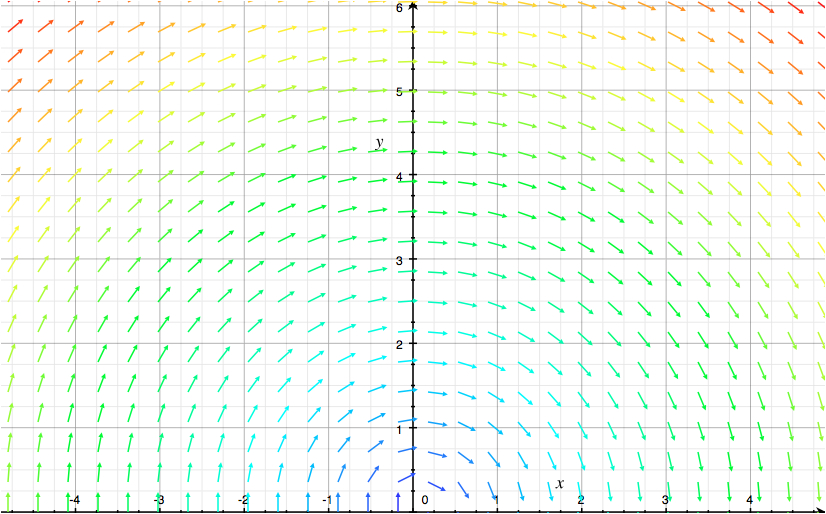
\includegraphics[width=\textwidth]{Bild1} \\
	Rate: $y = \sqrt{r^2 - x^2}$ für $r > 0$
	\[ \implies y' = \frac{-2x}{2 \sqrt{r^2 - x^2}} = \frac{-x}{y} \]
	$(x,y) \mapsto \frac{-x}{y}$ ist lokal Lipsschitz stetig $\implies$ Existenz- und Eindeutigkeitssatz anwendbar. \\
	Zu $(x_0 , y_0) \in U$ gibt $r \coloneqq \sqrt{x_0^2 + y_0^2}$ eine Lösung $x \mapsto \sqrt{r^2 - x^2}$ durch $(x_0 , y_0)$ \\
	$\implies$ das ist \textbf{die} Lösung durch $(x_0 , y_0)$. \\
	max. Existenzintervall $]-r , r [$
\end{bsp}
\begin{bsp}
	$y' = \underbrace{y^2}_{\text{lokal Lipschitz stetig}}$ auf $U = \R^2$ \\
	Rechentrik: Vertausche $x , y$:
	\begin{gather*}
		\begin{split}
			\frac{\dd y}{\dd x} = y^2	&\overset{y \neq 0}{\iff} \frac{\dd x}{\dd y} = \frac{1}{y^2} \iff x = \int \frac{dy}{y^2} = \frac{-1}{y} + c \\
							&\iff \frac{-1}{y} = c - x \iff y = \frac{1}{c - x}
		\end{split} \\
		\intertext{Test:}
		\left( \frac{1}{c - x} \right)' = \frac{\dd}{\dd x} \left( \frac{1}{c - x} \right) = \frac{+1}{(c-x)^2} = \left( \frac{1}{c - x} \right)^2
	\end{gather*}
	$\implies$ Die Funktion $x \mapsto y \coloneqq \frac{1}{c - x}$ ist eine Lösung. $\R \setminus \{c\} \rightarrow \R$ für jedes $c \in \R$. \\
	Diese gilt durch $(x_0 , y_0) \iff x_0 \neq c \wedge y_0 = \frac{1}{c - x} \neq 0 \iff \frac{1}{y_0} = c - x_0 \iff y_0 \neq 0 \wedge c = \frac{1}{y_0} + x_0$ \\
	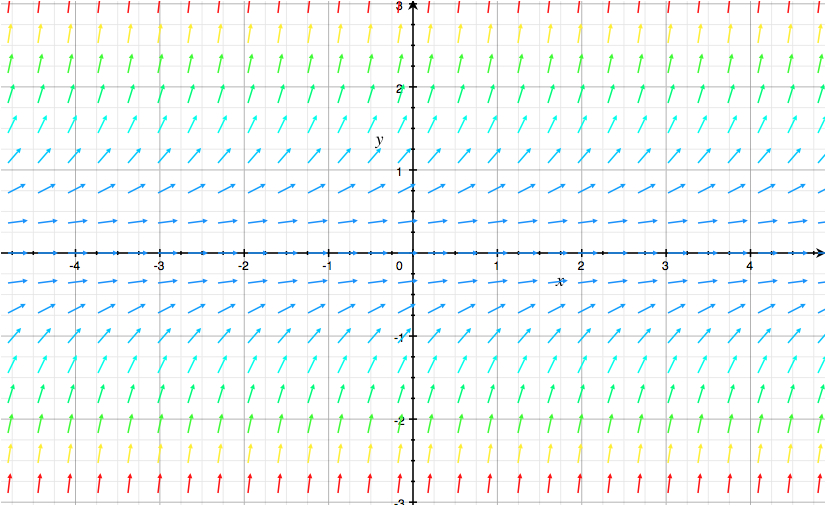
\includegraphics[width=\textwidth]{Bild2}
	$\rightsquigarrow$ Maximallösungen: auf $]-\infty , c[$ oder $] c , \infty [$ sowie $y \equiv 0$ auf $\R$
\end{bsp}
\begin{bsp}
	\[ y' = 3 \abs{y}^{\frac{2}{3}} \]
	Graph ( $y \mapsto 3 \abs{y}^{\frac{2}{3}}$ ) \\
	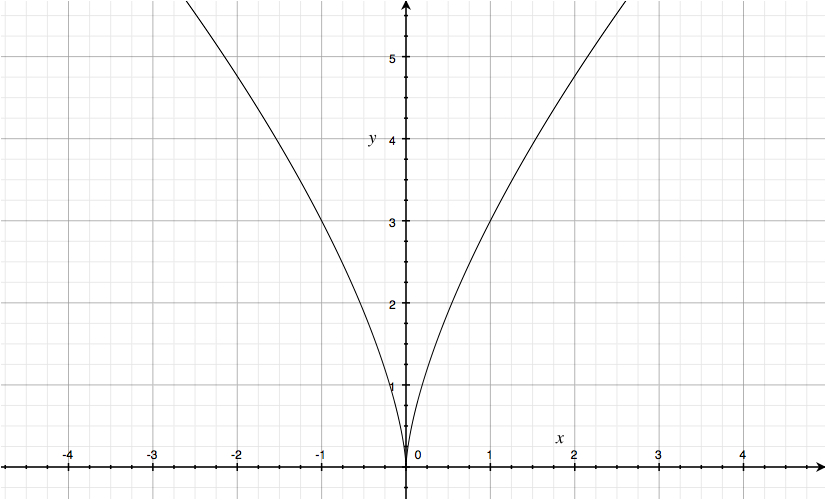
\includegraphics[width=\textwidth]{Bild3} \\
	nicht lokal Lipschitz stetig bei $y=0$
	\begin{gather*}
		\text{Fall } y>0 : \\
		\frac{\dd y}{\dd x} = 3 y^{\frac{2}{3}} \\
		\frac{\dd x}{\dd y} = \frac{1}{3} y^{-\frac{2}{3}} \\
		x = \int \frac{1}{3} y^{-\frac{2}{3}} dy = y^{\frac{1}{3}} + c \\
		y^{\frac{1}{3}} = x - c \\
		y = (x-c)^3
	\end{gather*}
	Diese $> 0 \iff x > c$ \\
	$\rightsquigarrow$ Lösung: $]c , \infty[ \rightarrow \R , x \mapsto (x-c)^3$ \\
	Test: $y' = 3(x-c)^2 = 3 \abs{x-c}^{\frac{2}{3}}$ \\
	Fall $y<0$ \dots \\
	Lösung: $] -\infty , c [ \rightarrow \R , x \mapsto (x-c)^3$
	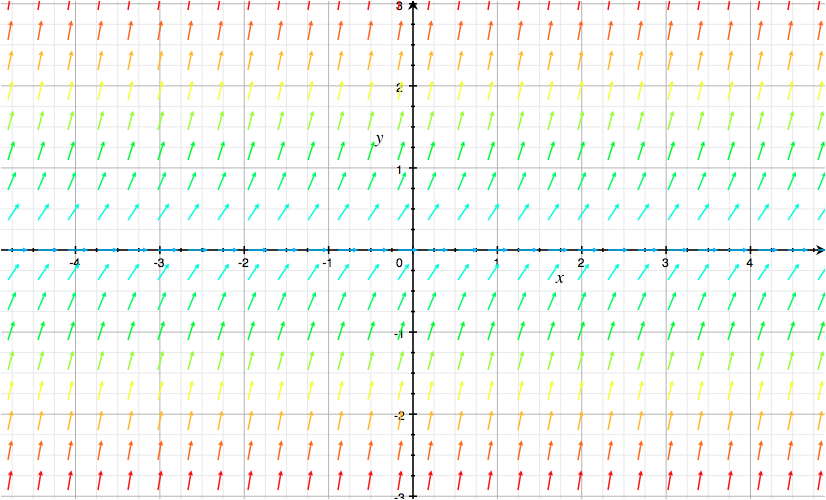
\includegraphics[width=\textwidth]{Bild4} \\
	Leicht: Durch jeden Punkt $(x_0 , y_0)$ mit $y_0 \neq 0$ geht genau eine dieser Lösungen. \\
	Darin ist $\R \rightarrow \R , x \mapsto 0$ eine Lösung. \\
	Jede Lösung auf einem Intervall hat die Gestalt für $-\infty \leq c_2 \leq c_1 \leq \infty$
	\[ y(x) = \begin{cases}
		(x-c_1)^3	&x > c_1			\\
		0		&c_2 \leq x \leq c_1	\\
		(x-c_2)^3	&x < c_2			
	\end{cases} \]
\end{bsp}
\begin{bsp*}
	Finde alle Kurven in $\R^2$, welche die Hyperbeln $xy = \text{const}$ überall sekrecht schneiden (\textbf{Orthogonaltrajektorien}) \\
	Durch $(x_0,y_0)$ geht die Hyperbel $xy = x_0 y_0$
	\begin{gather*}
		xy = x_0 y_0 \\
		y = \frac{x_0 y_0}{x} \\
		\frac{\dd y}{\dd x} = \frac{-x_0 y_0}{x^2} \\
		\left. \frac{\dd y}{\dd x} \right|_{x=x_0} = -\frac{y_0}{x_0} \\
		\text{Orthogonale Steigung: } +\frac{x_0}{y_0}
		\intertext{Gesuchte Kurve hat die Differentialgleichung}
		\frac{\dd y}{\dd x} = \frac{x}{y}
		\intertext{Die ist \textbf{separierbar}. Trick: Multipliziere mit $y \cdot \dd x$} 
		y \dd y = x \dd x \\
		y^2 = \int 2y \dd y = \int 2x \dd x = x^2 + c \\
		y = \pm \sqrt{x^2 + c} \\
		y^2 - x^2 = c \\
		(y-x)(y+x) = c \text{ Drehung um $45^\circ$ Grad}
	\end{gather*}
	Antowort: Alle um $45^\circ$ gedrehten Hyperbeln \\
	Nachrechnen $\rightsquigarrow$ okay, auch für $x=0$ und $y=0$
\end{bsp*}

\section{Lösungen von Differentialgleichungen in Termen bekannter Funktionen und Integralen}
\subsection{Separierbare Differentialgleichungen erster Ordnung}
\[ y' = g(x) \cdot K(y) \]
Ansatz:
\begin{enumerate}[label=(\alph*)]
	\item Für $y_0$ mit $K(y_0) = 0$ ist $y \equiv y_0$ eine Lösung
	\item Für $K(y) \neq 0$ multipliziere mit $\dd x \cdot K(y)^{-1}$
		\begin{gather*}
			\int \frac{\dd y}{K(y)} = \int g(x) \dd x \\
			H(y) = F(x) + c
		\end{gather*}
		$H(y)$ ist lokal invertierbar, da $\frac{dH}{dy}(y) = \frac{1}{K(x)} \neq 0$ \\
		$\rightsquigarrow$ Lösung ist: $y = H^{-1}(F(x) + c)$
\end{enumerate}

\begin{bsp*}
	\begin{gather*}
		\frac{\dd y}{\dd x} = 1 + y^2 \\
		1 + y^2 \neq 0 \text{ immer} \\
		\int \frac{\dd y}{1+y^2} = \int \dd x \\
		\arctan y = x + c \\
		y = \tan(x+c)
	\end{gather*}
\end{bsp*}
\begin{bsp*}
	\begin{gather*}
		\frac{\dd y}{\dd x} = \sqrt{\frac{1-y^2}{1-x^2}} \\
		\text{konstante Lösungen: } y = \pm 1 \\
		\text{nichtkonstante Lösungen:} \\
		\int \frac{\dd y}{\sqrt{1-y^2}} = \int \frac{\dd x}{\sqrt{1-x^2}} \\
		\arcsin y = \arcsin x + c \\
		\begin{split}
			y	&= \sin( \arcsin x + c) \\
				&= x \cdot \cos c + \cos \arcsin x \cdot \sin c \\
				&= x \cdot b \pm \sqrt{1-x^2} \cdot a , a^2 + b^2 = 1 \\
				&= xb + \sqrt{1-x^2} \cdot a
		\end{split}
	\end{gather*}
\end{bsp*}

\subsection{Homogene Differentialgleichungen ertster Ordnung}
\begin{gather*}
	\frac{\dd y}{\dd x} = f(x,y) \text{ mit } f(x,y) = f(cx,cy) \text{ für alle } c , x , y \\
	\text{Äquivalent: } \frac{\dd y}{\dd x} = f\left( 1 , \frac{y}{x} \right) \\
	\text{Ansatz: } u = \frac{y}{x} \\
	\rightsquigarrow \frac{\dd u}{\dd x} = \frac{\frac{\dd y}{\dd x}}{x} - \frac{y}{x^2} = \frac{f(1,u)}{x} - \frac{u}{x} \\
	\frac{\dd u}{\dd x} = \frac{f(1,u) - u}{x} \text{ separierbar}
\end{gather*}
\begin{bsp*}
	\begin{gather*}
		\frac{\dd y}{\dd x} = \frac{y+\sqrt{x^2+y^2}}{x} \\
		\frac{y}{x} = u \rightsquigarrow u + \sqrt{1+u^2} \\
		\rightsquigarrow \frac{\dd u}{\dd x} = \frac{\sqrt{1+u^2}}{x} \\
		\rightsquigarrow \text{ keine konstante Lösungen} \\
		\int \frac{\dd u}{\sqrt{1+u^2}} = \int \frac{\dd x}{x} \\
		\arsinh u = \log\abs{x} + c \\
		\begin{multlined}
			u = \sinh( \log\abs{x} + c) = \sinh\log ax = \frac{e^{\log ax} - e^{-\log ax}}{2} = \\
			\frac{ax - \frac{1}{ax}}{2}
		\end{multlined} \\
		\rightsquigarrow y = ux = \frac{ax - \frac{1}{ax}}{2} \cdot x = \frac{a^2 x^2 - 1}{2a}
	\end{gather*}
\end{bsp*}
\begin{bsp*}
	\begin{gather*}
		\frac{\dd y}{\dd x} = \frac{x+qy}{qx-y} = \frac{1+q\frac{y}{x}}{q-\frac{y}{x}} \\
		u = \frac{y}{x} \rightsquigarrow \frac{\dd x}{\dd y} = \frac{1+qu}{q-u} \\
		\frac{\dd u}{\dd x} = \frac{\frac{1+qu}{q-u} - u}{x} = \frac{\frac{1+u^2}{q-u}}{x} \\
		\rightsquigarrow \int \frac{q-u}{1+u^2} du = \int \frac{\dd x}{x} = \log\abs{x} + c \\
		\text{Linke Seite: } q \cdot \arctan u - \underbrace{\int \frac{u \dd u}{1+u^2}}_{\frac{1}{2} \log(1+u^2)} \\
		q \arctan u - \frac{1}{2} \log(1+u^2) = \log\abs{x} + c
		\intertext{nicht nach $u$ auflösbar. Aber:}
		x = r \cos \varphi \\
		y = r \sin \varphi \\
		\rightsquigarrow u = \tan \varphi \\
		q \varphi \underbrace{- \frac{1}{2} \log \frac{1}{\cos^2 \varphi}}_{+\log\abs{\cos\varphi}} = \underbrace{\log\abs{r \cos\varphi}}_{\log r + \log\abs{\cos\varphi}} + c \\
		q \varphi = \log r + c \\
		r = e^{q \varphi - c} \\
		x = e^{q \varphi - c} \cos\varphi \\
		y = e^{q \varphi - c} \sin\varphi
		\intertext{logarithmische Spirale}
	\end{gather*}
\end{bsp*}

\subsection{Allgemeine lineare Differentialgleichung erster Ordnung}
\[ y' = p(x) \cdot y + q(x) \]
\subsubsection{Homogener Fall}
homogen falls $q(x) \equiv 0$
\begin{gather*}
	\frac{\dd y}{\dd x} = p(x) \cdot y \text{ ist separierbar} \\
	\text{konstante Lösungen: } y \equiv 0 \\
	\log\abs{y} = \int \frac{dy}{y} = \int p(x) \dd x \\
	\underbrace{\log\abs{y} - c}_{\log{\frac{y}{a}} , a \neq 0} = \int p(x) \dd x
	\intertext{allgemeine Lösung der homogenen Differentialgleichung}
	y = a \cdot e^{\int p(x) \dd x} \text{ für alle } a \in \R \text{ konstant}
\end{gather*}
\subsubsection{Inhomogener Fall}
Variation der Konstanten, d.h. ersetze die Konstante durch eine Funktion. \\
Wähle eine nichtriviale Lösung $Y \neq 0$ der homogenen Differentialgleichung: $Y' = p(x) \cdot Y$ \\
\begin{gather*}
	\text{Ansatz: } y(x) = Y(x) \cdot u(x) \\
	\underbrace{y'}_{\substack{=py+q\\=pYu+q}} = (Yu)' = Y'u + Yu' = pYu + Yu' \\
	Yu' = q \\
	u' = \frac{q}{Y} \\
	u(x) = \int \frac{q(x)}{Y(x)} \dd x + c \\
	y(x) = Y(x) \cdot \left[ \int \frac{q(x)}{Y(x)} \dd x + c \right] \\
	y(x) = Y(x) \cdot \int \frac{q(x)}{Y(x)} \dd x + c \cdot Y(x) , c \text{ const.}
\end{gather*}

\begin{bsp}
	\begin{gather*}
		y' = x^3 - xy \\
		\text{homogene DGL: } Y' = -xY \\
		\int -x \dd x = -\frac{x^2}{2} + c \\
		\text{Wähle } Y = e^{-\frac{x^2}{2}} \\
		\implies y(x) = e^{-\frac{x^2}{2}} \cdot \int \frac{x^3}{e^{-\frac{x^2}{2}}} \dd x + c \cdot e^{-\frac{x^2}{2}} \\
		\begin{split}
			\int x^3 e^{\frac{x^2}{2}}	&= \begin{vmatrix} u = \frac{x^2}{2} \\ \dd u = x \dd x \\ x^3 = x^2 x = 2ux \end{vmatrix} \\
								&= \int \underbrace{2u}_{\downarrow} \cdot \underbrace{e^u}_{\uparrow} \dd u \\
								&= 2ue^u - \int 2 e^u \dd u \\
								&= 2ue^u - 2e^u + c \\
								&= 2e^u(u-1) + c \\
								&= 2e^{\frac{x^2}{2}} (\frac{x^2}{x} - 1) + c \\
								&= e^{\frac{x^2}{2}} (x^2 - 2) + c
		\end{split} \\
		y(x) = x^2 - 2 + c e^{-\frac{x^2}{2}} \\
		\text{Probe: } y' = 2x - cxe^{-\frac{x^2}{2}} \\
		x^3 - xy = x^2 - x(x^2 - 2 + ce^{-\frac{x^2}{2}}
	\end{gather*}
\end{bsp}
\begin{bsp}
	\begin{gather*}
		y' + \frac{y}{x} = \sqrt{x} \text{ für } x > 0 \\
		\text{homogene DGL: } Y' + \frac{Y}{x} = 0 \\
		\begin{aligned}
			\text{d.h. } \frac{\dd Y}{\dd x}	&= -\frac{Y}{x} 	&\iff \int \frac{\dd Y}{Y} = -\int \frac{\dd x}{x} \\
									&			&\iff \log\abs{Y} = -\log\abs{x} + c \\
									&= \log\frac{1}{\abs{x}} + c 
		\end{aligned} \\
		Y = \text{ const. } \cdot \frac{1}{x} \\
		\text{Wähle } Y = \frac{1}{x} \rightsquigarrow \frac{q(x)}{Y(x)} = \frac{\sqrt{x}}{\frac{1}{x}} \\
		\text{Ansatz: } y = u \frac{1}{x} \\
		y(x) = \frac{1}{x} \int x^{\frac{3}{2}} \dd x + \frac{c}{x} = \frac{1}{x} \left( \frac{2}{3} x^{\frac{5}{2}} \right) + \frac{c}{x} \\
		\implies y(x) = \frac{2}{3} x^{\frac{3}{2}} + \frac{c}{x}
	\end{gather*}
\end{bsp}

\subsection{Lineare Differentialgleichung zweiter Ordnung}
\[ y'' + p(x) \cdot y' + q(x) \cdot y = r(x) \]
homogen falls $r(x) = 0$
\begin{enumerate}[label=(\alph*)]
	\item Suche Lösungen der homogenen Differentialgleichung $Y'' + pY' + qY = 0$
	\item Variation der Konstanten für inhomogene Gleichung
\end{enumerate}

\begin{bsp*}[note = Ad (b)]
	\begin{gather*}
		y'' + y = \tan x \\
		Y'' + Y = 0
		\text{Errate Lösungen: } \sin x , \cos x \\
		\rightsquigarrow \text{allg. Lösung der homogenen DGL:} \\
		a\cdot \sin x + b \cdot \cos x ; a , b \text{ konstant} \\
		\text{Ansatz: } y =u \sin x + v \cos x \\
		\text{für zu bestimmende Funktionen } u , v \\
		\rightsquigarrow y' = ( u \cos x - v \sin x ) + ( \underbrace{u' \sin x + v' \cos x}_{\text{Setze } = 0} ) \\
		\rightsquigarrow y'' = ( -u \sin x - v \cos x ) + ( u' \cos c - v' \sin x ) \\
		\underbrace{y + y''}_{=\tan x} = u' \cos x - v' \sin x \\
		\\
		u' \sin x + v' \cos x = 0 \\
		u' \cos x - v' \sin x = \tan x
		\intertext{Dies ist ein LGS für $u'$ und $v'$}
		u' ( \underbrace{\sin^2 x + \cos^2 x}_{=1} ) + v' ( \underbrace{\cos x \sin x - \sin x \cos x}_{=0} ) = \underbrace{\tan x \cos x}_{=\sin x} \\
		\rightsquigarrow u' = \sin x \\
		\text{analog: } v' = \frac{-\sin^2 x}{\cos x} \\
		\begin{split}
			\rightsquigarrow	&u = \int \sin x \dd x = -\cos x + \text{ const.} \\
						&v = -\int \frac{sin^2}{\cos x} \dd x = \frac{1}{2} \log\abs{ \frac{1-\sin x}{1+\sin x}} + \sin x + \text{ const.}
		\end{split} \\
		\rightsquigarrow \text{allg. Lösung:} \\
		\begin{split}
			y(x)	&= - \cos x \sin x +  \left( \frac{1}{2} \log\abs{ \frac{1-\sin x}{1+\sin x}} + \sin x \right) \cdot \cos x \\
				&+ a \sin x + b \cos x \\
				&= \frac{1}{2} \cos x \log\abs{ \frac{1-\sin x}{1+\sin x}} + a \sin x + b \cos x \\
				&\text{ für Konstanten  } a , b
		\end{split}
	\end{gather*}
\end{bsp*}
\todo{Too long}
\begin{bsp*}[note = für Lösung mit Potenzreihenansatz]
	Besselsche DGL:
	\begin{gather*}
		f''(x) + \frac{1}{x} f'(x) + \left( 1 - \frac{n^2}{x^2} \right) \cdot f(x) = 0 , n \in \Z^{\geq 0}
		\intertext{Gesucht: alle Lösungen der Form}
		f(x) = \sum_{k=0}^\infty a_k \cdot x^k \text{ für Konstanten } a_k \\
		\begin{split}
			\rightsquigarrow	&f'(x) = \sum_{k=0}^\infty a_k \cdot k \cdot x^{k-1} \\
						&f''(x) = \sum_{k=0}^\infty a_k \cdot k \cdot (k-1) \cdot x^{k-2}
		\end{split} \\
		\begin{split}
			\rightsquigarrow	 0	&= \sum_{k=0}^\infty a_k k (k-1) x^{k-2} \\
							&+ \frac{1}{x} \sum_{k=0}^\infty a_k \cdot k \cdot x^{k-1} \\
							&+ \left( 1 - \frac{n^2}{x^2} \right) \sum_{k=0}^\infty a_k \cdot x^k
		\end{split} \\
		\text{Setze } a_{-1} = a_{-2} = 0 \\
		\begin{split}
			0	&= \sum_{k=0}^\infty x^{k-2} \left[ a_k k (k-1) + a_k k - a_k n^2 \right] + \sum_{k=0}^\infty a_{k-2} x^{k-2} \\
				&= \sum_{k=0}^\infty x^{k-2} \left[ \underbrace{a_k k (k-1) + a_k k - a_k n^2 + a_{k-2}}_{=0 \text{ nach Potenzreihenidentitätssatz}} \right]
		\end{split} \\
		\text{d.h. } \forall k \geq 0 : a_k ( k^2 - n^2 + a_{k-2} = 0 \\
		\rightsquigarrow \forall k \geq 0 : \begin{cases}
			a_k = \frac{a_{k-2}}{n^2 - k_2}	&k \neq n \\
			a_{n-2} = 0				&k = n
		\end{cases} \\
		\begin{split}
			\rightsquigarrow	&a_k = 0 \text{ falls } k \not\equiv n \pmod 2 \\
						&a_k = 0 \text{ falls } k < n
		\end{split} \\
		\text{Setze } a_n = a \\
		\begin{split}
			\rightsquigarrow \text{ für } l \geq 0 \text{ gilt } a_{n+2l}
				&= \frac{a_{n + 2(l-1)}}{-2l(2n+2l)} \\
				&= \frac{-a_{n + 2(l-1)}}{4l(n+l)} \text{ falls } l \geq 1
		\end{split} \\
		\begin{split}
			\implies a_{n+2l}
				&= \frac{(-1)^l \cdot a}{4^l l! (n+l)(n+l-1) \dotsm (n+1)} \\
				&= \frac{(-1)^l \cdot a \cdot n!}{4^l \cdot l! \cdot (n+1)!}
		\end{split}
		\intertext{Antwort: }
		f(x) = \underbrace{c}_{\text{ const.}} \cdot \sum_{l=0}^\infty \frac{(-1)^l \cdot x^{n+2l}}{4^l \cdot l! \cdot (n+1)!}
		\intertext{Die hat Konvergenzradius $\infty$}
	\end{gather*}
\end{bsp*}

\subsection{Lineare Differentialgleichung beliebiger Ordnung}
Funktionen von $x$
\[ y^{(n)} + f_{n-1} \cdot y^{(n-1)} + \dots + f_0 y^{(0)} = g \]
\subsubsection{Homogener Fall}
homogen falls $g=0$, sonst inhomogen \\
Abkürzung: $D \coloneqq \frac{\dd}{\dd x}$. Dann $y' = Dy$
\begin{gather*}
	y'' = DDy = D^2 y \\
	D^n y = y^{(n)} \\
	L \coloneqq D^n + f_{n-1} D^{n-1} + \dots + f_0 D^0 \text{ Differentialoperator $n$-ter Ordnung} \\
	Ly = g
	\intertext{Das ist eine linearer Operator}
	L( y_1 + y_2 ) = Ly_1 Ly_2 \\
	L( \lambda y ) = \lambda L(y) \text{ für $\lambda$ konstant}
	\intertext{D.h. $L$ ist eine lineare Abbildung m Sinne der linearen Algebra}
	\text{z.B. wenn } f_0 , \dotsc , f_{n-1} \in \C^\infty(I) , I \text{ Intervall} \\
	\rightsquigarrow L : C^\infty(I) \rightarrow C^\infty(I)
\end{gather*}
Die Lösungen von $Ly=0$ sind genau der Kern von $L$, also ein Untervektorraum und zwar der Dimension $n$. Denn: die Abbildung
\[ \Kern(L) \rightarrow \R , y \mapsto ( y(x_0) , \dotsc , y(^{(n-1)}(x_0) \]
ist bijektiv nach dem Existenz- und Eindeutigkeitssatz \\
Folgen: 
\begin{enumerate}[label=(\alph*)]
	\item Sind $y_1 , \dotsc , y_n$ linear unabhängige Lösungen, so ist jede Lösung gleich $\lambda_1 y_1 + \dots + \lambda_n y_n$ für Konstanten $\lambda_1 , \dotsc , \lambda_n$
	\item Ist $y_p$ eine \enquote{partikuläre} Lösung von $Ly_p = g$, so hat die allgemeine Lösung $Ly=g$ die Gestalt $y_p + \lambda_1 y_1 + \dots + \lambda_n y_n$ , $\lambda_i$ Konstanten.
\end{enumerate}
d.h. $y_1 , \dotsc , y_n$ sind Basis des Lösungsraumes \\
Ab jetzt: $f_0 , \dotsc , f_{n-1}$ konstant.
d.h. $Ly = y^{(n)} + a_{n-1} y^{(n-1)} + \dots + a_0 y$ mit Konstanten $a_i$
\begin{gather*}
	n=1: \\
	y' + a_0 y = 0 \\
	\frac{\dd y}{\dd x} = - a_0 y \\
	\int \frac{\dd y}{y} \int - a_0 \dd x \\
	\log\abs{y} = - a_0 x + c \\
	y = c' \cdot e^{-a_0 x} \\
	\rightsquigarrow \text{Fundamentallösung } y_1 = e^{-a_0 x} \\
	\\
	\text{Ansatz: } y = e^{\lambda x} , \lambda \text{ konstant} \\
	D e^{\lambda x} = \frac{\dd}{\dd x} (e^{\lambda x}) = \lambda \cdot e^{\lambda x} \\
	D^k e^{\lambda x} = \lambda^k \cdot e^{\lambda x} \\
	\rightsquigarrow L e^{\lambda x} = ( \underbrace{\lambda^n + a_{n-1} \lambda^{n-1} + \dots + a_1 \lambda + a_0}_{\text{charakteristisches Polynom von } L \eqqcolon \ch_L(\lambda)} ) e^{\lambda x} \\
	\rightsquigarrow e^{\lambda x} \text{ ist Lösung von } Ly = 0 \text{ \gdw } \lambda \text{eine Nullstelle von $\ch_L(\lambda)$ ist.}
\end{gather*}
\begin{fakt}
	Falls $\ch_L(\lambda)$ nur einfache Nullstellen $\lambda_1 , \dotsc , \lambda_n$ hat, sind $e^{\lambda_1 x} , \dotsc , e^{\lambda_n x}$ Fundamentallösungen von $Ly=0$
\end{fakt}
\begin{bsp*}
	\begin{gather*}
		Ly = y'' + 6y' + 8y = 0 \\
		\rightsquigarrow \ch_L(\lambda) = \lambda^2 + 6\lambda + 8 = (\lambda + 4)(\lambda + 2) = 0 \\
		\iff \lambda = -2 , -4 \\
		\text{allgemeine Lösung: } a \cdot e^{-2x} + b \cdot e^{-4x} \text{ für Konstanten } a , b
	\end{gather*}
\end{bsp*}
\begin{bsp*}
	\begin{gather*}
		y'' + 9y = 0 \\
		\ch_L(\lambda) = \lambda^2 + 9 = 0 \\
		\iff \lambda = \pm 3\imath \\
		\text{allgemeine Lösung: } a \cdot e^{3\imath x} + b \cdot e^{-3\imath x} ; a , b \in \C \text{ konstant} \\
		\text{ allgemeine reelle Lösungen: } \\
		a ( \cos 3x + \imath \sin 3x ) + b( \cos x - \sin 3x ) \\
		= \underbrace{(a+b)}_{c} \cos 3x + \underbrace{(a-b)}_{d} \imath \sin 3x \\
		\text{allgemeine Lösung: } c \cdot \cos 3x + d \cdot \sin 3x \\
		\text{komplexe Lösung: } c , d \in \C \\
		\text{reelle Lösung: } c , d \in \R
	\end{gather*}
\end{bsp*}
\begin{bsp*}
	\begin{gather*}
		y'' - 2y' + 2y = 0 \\
		\ch_L(\lambda) = \lambda^2 - 2\lambda + 2 = 0 = (\lambda - 1 - \imath)(\lambda - 1 + \imath) = 0 \\
		\iff \lambda = 1 \pm \imath \\
		\rightsquigarrow \text{ Fundamentallösungen: } \\
		e^{(1\pm\imath)x} = e^x \cdot e^{\pm\imath x} = e^x ( \cos x \pm \imath \sin x ) \\
		\text{Äquivalente Fundamentallösungen: } e^x \cos x , e^x \sin x
	\end{gather*}
\end{bsp*}
\begin{bsp*}
	\begin{gather*}
		y^{(4)} + 2y'' - 8y' + 5y = 0 \\
		\begin{split}
			\ch_L(\lambda)	&= \lambda^4 + 2\lambda^2 - 8\lambda + 5 \\
						&= (\underbrace{\lambda - 1}_{\text{doppelte Nullstelle } 1})^2 (\underbrace{\lambda^2 + 2\lambda + 5}_{\text{Nullstelle } -1 \pm 2\imath}) \\
						&= 0
		\end{split} \\
		\rightsquigarrow 3 \text{ linear unabhängige Lösungen: } e^x , e^{(-1 \pm 2\imath) x} \\
		\\
		\text{Vergleiche: } y'' = 0 \text{ hat } \ch_L(\lambda) = \lambda^2 \\
		\text{Fundamentallösungen: } \underbrace{1}_{e^{0x}} , \underbrace{x}_{\text{zusätzliche Lösung}} \\
		\intertext{Aber $xe^x$ ist eine weitere Lösung, und die allgemeine Lösung lautet}
		ae^x + bxe^x + ce^{(-1+2\imath)x} + de^{(-1+2\imath)x}
	\end{gather*}
\end{bsp*}
Allgemein: Jede Nullstelle $\lambda$ con $\ch_L$ der Multiplizität $k \geq 1$ liefert Fundamentallösungen $e^{\lambda x} , xe^{\lambda x} , \dotsc , x^{k-1} e^{\lambda x}$. \\
Wieso: Schreibe $y =  z \cdot e^{\lambda x} , z = z(x)$ \\
\begin{gather*}
	Ly = L(z \cdot e^{\lambda x}) \\
	D( z \cdot e^{\lambda x} ) = \frac{\dd z}{\dd x} \cdot e^{\lambda x} + \lambda  z \cdot e^{\lambda x} = \left( \frac{\dd z}{\dd x} + \lambda z \right) \cdot e^{\lambda x} = ((D+\lambda)(z)) \cdot e^{\lambda x} \\
	\implies D^k ( z \cdot e^{\lambda x} ) = ((D+\lambda)^k (z)) \cdot e^{\lambda x} \\
	\implies \text{ Ist } L = D^n + a_{n-1} D^{n-1} + \dots + a_0 \text{ so gilt } L(  z \cdot e^{\lambda x} ) = 0 \\
	\iff ( \underbrace{(D+\lambda)^n + a_{n-1} (D+\lambda)^{n-1} + \dots + a_0}_{L'} ) z = 0 \\
	\ch_{L'} = \ch_L(\lambda' + \lambda)
\end{gather*}
Also ist $\lambda$ $k$-fache Nullstelle con $\ch_L$ $\iff \lambda' = 0$ $k$-fache Nullstelle con $\ch_L$ $\iff$ $L' = D^n + \dots + *D^k$ $\implies z = 1 , x , \dotsc , x^{k-1}$ sind Lösungen!

\begin{bsp*}
	\begin{gather*}
		y^{(4)} + 2y'' + y = 0 \\
		\ch_L(\lambda) = \lambda^4 + 2\lambda^2 + 1 = (\lambda^2 + 1)^2 = (\lambda - \imath)^2 (\lambda + \imath)^2 = 0 \\
		\text{doppelte Nullstelle } \pm \imath \\
		\rightsquigarrow \text{ allgemeine Lösungen: lineare Kombinationen von } \\
		e^{\imath x} , x e^{\imath x} , e^{-\imath x} , x e^{-\imath x} \\
		\text{ allgemeine reelle Lösungen: lineare Kombinationen von } \\
		\cos x , \sin x , x \cos x , x \sin x
	\end{gather*}
\end{bsp*}
\begin{bsp*}[note = gedämpfter harmonischer Oszillator]
	\begin{gather*}
		Ly = m \cdot \ddot{y} + b \cdot \dot{y} + f \cdot y \\
		m , f > 0 , b \geq 0 \\
		\text{Eigenwerte: } \lambda = \frac{-b \pm \sqrt{b^2 - 4 fm}}{2m} \\
		b = 0 : \lambda = \pm \frac{\sqrt{4fm}}{2m} \cdot \imath = \nu i \\
		\rightsquigarrow \text{ Fundamentallösungen: } \cos \nu t , \sin \nu t \\
		0 < b < \sqrt{4fm} : \text{ kleine Reibung: } \\
		\lambda = - \mu \pm \imath \nu , \nu \neq 0 , \mu > 0 \implies e^{-\mu t}\cdot \cos \nu t , e^{-\mu t} \sin \nu t \\
		b = \sqrt{4fm} : \lambda = \frac{-b}{2m} \text{ doppelte Nullstelle } e^{\lambda b} , b \cdot e^{\lambda b} \\
		b > \sqrt{4fm} : e^{\lambda_1 b} , e^{\lambda_2 b} für 0 > \lambda_1 > \lambda_2
	\end{gather*}
\end{bsp*}
\begin{bsp*}[note = Randwertproblem]
	Hat die DGL $y'' = y$ eine Lösung mit $y(0) = y(1) = 1$?
	charakteristische Gleichung: $\lambda^2 - 1 = 0$ \\
	Eigenwerte $\pm 1$ \\
	allgemeine Lösung $ae^x + be^{-x}$ \\
	Einsetzen:
	\begin{gather*}
		a + b = 1 \\
		ae + be^-1 = 1
		\intertext{Antwort:}
		y = \frac{e^x + e^{1-x}}{e+1}
	\end{gather*}
\end{bsp*}
\begin{bem}
	Asymptotisches Verhalten für $x \rightarrow \infty$ oder $x \rightarrow -\infty$ ($\overset{\wedge}{=}$ Randbedingung bei $\pm \infty$) \\
	$x^j e^{\lambda x} \rightarrow $ \gdw $\Re(\lambda) < 0$ ist, denn $\abs{e^{\lambda x}} = e^{\Re(x) \cdot x}$ \\
	$x^j e^{\lambda x}$ für $x \rightarrow 0$ beschränkt $\iff \Re(\lambda) < 0 \vee ( \Re(\lambda) = 0 \wedge j = 0 )$ \\
	Entsprechend: eine Linearkombination solchen Funktionen geht gegen $0$ (bzw. bleibt beschränkt) \gdw jeder Summand es tut.
\end{bem}

\subsubsection{Inhomogener Fall}
\begin{fakt}
	Ist $g(x) = a \cdot e^{\lambda x} ; a , \lambda$ konstant und $\lambda$ kein Eigenwert von $L$, dann existiert eine partikuläre Lösung von $Ly = g$ mit $y = b \cdot e^{\lambda x} ; b$ konstant. \\
	Denn:
	\begin{gather*}
		L(b e^{\lambda x} = b L(e^{\lambda x}) = b \underbrace{\ch_L(\lambda)}_{\neq 0} e^{\lambda x} \\
		\intertext{und}
		b \coloneqq \frac{a}{\ch_L(\lambda)} \text{ tut's!}
	\end{gather*}
\end{fakt}
\begin{fakt}
	Entsprechend Linearkombintationen: Sind $Ly_k = g_k(x)$ für $k=1 , \dotsc , m$, dann ist $L(y_1 + \dots + y_m) = g_1(x) + \dots + g_m(x)$
\end{fakt}
\begin{bsp*}
	Bestimme alle Lösungen der DGL
	\[ y^{(4)} + 2y'' - 8y' + 5y = e^{-x} \]
	die für $x \rightarrow \infty$ beschränkt bleiben. \\
	Lösung:
	\begin{gather*}
		\begin{split}
			\ch_L(\lambda)	&= \lambda^4 + 2\lambda^2 - 8\lambda + 5 = 0 \\
						&= (\lambda - 1)(\lambda^3 + \lambda^2 + 3\lambda - 5) \\
						&= (\lambda - 1)^2(\lambda^2+ 2\lambda + 5)
		\end{split} \\
		\lambda = +1 \text{ mit Multiplizität } 2 \\
		\lambda = -1 \pm 2\imath \text{ mit Multiplizität } 1 \\
		\lambda = -1 \text{ ist kein EW!}
		\intertext{Ansatz: partikuläre Lösung}
		y= be^{-x} ; Ly = e^{-x} \\
		\text{Ausrechnen } \rightsquigarrow b = \frac{1}{16}
		\intertext{allgemeine Lösung der inhomogener Gleichung}
		 \frac{1}{16} e^{-x} + ( \alpha + \beta x) e^x + \gamma e^{(-1+2\imath)x} + \delta e^{(-1-2\imath)x}
	\end{gather*}
\end{bsp*}
\begin{fakt}
	Ist $\lambda$ eine Nullstelle  von $\ch_L$ der Multiplizität $m \geq 1$, dann hat $Ly = a e^{\lambda x}$ eine partikuläre Lösung der Gestalt $y = bx^me^{\lambda x} , b$ konstant.
\end{fakt}
\begin{fakt}
	Ist $\lambda$ eine Nullstelle der Ordnung $m$ von $\ch_L$, und $P(x)$ ein Polynom von Grad $l$, so hat $Ly = P(x) e^{\lambda x}$ eine partikuläre Lösung der Form $y = Q(x) e^{\lambda x}$
\end{fakt}
\begin{bsp*}
	 \begin{gather*}
	 	y^{(5)} + y = xe^x \\
	 	\ch_L(\lambda) = \lambda^5 + 1 \\
	 	\lambda = 1 \text{ ist keine Nullstelle}
	 	\intertext{Ansatz für partikuläre Lösung:}
	 	y = (a+bx) e^x =ae^x + bxe^x \\
	 	y^{(5)} = ae^x + bxe^x + 5be^x \\
	 	\rightsquigarrow \underbrace{y^{(5)} + y}_{=xe^x} = (\underbrace{a+a+ 5b}_{0})e^x + (\underbrace{b + b}_{1})xe^x \\
	 	\rightsquigarrow b = \frac{1}{2} ; 2a + 5b = 0 \implies a = -\frac{5}{2} b = -\frac{5}{4} \\
	 	\intertext{$\rightsquigarrow$ partikuläre Lösung:}
	 	y = \left( -\frac{5}{4} + \frac{1}{2}x \right) e^x
	\end{gather*}
\end{bsp*}
\begin{fakt}[note = Variante: falls alle Koeffizienten reell:]
	Ist $\lambda = \mu + \imath\nu ; \mu , \nu \in \R  ; \nu \neq 0$, Nullstelle der Ordnung $m$, so hat $Ly = P_1(x) \cdot e^{\mu x} \cdot \cos \nu x + P_2(x) \cdot e^{\mu x} \cdot \sin \nu x$ mit reelen Polynomen $P_1 , P_2$ eine partikuläre Lösung der Gestalt $y = Q_1(x) \cdot e^{\mu x} \cdot \cos \nu x + Q_2(x) \cdot e^{\mu x} \cdot \sin \nu x$ mit reellen Polynomen $Q_1 , Q_2$ von Grad $\leq m+l$
\end{fakt}
\begin{bsp*}[note = Angeregter harmonischer Oszillator]
	\begin{gather*}
		\ddot{y} + \omega^2 y = \cos \lambda t ; \omega , \lambda \in \R \\
		\ch_L(T) = T^2 + \omega^2 \text{ hat Nullstellen } \pm \imath\omega \\
		\text{Fall 1: } \lambda \pm\imath \omega \leftrightarrow \i\lambda \text{ keine Nullstelle con } \ch_L(T) \\
		\rightsquigarrow \text{ Ansatz: }  y_p(t) = a \cos \lambda t + b \sin \lambda t \qquad \omega^2 \\
		\text{Einsetzen: } \ddot{y_p} = -a \lambda^2 \cos \lambda t - b \lambda^2 \sin \lambda t \\
		\begin{split}
			\cos \lambda t
				&= \ddot{y_p} + \omega^2 y_p \\
				&= a( \omega^2 - \lambda^2) \cos \lambda t + b(\underbrace{\omega^2 - \lambda^2}_{\neq 0}) \sin \lambda t \\
				&= \dots
		\end{split} \\
		\rightsquigarrow b = 0 , a = \frac{1}{\omega^2 - \lambda^2} \\
		y_p = \frac{\cos \lambda t}{\omega^2 - \lambda^2} \\
		\\
		\text{Fall 2: } \lambda = \pm \omega \\
		\text{Ansatz: } at \cos\lambda t + bt \sin \lambda t \\
		\vdots \\
		\implies y_p(t) = \frac{t \sin \lambda t}{2\lambda} \\
		\\
		\text{allgemeine Lösung: } \\
		y_p + c \cos \omega t + d \sin \omega t
	\end{gather*}
\end{bsp*}

\subsection{Systeme von linearen Differentialgleichungen erster Ordnung mit konstanten Koeffizienten}
\begin{gather*}
	y_1 , \dotsc , y_m \text{ Funktionen von } x \\
	\frac{\dd y_1}{\dd x} = F_1( x , y_1 \dotsc , y_m ) = a_{11} y_1 + \dots + a_{1m} y_m + g_1(x) \\
	\vdots \\
	\frac{\dd y_n}{\dd x} = F_1( x , y_1 \dotsc , y_m ) = a_{n1} y_1 + \dots + a_{nm} y_m + g_n(x)
\end{gather*}
Betrachte ein System von lineare Differentialgleichungen mit konstanten Koeffizienten.
\begin{gather*}
	y' = Ay + g \\
	y = \begin{pmatrix} y_1 \\ \vdots \\ y_n \end{pmatrix} , A = \begin{pmatrix} a_{11} & \dots & a_{1n} \\ \vdots & \ddots & \vdots \\ a_{n1} & \dots & a_{nn} \end{pmatrix} , g = \begin{pmatrix} g_1 \\ \vdots \\ g_n \end{pmatrix} \\
	g=0 : \text{ Ansatz: } y = e^{\lambda x} \cdot v , v \text{ konstanter Vektor} \\
	\underbrace{y'}_{Ay} = \underbrace{\lambda e^{\lambda x} \cdot v}_{e^{\lambda x} \cdot Av} \iff Av = \lambda v \\
	\iff v \text{ ist Eigenvektor von $A$ zum Eigenwert } \lambda \in \C
\end{gather*}
Für $\ch_A(\lambda) = \det(\lambda Id_n - A) = 0$charakteristische Gleichung \\
Falls alle Nullstellen $\lambda_1 , \dotsc , \lambda_n$ Multiplizität $1$ haben, zum Eigenvektor $v_1 , \dotsc , v_n$ $\rightsquigarrow$ $e^{\lambda_1 x} v_1 , \dotsc , e^{\lambda_n x} v_n$ ist Basis des Lösungsraums \\
Genauso wenn $\C^n$ eine Basis aus Eigenvektoren hat. \\
Im allgemeinen existiert eine Basis aus Funktionen der Form
\[ e^{\lambda x} \cdot (\text{ Polynom in $x$ mit Koeffizienten in $\C^n$} ) \]
Für $g(x) =$ Linearkombination von $x^j e^{\lambda x}$ für irgendwelche $j , \lambda$ existiert eine Lösung als Linearkombination von $x^j e^{\lambda x}$ für dieselben $\lambda$ aber beliebige $j$ \\
\begin{bsp*}
	\begin{gather*}
		y'_1 = -y_1 + 3y_2 \\
		y'_2 = 2y_1 - 2y_2 \\
		y_1(0) = 5 \\
		y_2(0) = 0 \\
		y = \begin{pmatrix} y_1 \\ y_2 \end{pmatrix} ; A = \begin{pmatrix} -1 & 3 \\ 2 & -2 \end{pmatrix} \\
		\begin{split}
			\ch_A(\lambda)	&= \begin{vmatrix} \lambda + 1 & -3 \\ -2 & \lambda + 2 \end{vmatrix} \\
						&= (\lambda + 1)(\lambda + 2) - (-2)(-3) \\
						&= \lambda^2 + 3\lambda - 4 \\
						&= (\lambda - 1)(\lambda + 4)
		\end{split} \\
		\text{EV} : 
		\lambda = 1 : \begin{pmatrix} 3 \\ 2 \end{pmatrix} \\
		\lambda = -4 : \begin{pmatrix} -1 \\ 1 \end{pmatrix} \\
		\rightsquigarrow \text{ allgemeine Lösungen } y(x) = ae^x \begin{pmatrix} 3 \\ 2 \end{pmatrix} + be^{-4x} \begin{pmatrix} -1 \\ 1 \end{pmatrix} \\
		y(0) = \begin{pmatrix} 3a - b \\ 2a+ b \end{pmatrix} = \begin{pmatrix} 5 \\ 0 \end{pmatrix}
		a = 1 \\
		b = -2 \\
		\text{Lösung: } y(x) = \begin{pmatrix} 3e^x + 2e^{-4x} \\ 2e^x - 2e^{-4x} \end{pmatrix}
	\end{gather*}
\end{bsp*}
\begin{bsp*}[note = Zwei Körper Problem]
	$n$ Körper der Massen $m_i \quad (1 \leq i \leq n)$ im $\R^3$ im Ort $z_i \in \R^3$. \\
	Newtonscher Gravitationsgesetz: \\
	Zwischen $m_i$ und $m_j$ wirkt die Kraft
	\[ \frac{G m_i m_j}{\abs{z_i - z_j}^2} \]
	$\rightarrow$ Kraftvektor
	\[ \frac{G m_i m_j}{\abs{z_i - z_j}^3} (z_j - z_i) \]
	Totalkraft auf $m_i$
	\[ \sum_{\substack{j = 1 \\ j \neq i}}^n \frac{G m_i m_j}{\abs{z_i - z_j}^3} (z_j - z_i) = m_i \cdot \ddot{z_i} \]
	System von $3n$ gekoppelten nichtlinearen Differentialgleichungen 2\textsuperscript{ter} Ordnung. \\
	Ab jetzt: $n=2$ \\
	12 Parameter \\
	\begin{gather*}
		z_0 \coloneqq \frac{m_1 \cdot z_1 + m_2 \cdot z_2}{m_1 + m_2} \\
		\begin{split}
			\implies \ddot{z_o}
				&= \frac{1}{m_1 + m_2} ( m_1 \ddot{z_1} + m_2 \ddot{z_2} ) \\
				&= \frac{1}{m_1 + m_2} \left( \frac{G m_1 m_2}{\abs{z_2 - z_1}^3} (z_2 - z_1) + \frac{G m_1 m_2}{\abs{z_1 - z_2}^3} (z_1 - z_2) \right) \\
				&= 0
		\end{split} \\
		\implies z_0(t) = z_0(0) + \dot{z_0}(0) \cdot t \\
		\text{Ersetze $z_i$ durch $z_i - z_0$ $\implies$ oBdA $m_1 z_1 + m_2 z_2 = 0$} \\
		\\
		\text{Zur Vereinfachung setze } z \coloneqq m_1 z_1 = -m_2 z_2 \\
		\implies z_2 - z_1 = - \frac{z}{m_2} - \frac{z}{m_1} = -\left( \frac{1}{m_1} + \frac{1}{m_2} \right) z \\
		\begin{split}
			\implies \ddot{z}
				&= m_1 \cdot \ddot{z_1} \\
				&= \frac{G m_1 m_2}{\abs{z_2 - z_1}^3} ( z_2 - z_1 ) \\
				&= \frac{ -G m_1 m_2}{\abs{\frac{1}{m_1} + \frac{1}{m_2}}^3 \cdot \abs{z}^3} \cdot \left( \frac{1}{m_1} + \frac{1}{m_2} \right) \cdot z
		\end{split} \\
		\ddot{z} = -\frac{G m_1^3 m_2^3}{(m_1 + m_2)^2} \cdot \frac{z}{\abs{z}^3} \\
		\text{Ersetze $z$ durch $\lambda z$ für geeignetes $\lambda \in \R^{>0}$ } \rightsquigarrow \ddot{z} = -\frac{z}{\abs{z}^3}
	\end{gather*}
	\begin{beh}
		Die Lösung bleibt in dem von $z(0) \neq 0 , \dot{z}(0)$ aufgespannten Teilraum $U$ \\
		\begin{bew}[head = Denn:]
			Invarianz unter Drehungen $\implies$ oBdA $U = \begin{pmatrix} * \\ 0 \\ 0 \end{pmatrix} , \begin{pmatrix} * \\ * \\ 0 \end{pmatrix}$ \\
			Dann betrachte dieselbe DGl. nur für $z \in U$. Die hat eine Lösung, und diese ist auch eine Lösung in $\R^3$ Lösung in $\R^3 \underset{\text{Eindeutigkeit}}{\implies}$ Dies ist \textbf{die} Lösung in $\R^3$
		\end{bew}
	\end{beh}
	\begin{gather*}
		\dim U = 1 : \text{ eine gewöhnliche DGl. 2\textsuperscript{ter} Ordnung} \\
		\text{ab jetzt $\dim U = 2$} \\
		\text{Ersetze $\R^3$ durch $\R^2 = \C$} \\
		\text{Polarkoordinaten: } z = r e^{\imath\varphi} \\
		\implies \dot{z} = \dot{r} e^{\imath\varphi} + r \imath \dot{\varphi} e^{\imath\varphi} \\
		\ddot{z} = \ddot{r} e^{\imath\varphi} + 2 \dot{r} \imath \dot{\varphi} + r ( \imath \ddot{\varphi} e^{\imath\varphi} + (\imath \dot{\varphi})^2 e^{\imath\varphi} ) \\
		- \frac{z}{\abs{z}^3} = \frac{-r e^{\imath\varphi}}{r^3} = -\frac{1}{r^2} e^{\imath\varphi} \\
		\rightsquigarrow \ddot{r} + 2 \dot{r} \imath \dot{\varphi} + r ( \imath \ddot{\varphi} - \dot{\varphi}^2 ) = -\frac{1}{r^2} \\
		\iff \begin{cases}
			\ddot{r} - r \dot{\varphi}^2 = -\frac{1}{r^2} \\
			2 \dot{r} \dot{\varphi} + r \ddot{\varphi} = 0 
		\end{cases} \\
		\\
		\text{Erhaltungsgrössen:} \\
		\text{Winkelmoment } \mu \coloneqq r^2 \cdot \dot{\varphi} \\
		\dot{\mu} = 2 r \dot{r} \dot{\varphi} + r^2 \ddot{\varphi} = r ( 2 \dot{r} \dot{\varphi} + r \ddot{\varphi} ) = 0 \\
		\implies \mu \text{ konstant} \\
		\text{Energie } E \coloneqq \frac{\abs{\dot{z}}^2}{2} - \frac{1}{\abs{z}} \\
		E = \frac{\abs{\dot{r} + r \imath \dot{\varphi}}^2}{2} - \frac{1}{r} = \frac{ \dot{r}^2  + r^2 \dot{\varphi}^2}{2} - \frac{1}{r} \\
		\dot{E} = \dots = 0 \\
		\implies E \text{ konstant} \\
		\dot{\varphi} = \frac{\mu}{r^2} \implies E = \frac{\dot{r}^2 + \frac{\mu^2}{r^2}}{2} - \frac{1}{r} \\
		\rightsquigarrow \begin{cases}
			\dot{\varphi} = \frac{\mu}{r^2} \\
			\dot{r}^2 = 2 E + \frac{2}{r} - \frac{\mu^2}{r^2}
		\end{cases} \\
		\frac{\dd r}{\dd t} = \pm \sqrt{2E + \frac{2}{r} - \frac{\mu^2}{r^2}} \\
		\int \frac{\pm \dd r}{\sqrt{2E + \frac{2}{r} - \frac{\mu^2}{r^2}}} = \int \dd t \\
		\frac{\dd r}{\dd \varphi} = \frac{\frac{\dd r}{\dd t}}{\frac{\dd \varphi}{\dd t}} = \frac{\pm\sqrt{2E + \frac{2}{r} - \frac{\mu^2}{r^4}}}{\frac{\mu}{r^2}} \\
		\text{Variablentransformation: } u = \frac{1}{r} \\
		\begin{multlined}
			\left( \frac{\dd u}{\dd \varphi} \right)^2 = \left( \frac{-1}{r^2} \frac{\dd r}{\dd \varphi} \right)^2 = \frac{1}{r^4} \cdot \frac{2E + \frac{2}{r} - \frac{\mu^2}{r^2}}{\left( \frac{\mu}{r^2} \right)^2} = \\
			\frac{1}{\mu^2} \cdot \left( 2E + 2u - \mu^2 u^2 \right) 
		\end{multlined} \\
		\left( \frac{\dd u}{\dd \varphi} \right)^2 = \underbrace{\left( \frac{2E}{\mu^2} + \frac{1}{\mu^4} \right)}_{H^2 \geq 0 \text{ für } H \geq 0} - \left( u - \frac{1}{\mu^2} \right)^2 \\
		\text{Substitution: } v = H^{-1} \left( u - \frac{1}{\mu^2} \right) \\
		\rightsquigarrow \left( \frac{\dd u}{\dd \varphi} \right)^2 = \left( H \cdot \frac{\dd v}{\dd \varphi} \right)^2 = H^2 - H^2 v^2 \\
		\left( \frac{\dd v}{\dd \varphi} \right)^2 = 1 - v^2 \\
		v = \sin( \varphi - \varphi_0 ) \\
		r = \frac{\mu^2}{1 + H\mu^2 \sin( \varphi - \varphi_0 ) }  \\
		x = r \cdot \cos \varphi \\
		y = r \cdot \sin \varphi \\
		\text{Nach Drehung oBdA } \varphi_0 = 0 \\
		\text{Einsetzen und Ausrechnen} \\
		\vdots \\
		\rightsquigarrow x^2 = 2E \mu^2 y^2 - 2H \mu^4 y + \mu^4 \\
		E < 0 \implies \text{ Ellipse} \\
		E = 0 \implies \text{ Parabel} \\
		E > 0 \implies \text{ Hyperbel}
	\end{gather*}
\end{bsp*}

\section{Differentialrechnung in mehreren Variablen}
\[ \R^n \supset U \rightarrow V \subset \R^m \]
\begin{bsp*}
	\[ f(x,y) = x^2 \cdot \cos y \]
	Fixiere $x$ und betrachte die Ableitung nach $y$: $\frac{\partial f}{\partial y}$ \\
	Fixiere $y$ und betrachte die Ableitung nach $x$: $\frac{\partial f}{\partial x}$
\end{bsp*}
Sei $U \subset \R^n$ offen , $f: U \rightarrow \R$ \\
\begin{def*}[note = partielle Differenzierbarkeit , index = partiel differenzierbar , indexformat = {2!1~}]
	$f$ heisst partiell differenzierbar in $\begin{pmatrix} x_1 \\ \vdots \\ x_n \end{pmatrix}$ falls für alle $1 \leq i \leq n$ die \textbf{partielle Ableitung}
	\[ \frac{\partial f}{\partial x_i} \coloneqq \lim_{h \rightarrow 0} \frac{f\begin{pmatrix} x_1 \\ \vdots \\ x_i + h \\ \vdots \\ x_n \end{pmatrix} - f\begin{pmatrix} x_1 \\ \vdots \\ x_i \\ \vdots \\ x_n \end{pmatrix}}{h} \]
	existiert.
\end{def*}
\begin{def*}[note = Richtungsableitung , index = Richtungs Ableitung , indexformat = {2!1-~}]
	Sei $e \in \R^n$ ein Einheitsvektor. \\
	Die \textbf{Richtungsableitung} von $f$ in $x \in U$ in Richtung $e$ ist
	\[ \begin{split}
		(D_e f)(x)	&\coloneqq \left.\left( \frac{\dd}{\dd t} f(x + te) \right)\right|_{t=0} \\
				&= \lim_{t \rightarrow 0} \frac{f(x+te) - f(x)}{t}
	\end{split} \]
	Also:
	\[ e_i = \begin{pmatrix} 0 \\ \vdots \\ 1 \leftarrow i \\ \vdots \\ 0 \end{pmatrix} \rightsquigarrow D_{e_i} f = \frac{\partial f}{\partial x_i} \]
\end{def*}
D.h.:
\[ f(x + te) = f(x) + (D_e f)(x) \cdot t + o(t) \]
\begin{gather*}
	x = \begin{pmatrix} x_1 \\ \vdots \\ x_n \end{pmatrix} \in U , e = \begin{pmatrix} e_1 \\ \vdots \\ e_n \end{pmatrix} \text{ Einheitsvektor } ; f: U \rightarrow \R \\
	f \text{ partiell differenzierbar } \\
	\iff \forall i : f\left( \begin{pmatrix} x_1 \\ \vdots \\ x_n \end{pmatrix} + \begin{pmatrix} 0 \\ \vdots \\ 1 \leftarrow i \\ \vdots \\ 0 \end{pmatrix} \cdot h \right) = f(x) + \frac{\partial f}{\partial x_i} + o(h) \\
	f \text{ in Richtung $e$ differenziebar } \\
	\iff f\left( \begin{pmatrix} x_1 \\ \vdots \\ x_n \end{pmatrix} + \begin{pmatrix} e_1 \\ \vdots \\ e_n \end{pmatrix} \cdot t \right) = f(x) + D_e f(x) \cdot t + o(t) \\
	f \text{ (total) differenzierbar } \\
	\begin{multlined}
		\iff f\left( \begin{pmatrix} x_1 \\ \vdots \\ x_n \end{pmatrix} + \begin{pmatrix} h_1 \\ \vdots \\ h_n \end{pmatrix} \right) = f(x) + ( A_1 h_a + \dots + A_n h_n ) + o( \abs{h} ) ; \\
		h =  \begin{pmatrix} h_1 \\ \vdots \\ h_n \end{pmatrix}
	\end{multlined}
\end{gather*}
Dabei heisst $(A_1 , \dotsc , A_n) = \grad f = \nabla f$ (\enquote{nabla}) der \textbf{Gradient} von $f$ in $x$ oder die (totale) Ableitung von $f$ in $x$
Ist $f$ total differenzierbar, dann ist
\[ \begin{split}
	f(x+te)
		&= f(x) + (A_i t e_1 + \dotsb + A_n t e_n ) + o( \abs{te} ) \\
		&= f(x) + (A_1 e_1 + \dotsb + A_n e_n) t + o(t) 
\end{split} \]
Also ist $f$ in jede Richtung $e$ differenzierbar, und $D_e f = (\grad f) \underbrace{\cdot}_{\text{Matrixprodukt}} e$ \\
\begin{bem}
	total differenziebar $\begin{matrix} \Rightarrow \\ \not\Leftarrow \end{matrix}$ in jede Richtung differenzierbar $\begin{matrix} \Rightarrow \\ \not\Leftarrow \end{matrix}$ partiell differenzierbar
\end{bem}
\begin{bsp*}
	\begin{gather*}
		f\begin{pmatrix} u \\ v \end{pmatrix} \coloneqq \begin{cases}
			\frac{uv}{u^2 + v^2}	&\text{falls } \begin{pmatrix} u \\ v \end{pmatrix} \neq \begin{pmatrix} 0 \\ 0 \end{pmatrix}	\\
			0				&\text{falls } \begin{pmatrix} u \\ v \end{pmatrix} = \begin{pmatrix} 0 \\ 0 \end{pmatrix}		
		\end{cases} \\
		\text{In jede Richtung differenzierbar in } \begin{pmatrix} u \\ v \end{pmatrix} \neq \begin{pmatrix} 0 \\ 0 \end{pmatrix} \\
		f\begin{pmatrix} u \\ v \end{pmatrix} - f\begin{pmatrix} 0 \\ 0 \end{pmatrix} = \frac{uv}{u^2 - v^2} = 0 \text{ falls } u = 0 \vee v = 0 \\
		\implies f \text{ partiell differenzierbar mit } \frac{\partial f}{\partial u}\begin{pmatrix} 0 \\ 0 \end{pmatrix} = \frac{\partial f}{\partial v}\begin{pmatrix} 0 \\ 0 \end{pmatrix} = 0 \\
		e = \begin{pmatrix} c \\ s \end{pmatrix} \text{ Einheitsvektor} \\
		f\begin{pmatrix} ct \\ st \end{pmatrix} - f\begin{pmatrix} 0 \\ 0 \end{pmatrix} = \frac{ct \cdot st}{(ct)^2 + (st)^2} = cs \neq 0 \\
		\implies D_e f \text{ für } e \neq \begin{pmatrix} \pm 1 \\ 0 \end{pmatrix} , \begin{pmatrix} 0 \\ \pm 1 \end{pmatrix} \\
		\text{existiert nicht und $f$ nicht stetig.}
	\end{gather*}
\end{bsp*}
\begin{bsp*}
	\begin{gather*}
		f\begin{pmatrix} u \\ v \end{pmatrix} \coloneqq \begin{cases}
			\frac{u^2 v}{u^2 + v^2}	&\text{falls } \begin{pmatrix} u \\ v \end{pmatrix} \neq \begin{pmatrix} 0 \\ 0 \end{pmatrix}	\\
			0				&\text{falls } \begin{pmatrix} u \\ v \end{pmatrix} = \begin{pmatrix} 0 \\ 0 \end{pmatrix}		
		\end{cases} \\
		\frac{\partial f}{\partial u} , \frac{\partial f}{\partial v} \text{ existieren überall} \\
		f\begin{pmatrix} ct \\ st \end{pmatrix} - f\begin{pmatrix} 0 \\ 0 \end{pmatrix} = \frac{(ct)^2 \cdot (st)}{(ct)^2 + (st)^2} = c^2 s t \\
		\rightsquigarrow f \text{ in Richtung } e = \begin{pmatrix} c \\ s \end{pmatrix} \text{ differenzierbar mit  } D_e f = c^2 s \\
		\text{Da $c^2 s$ nicht linear in } \begin{pmatrix} c \\ s \end{pmatrix} \text{ ist,} \\
		\text{kann $f$ nicht total differenzierbar sein}
	\end{gather*}
\end{bsp*}
\begin{fakt}
	Die Grundrechenarten
	\[ \R^2 \rightarrow \R , \begin{pmatrix} x \\ y \end{pmatrix} \mapsto \begin{matrix} x + y \\ x \cdot y \\ \frac{x}{y} \end{matrix} \]
	sind differenzierbar wo definiert.
\end{fakt}
\begin{fakt}
	$f$ total differenzierbar $\implies$ $f$ stetig
\end{fakt}
\begin{fakt}
	Richtungsdifferenzierbarkeit $\not\implies$ Stetigkeit
\end{fakt}
\begin{def*}[note = stetig differenzierbar , index = stetig differenzierbar , indexformat = {1!~2 2!1~}]
	$f$ heisst \textbf{stetig differenzierbar}, oder $C^1$ falls $f$ differenzierbar und $\nabla f : U \rightarrow \R^n$ stetig ist. Dabei ist 
	\[ \nabla f(x) = \left( \frac{\partial f}{\partial x_1}(x) , \dotsc , \frac{\partial f}{\partial x_n}(f) \right) \]
\end{def*}
\begin{fakt}
	$f$ ist $C^1 \iff f$ partiell differenzierbar und $\forall i : \frac{\partial f}{\partial x_i}$ stetig.
\end{fakt}
\begin{fakt}
	Die Grundrechenarten sind $C^1$.
\end{fakt}
\begin{bsp*}
	\begin{gather*}
		f: \R^2 \rightarrow \R , \begin{pmatrix} x \\ y \end{pmatrix} \mapsto x + y \\
		f \left( \begin{pmatrix} x \\ y \end{pmatrix} + \begin{pmatrix} a \\ b \end{pmatrix} \right)  = f \left( \begin{pmatrix} x \\ y \end{pmatrix} \right) + (1,1) \cdot \begin{pmatrix} a \\ b \end{pmatrix} + 0 \\
		(x+a) + (y+b) = x+y + 1a + ab
	\end{gather*}
\end{bsp*}
\begin{bsp*}
	\begin{gather*}
		g: \R^2 \rightarrow \R , \begin{pmatrix} x \\ y \end{pmatrix} \mapsto  x \cdot y \\
		g \left( \begin{pmatrix} x \\ y \end{pmatrix} + \begin{pmatrix} a \\ b \end{pmatrix} \right) = g\begin{pmatrix} x \\ y \end{pmatrix} + (y,x) \begin{pmatrix} a \\ b \end{pmatrix} + o\left( \abs{\begin{pmatrix} a \\ b \end{pmatrix}} \right) \\
		(x+a) \cdot (y+b) = xy + ya + xb + ab %copysimon
	\end{gather*}
\end{bsp*}
\begin{satz*}
	Sei $f: U \rightarrow \R$ differenzeirbar, $U \subset \R^n$ offen, und sei $g = \begin{pmatrix} g_1 \\ \vdots \\ g_n\end{pmatrix}: I \rightarrow U ; I \subset \R$ Intervall, differenzierbar; Dann ist $f \circ g: I \rightarrow \R , t \mapsto f(g(t))$ differenzierbar und
	\[ \begin{multlined}
		\frac{\dd}{\dd t} f(g(t)) = (\nabla f)(g(t)) \cdot g'(t) = \frac{\partial f}{\partial x_1}(g(t)) \cdot g_1'(t) + \dotsb \\
		+ \frac{\partial f}{\partial x_n}(g(t)) \cdot g_n'(t) 
	\end{multlined} \]
	\begin{bew}
		\begin{gather*}
			g(t+h) = g(t) + g'(t)k + o(\abs{k}) \\
			g'(t) = \begin{pmatrix} g_1'(t) \\ \vdots \\ g_n'(t) \end{pmatrix} \\
			\begin{split}
				f(g(t+k))
					&= f( g(t) + g'(t)k + o(\abs{k}) ) \\
					&= f(g(t)) \\
					&+ \nabla f(g(t)) \cdot ( g'(t)k + o(\abs{k}) ) \\
					&+ \underbrace{o(\abs{g'(t)k + o(\abs{k}) })}_{=o(\abs{k})} \\
					&= f(g(t)) \\
					&+ \underbrace{(\nabla f)(g(t)) \cdot g'(t) \cdot k}_{\frac{\dd}{\dd t} f(g(t))} \\
					&+ o(\abs{k}) \quad \blacksquare
			\end{split}
		\end{gather*}
	\end{bew}
\end{satz*}
\begin{bsp*}
	\begin{gather*}
		h: \begin{pmatrix} x \\ y \end{pmatrix} \mapsto \frac{x}{y} \text{ für } y \neq 0 \\
		\frac{\partial h}{\partial x} = \frac{\partial}{\partial x}( x \frac{1}{y} ) = \frac{1}{y} \\
		\frac{\partial h}{\partial y} = \frac{\partial}{\partial x}(x \frac{1}{y} ) = \frac{-x}{y^2} \\
		\implies h \in C^1 \text{ mit } \nabla h = \left( \frac{1}{y} , \frac{-x}{y^2} \right)
	\end{gather*}
\end{bsp*}
\begin{folge}
	Jede aus differenzierbaren Funktionen und Grundrechenarten zusammengesetzte Funktion ist differenzierbar. Analog $C^1$.
\end{folge}
\begin{bsp*}
	\begin{gather*}
		f: \R^2 \rightarrow \R , \begin{pmatrix} x_1 \\ x_2 \end{pmatrix} \mapsto x_1 \cdot x_2 \implies \nabla f = (x_2 , x_1) \\
		g_1 , g_2 : I \rightarrow \R \rightsquigarrow g \coloneqq \begin{pmatrix} g_1 \\ g_2 \end{pmatrix} \text{ differenzierbar} \\
		\implies t \mapsto g_1(t) \cdot g_2(t) \text{ ist differenzierbar mit Ableitung:} \\
		(g_2 , g_1) \cdot \begin{pmatrix} g_1' \\ g_2' \end{pmatrix} = g_2 \cdot g_1' + g_1 \cdot g_2'
	\end{gather*}
\end{bsp*}
\begin{bsp*}
	\begin{gather*}
		f \begin{pmatrix} x \\ y \end{pmatrix} = x^2 + y^2 \\
		\nabla f = (2x , 2y) \\
		g(t) = \begin{pmatrix} \cos t \\ \sin t \end{pmatrix} \implies g'(t) = \begin{pmatrix} -\sin t \\ \cos t \end{pmatrix} \\
		\frac{\dd}{\dd t}(f(g(x))) = (2\cos t , 2\sin t) \cdot \begin{pmatrix} -\sin t \\ \cos t \end{pmatrix} = 0 \\
		f(g(t)) = \cos^2 t + \sin^2 t = 1
	\end{gather*}
\end{bsp*}
\begin{bsp}
	Berechne näherungsweise
	\begin{gather*}
		\alpha \coloneqq \sqrt{3.03^2 + 3.95^2} = \abs{\begin{pmatrix} 3.03 \\ 3.95 \end{pmatrix}} \\
		f\begin{pmatrix} x \\ y \end{pmatrix} = \sqrt{x^2+y^2} \text{ differenzierbar für } \begin{pmatrix} x \\ y \end{pmatrix} \neq \begin{pmatrix} 0 \\ 0 \end{pmatrix} \\
		\nabla f = \left( \frac{x}{\sqrt{x^2+y^2}} , \frac{y}{\sqrt{x^2+y^2}} \right) \\
		f\begin{pmatrix} 3 \\ 4 \end{pmatrix} = \sqrt{3^2 + 4^2} = 5 \\
		\nabla f\begin{pmatrix} 3 \\ 4 \end{pmatrix} = \left( \frac{3}{5} , \frac{4}{5} \right) \\
		\begin{split}
			&f\left( \begin{pmatrix} x \\ y \end{pmatrix} + \begin{pmatrix} 0.03 \\ -0.05 \end{pmatrix} \right) \\
				&\qquad= f\begin{pmatrix} 3 \\ x \end{pmatrix} + \nabla f\begin{pmatrix} 3 \\ 4 \end{pmatrix} \cdot \begin{pmatrix} 0.03 \\ -0.05 \end{pmatrix} + \text{ klein } \\
				&\qquad= 5 + \left( \frac{3}{5} , \frac{4}{5} \right) \cdot \begin{pmatrix} 0.03 \\ -0.05 \end{pmatrix} + \text{ klein } \\
				&\qquad= 4.978 + \text{ klein }
		\end{split} \\
		\text{ wirklicher Wert } \alpha = 4.7829\dots
	\end{gather*}
\end{bsp}
\begin{bsp}
	Im Punkt $P_0$ knickt der Bergweg ab nach SO steigt er mit $+25\%$ an, nach S fällt er mit $-20\%$ ab. In welche Richtung geht er am steilsten bergauf, und wie steil? \\
	Annahme: Höhenfunktion differenzierbar; oBdA $P_0 = \begin{pmatrix} 0 \\ 0 \end{pmatrix}$
	\begin{gather*}
		H\begin{pmatrix} x \\ y \end{pmatrix} = Ax + By + o\left( \abs{\begin{pmatrix} x \\ y \end{pmatrix}} \right) \\
		\frac{1}{4} = D_{e_{\text{SO}}} H\begin{pmatrix} 0 \\ 0 \end{pmatrix} = (A,B) \cdot e_{\text{SO}} = \frac{1}{\sqrt{2}} (A-B) \\
		-\frac{1}{5} = D_{e_{\text{S}}} H\begin{pmatrix} 0 \\ 0 \end{pmatrix} = (A,B) \cdot e_{\text{S}} = -B \\
		\implies B = \frac{1}{5} , A = \frac{1}{5} + \frac{\sqrt{2}}{4} \\
		\text{Gesucht $\varphi$ mit } (A,B) \cdot \begin{pmatrix} \cos\varphi \\ \sin\varphi \end{pmatrix} \text{ maximal für } \\
		\begin{pmatrix} \cos\varphi \\ \sin\varphi \end{pmatrix} = \frac{1}{\sqrt{A^2+B^2}} \begin{pmatrix} A \\ B \end{pmatrix} = \dots \\
		\left\langle \begin{pmatrix} A \\ B \end{pmatrix} , \begin{pmatrix} \cos\varphi \\ \sin\varphi \end{pmatrix} \right\rangle \\
		\dots \varphi \approx 19.86^\circ \\
		\text{Steigung } = 59\%
	\end{gather*}
\end{bsp}
\begin{bsp}
	Bestimme die Tangentialebene an $\graph(f)$ für $f\begin{pmatrix} x \\ y \end{pmatrix} = \frac{1}{xy}$ im Punkt $P = \begin{pmatrix} 1 \\ 2 \end{pmatrix}$
	\begin{gather*}
		\nabla = \left( \frac{\partial f}{\partial x} , \frac{\partial f}{\partial y} \right) = \left( \frac{-1}{x^2y} , \frac{-1}{xy^2} \right) \\
		\begin{split}
			f\left(\begin{pmatrix} x \\ y \end{pmatrix} \right)
				&= f\left( \begin{pmatrix} 1 \\ 2 \end{pmatrix} + \begin{pmatrix} x-1 \\ y-2 \end{pmatrix} \right) + o\left( \abs{\begin{pmatrix} x-1 \\ y-2 \end{pmatrix}} \right) \\
				&= \frac{1}{2} + \left( \frac{-1}{2} , \frac{-1}{4} \right) \cdot \begin{pmatrix} x-1 \\ y-2 \end{pmatrix} + o(\dots) \\
				&= \frac{1}{2} - \frac{1}{2}(x-1) - \frac{1}{4}(y-2) + \dots \\
				&= \frac{3}{2} - \frac{x}{2} - \frac{y}{4} + o\left( \abs{\begin{pmatrix} x-1 \\ y-2 \end{pmatrix}} \right)
		\end{split}
	\end{gather*}
\end{bsp}
\todo{Copy from Simon}
\begin{satz*}
	Sei $f: U \rightarrow \R$ , $U \subset \R^n$ offen, mit $\frac{\partial f}{\partial x_1} = 0$ überall. Sei $U$ \enquote{$x_1$-einfach}, d.h. für alle $x_2 , \dotsc , x_n \in \R$: ist $\{ x_1 \in \R | \begin{pmatrix} x_1 \\ \vdots \\ x_n \end{pmatrix} \in U \}$ leer oder ein Intervall. Dann ist $f\begin{pmatrix} x_1 \\ \vdots \\ x_n \end{pmatrix}$ von $x_1$ unabhängig, d.h.
	\[ U = \left\{ \begin{pmatrix} x_1 \\ \vdots \\ x_n \end{pmatrix} | \begin{pmatrix} x_2 \\ \vdots \\ x_n \end{pmatrix} \in V : \varphi\begin{pmatrix} x_2 \\ \vdots \\ x_n \end{pmatrix} < x_1 < \Phi\begin{pmatrix} x_2 \\ \vdots \\ x_n \end{pmatrix} \right\} \]
	für $V \subset \R^{n-1}$ offen und Funktionen $\varphi , \Phi : V \rightarrow \R$
	
	Analog: $x_i$-einfach ; $\frac{\partial f}{\partial x_i} = 0$ für jeden $1 \leq i \leq n$
\end{satz*}
\begin{bem}
	$U \subset \R^n$ heisst \textbf{konvex}, wenn
	\[ \forall x, y \in U \forall \lambda \in [ 0 , 1 ] : \lambda x + ( 1 - \lambda ) y \in U \]
\end{bem}
\begin{bem}
	$U$ konvex $\implies$ $U$ $x_i$-einfach für jeden $i$
\end{bem}
\begin{bsp*}
	\begin{gather*}
		U = \R^2 \setminus \{ (x,0) | x \leq 0 \} \\
		f\begin{pmatrix} x_1 \\ x_2 \end{pmatrix} = \begin{cases}
			0				&\text{falls } x_1 \geq 0	\\
			x_1^2 \cdot \sgn x_2	&\text{sonst}
		\end{cases} \\
		\frac{\partial f}{\partial x_2} ; f \text{ sogar total differenzierbar}
	\end{gather*}
\end{bsp*}
\begin{fakt}
	Sei $f : U \rightarrow \R , U \subset \R^2$ stetig mit $\frac{\partial f}{\partial c}$ stetig. Dann ist
	\[ G\left(\begin{pmatrix} a \\ b \\ c \end{pmatrix}\right) = \int_a^b f(x,c) \dd x \]
	differenzierbar mit
	\[ \nabla G = \left( f(a,c) , f(b,c) , \int_a^b \frac{\partial f}{\partial c} (x,c) \dd x \right) \]
	wo definiert. Insbesondere:
	\[ \frac{\partial}{\partial c} \left( \int_a^b f(x,c) \dd x \right) = \int_a^b \frac{\partial f}{\partial c}(x,c) \dd x \]
	Folge: \\
	Sei $f$ wie oben, und $a(t) , b(t)$ differenzierbar; dann ist
	\[ F(t) \coloneqq \int_{a(t)}^{b(t)} f(x,t) \dd x \]
	differenzierbar mit
	\[ \frac{\dd F}{\dd t} = \int_{a(t)}^{b(t)} \frac{\partial f}{\partial t}(x,t) \dd x + f(b(t),t) \cdot b'(t) - f(a(t),t) \cdot a'(t) \]
	Denn: Kettenregel für
	\[ F(t) = G\begin{pmatrix} a(t) \\ b(t) \\ t \end{pmatrix} \]
	sagt: $F$ differenzierbar mit
	\[ \begin{split}
		\frac{\dd F}{\dd t}
			&= \left. \frac{\partial G}{\partial a} \cdot a'(t) + \frac{\partial G}{\partial b} \cdot b'(t) + \frac{\partial G}{\partial c} \right|_{c=t} \cdot \frac{\dd}{\dd t}(t) \\
			&= -f(a(t),t) \cdot a'(t) + f(b(t),t) \cdot b'(t) + \int_{a(t)}^{b(t)} \frac{\partial f}{\partial c}(x,c) \dd x
	\end{split} \]
\end{fakt}
\begin{bsp}
	Berechne
	\[ \int_0^1 \frac{x^\alpha - 1}{\log x} \dd x \eqqcolon F(x) \]
	\begin{bem}
		Bei $x=1$ ist
		\[ \begin{split}
			\lim_{x \rightarrow 1-} \frac{x^\alpha - 1}{\log x}
				&\overset{\text{\scriptsize{BH}}}{=} \lim_{x \rightarrow 1-} \frac{\alpha x^{\alpha - 1}}{\frac{1}{x}} \\
				&= \lim_{x \rightarrow 1-} \alpha x^\alpha \\
				&= \alpha 
		\end{split} \]
		$\alpha \geq 0 \implies$ Integrand hat stetige Fortsetzung mit $0 \mapsto 0 \implies$ existiert. \\
		$-1 \leq \alpha < 0$ uneigentilches Integral existiert mit Majorantenkriterium $\abs{\frac{x^\alpha - 1}{\log x}} \leq x^\alpha$ für $x > 0$ klein. \\
		$\implies$ Integral existiert für $\alpha > -1$
	\end{bem}
	\begin{gather*}
		\begin{split}
			F'(\alpha)
				&= \int_0^1 \frac{\partial}{\partial \alpha} \left(\frac{x^\alpha - 1}{\log x}\right) \dd x \\
				&= \int_0^1 \frac{x^\alpha \log \alpha}{\log \alpha} \dd x \\
				&= \int_0^1 x^\alpha \dd x \\
				&= \left.\frac{x^{\alpha+1}}{\alpha+1}\right|_0^1 \\
				&= \frac{1}{\alpha + 1}
		\end{split} \\
		\implies F(\alpha) = \int \frac{1}{\alpha + 1} \dd \alpha = \log( \alpha + 1) + c \\
		\text{Aber } F(0) = \int_0^1 \frac{x^\alpha - 1}{\log x} \dd x = \int_0^1 0 \dd x = 0 \\
		\implies 0 = F(0) = \log( 0 + 1 ) + c = c \\
		\text{Also } F(\alpha) = \log( \alpha + 1 )
	\end{gather*}
\end{bsp}
\todo{Too long}
\begin{bsp}
	Berechne
	\[ \int_0^\infty \frac{\sin x}{x} \dd x \]
	Wegen $\lim_{x \rightarrow 0} \frac{\sin x}{x} = 1$ kein Problem bei $0$. \\
	Ansatz:
	\[ I(t) \coloneqq \int_0^\infty \frac{\sin x}{x} \cdot e^{-xt} \dd x \]
	Für $t > 0$ existiert $I(t)$ nach Majorantenkriterium.
	\begin{gather*}
		\begin{split}
			I'(t)
				&= \int_0^\infty \frac{\partial}{\partial t} \left( \frac{\sin x}{x} \cdot e^{-xt} \right) \dd x \\
				&= \int_0^\infty \frac{\sin x}{x} \cdot(-x) e^{-xt} \dd x \\
				&= \int_0^\infty \underbrace{-\sin x}_{\uparrow} \underbrace{e^{-xt}}_{\downarrow} \dd x \\
				&= \left. \cos x e^{-xt} \right|_0^\infty - \int_0^\infty \cos x (-t) e^{-xt} \dd x \\
				&= -1 + t \int_0^\infty \underbrace{\cos x}_{\uparrow} \underbrace{e^{-xt}}_{\downarrow} \dd x \\
				&= -1 + t \left( \left. \sin x e^{-xt}\right|_0^\infty - \int_0^\infty \sin x (-t) e^{-xt} \dd x \right) \\
				&= -1 + t \left( 0 + t \int_0^\infty \sin x e^{-xt} \dd x \right) \\
				&= -1 - t^2 \int0^\infty (-\sin x) e^{-xt} \dd x \\
				&= -1 -t^2 I(t)
		\end{split} \\
		\implies I(t) = \frac{-1}{1+t^2} \\
		\implies I(t) = \int \frac{-1}{1+t^2} \dd t = -\arctan t + c \\
		\implies \lim_{t \rightarrow \infty} I(t) = c - \lim_{t \rightarrow \infty} \arctan t = c - \frac{\pi}{2} \\
		\begin{split}
			\lim_{t \rightarrow \infty} \int_0^\infty \frac{\sin x}{x} e^{-xt} \dd x
				&= \int_0^\infty \lim_{t \rightarrow \infty} \left( \frac{\sin x}{x} e^{-xt} \right) \dd x \\
				&= \begin{cases}
					0	&x > 0	\\
					1	&x = 0	
				\end{cases} \\
				&= \int_0^\infty 0 \dd x \\
				&= 0
		\end{split} \\
		\text{Also ist } c - \frac{\pi}{2} = 0 \\
		\implies c= \frac{pi}{2}
		\intertext{Schliesslich ist}
		\begin{split}
			\int_0^\infty \frac{\sin x}{x} \dd x
				&= \lim_{t \rightarrow 0+} \int_0^\infty \frac{\sin x}{x} e^{-xt} \dd x \\
				&= \lim_{t \rightarrow 0} I(t) \\
				&= \lim_{t \rightarrow 0} \left( \frac{\pi}{2} - \arctan t \right) \\
				&= \frac{\pi}{2}
		\end{split} \\
		\text{Antwort: } \int_0^\infty \frac{\sin x}{x} \dd x = \frac{\pi}{2}
	\end{gather*}
\end{bsp}
\todo{Too long}

\subsubsection{Höhere Ableitungen}
Sei $U \subset \R^n$ offen; $f: U \rightarrow \R$ \\
\begin{def*}[note = $m$-fach differenzierbar , index = $m$-fach differenzierbar , indexformat = {2!1~}]
	$f$ heisst \textbf{$\mathbf{m}$-fach differenzierbar} für $m \geq 1$ wenn $f$ differenzierbar ist und für jedes $1 \leq i \leq m$ $\frac{\partial f}{\partial x_i}$ $(m-1)$-fach differenziebar ist.
\end{def*}
\begin{def*}[note = $m$-fach stetig differenzierbar , index = $m$-fach stetig differenzierbar , indexformat = {3!2~!1~ 2!~3!1~}]
	$f$ heisst \textbf{$\mathbf{m}$-fach stetig differenzierbar} für $m \geq 1$ wenn $f$ differenzierbar ist und für jedes $1 \leq i \leq m$ $\frac{\partial f}{\partial x_i}$ $(m-1)$-fach stetig differenziebar ist. \\
	Bezeichnug: $C^m$
\end{def*}
\begin{gather*}
	\text{Konkret: } \frac{\partial}{\partial x_j} \left( \frac{\partial f}{\partial x_i} \right) = \frac{\partial^2 f}{\partial x_j \partial x_i} \\
	\text{Abkü: } f_{x_i} \coloneqq \frac{\partial f}{\partial x_i} \\
	f_{x_i x_j} = (f_{x_i})_{x_j} = \frac{\partial^2 f}{\partial x_j \partial x_i}
\end{gather*}
\begin{satz*}
	Ist $f$ $C^m$, so sind alle bis zur $m$\textsuperscript{ter} partiellem Ableitung von der Reihenfolge unabhängig. \\
	\begin{bew}[head = Beweisidee]
		$f\begin{pmatrix} x \\ y \end{pmatrix}$. Zu zeigen: $f_{xy} = f_{yx}$
		\begin{gather*}
			\begin{split}
				f_{xy}	&= \frac{\partial}{\partial y} \left( \frac{\partial f}{\partial x} \right) \\
					&= \lim_{k \rightarrow 0} \frac{\frac{\partial f}{\partial x} \begin{pmatrix} x \\ y + k \end{pmatrix} - \frac{\partial f}{\partial x} \begin{pmatrix} x \\ y \end{pmatrix}}{k} \\
					&= \lim_{k \rightarrow 0} \lim_{h \rightarrow 0} \frac{\frac{f\begin{pmatrix} x+h \\ y+k \end{pmatrix} - f\begin{pmatrix} x \\ y +k \end{pmatrix}}{h} - \frac{f\begin{pmatrix} x+h \\ y\end{pmatrix} - f\begin{pmatrix} x \\ y \end{pmatrix}}{h}}{k}
				\end{split} \\
				\begin{split}
				f_{yx}	&= \frac{\partial}{\partial x} \left( \frac{\partial f}{\partial y} \right) \\
					&= \lim_{h \rightarrow 0} \frac{\frac{\partial f}{\partial y} \begin{pmatrix} x+h \\ y \end{pmatrix} - \frac{\partial f}{\partial y} \begin{pmatrix} x \\ y \end{pmatrix}}{h} \\
					&= \lim_{h \rightarrow 0} \lim_{k \rightarrow 0} \frac{\frac{f\begin{pmatrix} x+h \\ y+k \end{pmatrix} - f\begin{pmatrix} x+h \\ y \end{pmatrix}}{k} - \frac{f\begin{pmatrix} x \\ y+k \end{pmatrix} - f\begin{pmatrix} x \\ y \end{pmatrix}}{k}}{h}
				\end{split}
		\end{gather*}
		Also nur $\frac{n(n+1)}{2}$ versiedene 2\textsuperscript{te} Ableitungen.
	\end{bew}
\end{satz*}
\begin{bsp*}
	\begin{gather*}
		r = r\begin{pmatrix} x_1 \\ \vdots \\ x_n \end{pmatrix} \coloneqq \sqrt{x_1^2 + \dotsb + x_n^2} \\
		\text{beliebig oft stetig differenzierbar ausserhalb } \begin{pmatrix} 0 \\ \vdots \\ 0 \end{pmatrix} \\
		\begin{multlined}
			\frac{\partial r}{\partial x_i} = \frac{\partial}{\partial x_i} (x_1^2 + \dotsb + x_n^2)^{-\frac{1}{2}} \cdot \frac{\partial}{\partial x_i} (x_1^2 + \dotsb + x_n^2) = \\
			\frac{1}{2r} \cdot 2 x_i = \frac{x_i}{r}
		\end{multlined} \\
		\frac{\partial^2 r}{\partial x_j \partial x_i} = \frac{\partial}{\partial x_j} \left( \frac{x_i}{r} \right) = \frac{\frac{\partial x_i}{\partial x_j} r - x_i \frac{\partial r}{\partial x_j}}{r^2} \\
		i \neq j \implies \dots = -\frac{x_i}{r^2} \cdot \frac{x_j}{r} = \frac{-x_i x_j}{r^3} \\
		i = j \implies \dots = \frac{r - x_i \frac{x_i}{r}}{r^2} = \frac{r^2 - x_i^2}{r^3}
	\end{gather*}
\end{bsp*}

\subsubsection{Taylor-Entwickelung}
Erinnerung: $f(x)$ $C^m$-Funktion
\[ \begin{split}
	\implies f(x) = f(x_0)	&+ f'(x_0)(x-x_0) \\
					&+ \frac{f''(x_0)}{2}(x-x_0)^2 \\
					&+ \dotsb \\
					&+ \frac{f^{(m)}(x_0)}{m!}(x-x_0)^m \\
					&+ o(\abs{x-x_0}^{m})
\end{split} \]
Jetzt $f\begin{pmatrix} x \\ y \end{pmatrix}$ $C^m$-Funktion \\
$m$-tes Taylorpolynom von $f$ an der Stelle $\begin{pmatrix} x_0 \\ y_0 \end{pmatrix}$
\[ \begin{split}
	f\begin{pmatrix} x \\ y \end{pmatrix}	&= \sum_{i=0}^m \frac{\frac{\partial^i f}{\partial x_i} \begin{pmatrix} x_0 \\ y \end{pmatrix}}{i!} (x-x_0)^i + o(\abs{x-x_0}^m) \\
								&= \sum_{i=0}^m \left( \sum_{j=0}^{m-i} \frac{\frac{\partial^j}{\partial x_j}\left( \frac{\partial^i f}{\partial y_i} \right) \begin{pmatrix} x_0 \\ y_0 \end{pmatrix}}{j!} (y-y_0)^j + o(\abs{y-y_0}^{m-i}) \right) \frac{(x-x_0)^i}{i!} \\
								&+ o(\abs{x-x_0}^m) \\
								&= \sum_{\substack{i , j \geq 0 \\ i + j \leq m}} \frac{\partial^j \partial^i f}{\partial y^j \partial x_i} \begin{pmatrix} x_0 \\ y_0 \end{pmatrix} \cdot \frac{(y-y_0)^j}{j!} \cdot \frac{(x-x_0)^i}{i!} \\
								&+ \underbrace{\sum_{i=0}^m o\left( \frac{\abs{y-y_0}^{m-i} \cdot \abs{x-x_0}^i}{i!} \right) + o(\abs{x-x_0}^m )}_{o\left( \abs{\begin{pmatrix} x-x_0 \\ y-y_0 \end{pmatrix}} \right)}
\end{split} \]
\todo{Copy from Simon}
\begin{bem}
	Kann auch Taylorpolynom einsetzen
\end{bem}
\begin{bsp*}
	Gib den Taylorpolynom vom Grad 3 von $\cos x \cdot e^{x+y}$ bei $\begin{pmatrix} 0 \\ 0 \end{pmatrix}$
	\[ \begin{split}
		&\cos x \cdot e^{x+y} = \left( 1 - \frac{x^2}{2} + o( x^3 ) \right) \\
			&\qquad\cdot \left( 1 + (x+ y) + \frac{(x+y)^2}{2} + \frac{(x+y)^3}{6} + o((x+y)^3) \right) \\
			&= 1 + (x+y) + \frac{(x+y)^2}{2} + \frac{(x+y)^3}{6} - \frac{x^2}{2} - \frac{x^2}{2} (x+y) + o\left( \abs{\begin{pmatrix} x \\ y \end{pmatrix}}^3 \right) \\
			&= 1 + (x+y) + \frac{2xy + y^2}{2} + \frac{(x+y)(-2x^2 + 2xy + y^2)}{6} + o\left( \abs{\begin{pmatrix} x \\ y \end{pmatrix}}^3 \right)
	\end{split} \]
\end{bsp*}
\todo{Overfull}
Analog: $n$ Variablen \\
Fall $m=2$
\begin{gather*}
	\nabla f = (f_x , f_y ) \\
	\nabla^2 f \coloneqq \begin{pmatrix} f_{xx} & f_{xy} \\ f_{yx} & f_{yy} \end{pmatrix} \\
	 \begin{aligned}
		f\begin{pmatrix} x \\ y \end{pmatrix}	&= f\begin{pmatrix} x_0 \\ y_0 \end{pmatrix}	&&+ f_x\begin{pmatrix} x_0 \\ y_0 \end{pmatrix} \cdot (x-x_0) \\
									&									&&+ f_y\begin{pmatrix} x_0 \\ y_0 \end{pmatrix} \cdot (y-y_0) \\
									&									&&+ f_{xx}\begin{pmatrix} x_0 \\ y_0 \end{pmatrix} \frac{(x-x_0)^2}{2} \\
									&									&&+ f_{xy}\begin{pmatrix} x_0 \\ y_0 \end{pmatrix} (x-x_0)(y-y_0) \\
									&									&&+ f_{yy}\begin{pmatrix} x_0 \\ y_0 \end{pmatrix} \frac{(y-y_0)^2}{2} \\
									&									&&+ o\left( \abs{\begin{pmatrix} x-x_0 \\y- y_0 \end{pmatrix}} \right) \\
									&= f\begin{pmatrix} x_0 \\ y_0 \end{pmatrix}	&&+ \left( \nabla f\begin{pmatrix} x_0 \\ y_0 \end{pmatrix} \right) \cdot \begin{pmatrix} x-x_0 \\ y-y_0 \end{pmatrix} \\
									&									&&+ \frac{1}{2} \begin{pmatrix} x-x_0 \\ y-y_0 \end{pmatrix}^T \cdot \left( \nabla^2 f\begin{pmatrix} x_0 \\ y_0 \end{pmatrix} \right) \begin{pmatrix} x-x_0 \\ y-y_0 \end{pmatrix} \\
									&									&&+ o\left( \abs{\begin{pmatrix} x-x_0 \\ y-y_0 \end{pmatrix}} \right)
	\end{aligned}
\end{gather*}
Fall $m=2$ ; $n$ beliebig \\
\begin{gather*}
	\nabla f = ( f_{x_1} , \dotsc , f_{x_n} ) \\
	\nabla^2 f = \begin{pmatrix} f_{x_1 x_1} & \dots & f_{x_1 x_n} \\ \vdots & \ddots & \vdots \\ f_{x_n x_1} & \dots & f_{x_n x_n} \end{pmatrix} \text{ Hesse-Matrix}
	\intertext{Für $f$ $C^2$-Funktion ist}
	f(x) = f(x_0) + \underbrace{\nabla f(x_0)}_{\text{Zeilen-}} \cdot \underbrace{(x-x_0)}_{\text{Spalte-vektor}} + \frac{1}{2} \cdot (x-x_0) \cdot \nabla^2 f(x_0) \cdot (x-x_0) + o(\abs{x-x_0}^2)
\end{gather*}
\begin{def*}[note = kritischer Punkt , index = kritischer Punkt]
	Ein Punkt $x_0$ mit $\nabla f(x_0) = ( 0 , \dotsc , 0 )$ heisst \textbf{kritischer Punkt} von $f$. \\
	Äquivalent: Tangentialebene an $\graph(f)$ ist horizontal.
\end{def*}
\begin{fakt}
	Jede lokale Extremastelle ist kritischer Punkt.
\end{fakt}
\begin{def*}[note = entartet , index = entartet]
	Ein kritischer Punkt $x_0$ von $f$ heisst nicht entartet wenn $\det \nabla^2 f(x_0) \neq 0$ ist.
\end{def*}
\begin{satz*}
	Ein nicht entarteter kritischer Punkt $x_0$von $f$ ist ein:
	\begin{tabular}{ l l l }
		lokales Maximum	&falls	&$\nabla^2 f(x_0)$ negativ definit ist. \\
		lokales Minimum	&falls	&$\nabla^2 f(x_0)$ positiv definit ist. \\
		Sattelpunkt		&falls	&$\nabla^2 f(x_0)$ indefinit ist.
	\end{tabular}
\end{satz*}
$x_0$ kritischer Punkt $\iff f(x) = f(x_0) + \frac{1}{2} (x-x_0)^T \nabla^2 f(x_0)(x-x_0) + o(\abs{x-x_0}^2)$
\begin{bsp*}
	Untersuche die kritischen Punkte der Funktion auf $\R^2$
	\begin{gather*}
		f\left(\begin{pmatrix} x \\ y \end{pmatrix}\right) = \cos(x + 2y) + \cos(2x + 3y) \\
		\frac{\partial f}{\partial x} = -\sin(x + 2y) - 2\sin(2x + 3y) \overset{!}{=} \\
		\frac{\partial f}{\partial y} = -2\sin(x + 2y) - 3\sin(2x + 3y) \overset{!}{=} \\
		\sin(x + 2y) = 0 \\
		\sin(2x + 3y) = 0 \\
		\begin{matrix*}[l]
			x + 2y \in \pi\Z	&(\cdot 2) \\
			2x + 3y \in \pi\Z	&(\cdot (-1))
		\end{matrix*} \\
		2(x + 2y) - (2x + 3y) = y \in \pi\Z \implies x \in \pi\Z \\
		\text{Weil } f\left(\begin{pmatrix} x + 2\pi k \\ y + 2\pi k \end{pmatrix}\right) = f\left(\begin{pmatrix} x \\ y \end{pmatrix}\right) \text{ ,} \\
		\text{genügt es, die kritischen Punkte } \begin{pmatrix} 0 \\ 0 \end{pmatrix} , \begin{pmatrix} \pi \\ 0 \end{pmatrix} , \begin{pmatrix} \pi \\ 0 \end{pmatrix} , \begin{pmatrix} \pi \\ \pi \end{pmatrix} \\
		f_{xx} = -\cos(x + 2y) - 4\cos(2x + 3y) \\
		f_{xy} = -2\cos(x + 2y) - 6\cos(2x + 3y) \\
		f_{yy} = -4\cos(x + 2y) - 9\cos(2x + 3y) \\
		\begin{array}{ l | c | c | c | c }
			\text{kritischer Punkt}	&\begin{pmatrix} 0 \\ 0 \end{pmatrix}	&\begin{pmatrix} \pi \\ 0 \end{pmatrix}	&\begin{pmatrix} 0 \\ \pi \end{pmatrix}	&\begin{pmatrix} \pi \\ \pi \end{pmatrix} \\ \hline
			\nabla^2 f	\begin{pmatrix} -5 &-8 \\ -8 &-13 \end{pmatrix}	&\begin{pmatrix} -3 &-4 \\ -4 &-3 \end{pmatrix}	&\begin{pmatrix} 3 &4 \\ 4 &5 \end{pmatrix}	&\begin{pmatrix} 5 &8 \\ 8 &13 \end{pmatrix} \\ \hline
			\det( \nabla^2 f)	&1	&-1	&-1	&1
		\end{array}
		\intertext{Antwort:}
		\begin{matrix*}[l]
			\text{lokale Max.}	&\begin{pmatrix} 2\pi k \\ 2\pi l \end{pmatrix} \\
			\text{lokale Min.}	&\begin{pmatrix} \pi + 2\pi k \\ \pi + 2\pi l \end{pmatrix} \\
			\text{Sattelpunkte}	&\begin{pmatrix} \pi + 2\pi k \\ 2\pi l \end{pmatrix} , \begin{pmatrix} 2\pi k \\ \pi + 2\pi l \end{pmatrix}
		\end{matrix*}
		k , l \in \Z
	\end{gather*}
\end{bsp*}
\begin{bsp*}[note = ausgeartete kritische Punkte]
	\begin{enumerate}[label = \alph*)]
		\item
			\begin{gather*}
				f\begin{pmatrix} x \\ y \end{pmatrix} = x^2 + y^3 \\
				\nabla^2 f\begin{pmatrix} 0 \\ 0 \end{pmatrix} = \begin{pmatrix} 2 & 0 \\ 0 & 0 \end{pmatrix} \text{ semidefinit}
			\end{gather*}
		\item
			\begin{gather*}
				f\begin{pmatrix} x \\ y \end{pmatrix} = x^2 + y^4 \\
				\begin{pmatrix} 0 \\ 0 \end{pmatrix} \text{ isoliertes lokales Minimum}
			\end{gather*}
		\item \[ f\begin{pmatrix} x \\ y \end{pmatrix} = x^2 - y^4 \]
		\item \[ f\begin{pmatrix} x \\ y \end{pmatrix} = x^3 + y^3 \]
	\end{enumerate}
\end{bsp*}
\begin{bsp*}
	Zwei Partikel befinden sich in $[0,1]$ an den Stellen $0 < x < y < 1$ mit den Abstossungskräften BILD\\
	Wo ist die Gleichgewichtslage und ist sie stabil?
	\begin{gather*}
		\text{Potentielle Energie: } V = - \log x - 2\log(y-x) - \log(1-y) \\
		\left. \begin{matrix*}[l]
			V_x = -\frac{1}{x} + \frac{2}{y-x} \overset{!}{=} 0 \\
			V_y = -\frac{2}{y-x} + \frac{1}{1-y} \overset{!}{=} 0
		\end{matrix*} \right\} = \left\{ \begin{matrix*}[l]
			x = \frac{1}{4} \\
			y = \frac{3}{4}
		\end{matrix*} \right.
		\intertext{stabil, falls $V$ isoliertes Minimum}
		V_{xx} = \frac{1}{x^2} + \frac{2}{(y-x)^2} \\
		V_{xy} = -\frac{2}{(y-x)^2} \\
		V_{yy} = \frac{2}{(y-x)^2} + \frac{1}{(1-y)^2} \\
		\nabla^2 f\begin{pmatrix} \frac{1}{3} \\ \frac{3}{4} \end{pmatrix} = \begin{pmatrix} 24 & -8 \\ -8 24 \end{pmatrix} = 8 \begin{pmatrix} 3 & -1 \\ -1 & 3 \end{pmatrix}
	\end{gather*}
	Wegen $3 > 0$ und $\begin{vmatrix} 3 & -1 \\ -1 & 3 \end{vmatrix} = 8 > 0$ ist diese Matrix positiv definit \\
	$\implies$ isoliertes lokales Minimum \\
	$\implies$ stabil
\end{bsp*}\todo{BILD}

\subsubsection{Globale Extrema}
Erinnerung: Ist $B \subset \R^n$ kompakt und $f: B \rightarrow \R$ stetig, so nimmt $f$ ein globales Maximum und ein globales Minimum an.
Methode:
\begin{enumerate}[label = (\alph*)]
	\item Teile $B$ auf in endlich viele Teile, die durch offene Teilmengen von $\R^m$ für $0 \leq m \leq n$ parametrisiert werden.
	\item Finde alle lokalen Extrema auf allen Teilen mit Differentialrechnung.
	\item Vergleiche Funktionswerte an allen so erhaltenen Kandidaten.
\end{enumerate}
\begin{bsp*}
	Bestimme die globalen Extrema von
	\[ f\left(\begin{pmatrix} x \\ y \end{pmatrix}\right) = x^3 - 18x^2 + 81x + 12y^2 - 144y + 24xy \]
	auf
	\[ B \coloneqq \left\{ \begin{pmatrix} x \\ y \end{pmatrix} \middle| \begin{matrix*}[l] x \geq 0 \\ y \geq 0 , x + y \leq 10 \end{matrix*} \right\} \]
	Lösung: \\
	$f$ stetig, $B$ kompakt $\implies \exists$ globales Min., globales Max.
	\[ 7 \text{ Teile: } B^0 = \left\{ \begin{pmatrix} x \\ y \end{pmatrix} \middle| \begin{matrix*}[l] x > 0 \\ y > 0 , x + y > 10 \end{matrix*} \right\} \]
	\begin{enumerate}[label = (\alph*)]
		\item $f$ beliebig oft differenzierbar
			\begin{gather*}
				f_x = 3x^2 - 36x + 81 + 24y \overset{!}{=} 0 \\
				f_y = 24y - 144 + 24x \overset{!}{=} 0 \\
				\drsh 24(y + x - 6) = 0 \implies y = 6 - x \\
				\begin{split}
					0 = f_x
						&= 3(x^2 - 12x + 27 + 8(6-x)) \\
						&= 3(x^2 - 20x + 75) \\
						&= 3(x-5)(x-15)
				\end{split} \\
				\implies x = 5 \implies y = 1 \\
				x = 15 \implies y = -9 \text{ Nicht in $B$!}\\
				\text{Einziger Kandidat: } \begin{pmatrix} x \\ y \end{pmatrix} = \begin{pmatrix} 5 \\ 1 \end{pmatrix}
			\end{gather*}
		\item
			\begin{gather*}
				y = 0 , 0 < x < 10 \\
				f\begin{pmatrix} x \\ 0 \end{pmatrix} = x^3 - 18x^2 + 81x \\
				\begin{split}
					\frac{\partial f}{\partial x}\begin{pmatrix} x \\ 0 \end{pmatrix}
						&= 3x^2 - 36x + 81 \\
						&= 3(x^2 - 12x + 27) \\
						&= 3(x-3)(x-9)
				\end{split} \\
				\text{Kandidaten: } \begin{pmatrix} 3 \\ 0 \end{pmatrix} , \begin{pmatrix} 9 \\ 0 \end{pmatrix}
			\end{gather*}
		\item
			\begin{gather*}
				x = 0 , 0 < y < 1 \\
				\text{Kandidaten: } \begin{pmatrix} 0 \\ 6 \end{pmatrix} , \xcancel{\begin{pmatrix} 0 \\ 0 \end{pmatrix}}
			\end{gather*}
		\item
			\begin{gather*}
				x + y = 10 , 0 < x < y < 10 \\
				f\begin{pmatrix} x \\ 10 - x \end{pmatrix} = \dots = x^3 - 30x^2 + 223x - 240 \\
				\frac{\partial}{\partial x}\left( f\begin{pmatrix} x \\ 10 - x \end{pmatrix} \right) 3(x-5)(x-15) \\
				\text{Kandidaten: } \begin{pmatrix} 5 \\ 5 \end{pmatrix} \\
			\end{gather*}
		\item
		\item
		\item \[ \begin{pmatrix} 0 \\ 0 \end{pmatrix} , \begin{pmatrix} 10 \\ 0 \end{pmatrix} , \begin{pmatrix} 0 \\ 10 \end{pmatrix} \]
	\end{enumerate}
	\begin{gather*}
		\begin{array}{ c | c | c | c | c | c | c | c | c }
			\begin{pmatrix} x \\ y \end{pmatrix} &\begin{pmatrix} 5 \\ 1 \end{pmatrix} &\begin{pmatrix} 3 \\ 0 \end{pmatrix} &\begin{pmatrix} 9 \\ 0 \end{pmatrix} &\begin{pmatrix} 6 \\ 6 \end{pmatrix} &\begin{pmatrix} 5 \\ 5 \end{pmatrix} &\begin{pmatrix} 0 \\ 0 \end{pmatrix} &\begin{pmatrix} 10 \\ 0 \end{pmatrix} &\begin{pmatrix} 0 \\ 10 \end{pmatrix} \\
			f\begin{pmatrix} x \\ y \end{pmatrix} &68 &108 &0 &\underbrace{-432}_{\text{eindeutiges Minimum}} &\underbrace{260}_{\text{eindeutiges Maximum}} &0 &10 &-240
		\end{array}
	\end{gather*}
\end{bsp*}
\todo{Too long}
\todo{Fix table}
\begin{bsp*}
	Säge aus einem Baumstamm von Radius $R$ einen rechteckigen Balken mit maximalem Widerstandsmoment $W = \frac{b \cdot h^2}{6}$ ($b \geq h$) \\
	Lösung:
	\begin{gather*}
		4R^2 = h^2 + b^2 \implies h^2 = 4R^2 - b^2 \\
		\implies W = \frac{b}{6}(4R^2 - b^2) = \frac{4}{6} R^2 b - \frac{b^3}{6} \\
		0 \leq h , b \leq 2R
		\intertext{kritische Punkte}
		\frac{\dd W}{\dd b} = \frac{4}{6} R^2 - \frac{b^2}{2} \overset{!}{=} 0 \iff b^2 = \frac{4R^2}{3} \iff b = \frac{2R}{\sqrt{3}} \\
		\implies h^2 = 4R \cdot \frac{2}{3} \implies h = \frac{\sqrt{2}}{\sqrt{3}} 2R \\
		b = 0 , 2R \implies W = 0 \\
		\implies \text{ Maximum bei } b = \frac{2R}{\sqrt{3}} , h = \sqrt{2} b
	\end{gather*}
\end{bsp*}

\subsubsection{Extrema mit Nebenbedingungen}
Seien $f , g : U \rightarrow \R , U \subset \R^n$ offen. \\
Gesucht: lokale Extrema von $f$ auf $B \coloneqq \{ x \in U \mid g(x) = 0 \}$
\begin{satz*}
	Sind $f , g$ differenzierbar und $x_0 \in B$ ein lokales Extremum von $f$ auf $B$, so sind $\nabla f(x_0)$ und $\nabla g(x_0)$ linear abhängig.
	\begin{bew}[head = Beweisidee]
		Wenn nicht, existiert ein Richtungsvektor $e$ mit $\nabla f(x_0) \cdot e \neq 0 = \nabla g(x_0) \cdot e$ \\
		$\rightarrow$ entlang einer Kurve in Richtung $e$ hat $f$ kein lokales Extremum
	\end{bew}
\end{satz*}
\begin{def*}[note = Bedingt kritischer Punkt , index = bedingt kritischer Punkt , indexformat = {23!1~}]
	\textbf{Bedingt kritische Punkte} von $f$ bezüglich $g$ sind solche mit $g(x_0) = 0$ und
	\begin{enumerate}[label = (\alph*)]
		\item $\nabla g(x_0) = 0$ (Singularität von $B$) oder
		\item $\nabla f(x_0)$ ist Vielfaches von $\nabla g(x_0)$
	\end{enumerate}
\end{def*}
\begin{bsp*}
	\[ g\begin{pmatrix} x \\ y \end{pmatrix} = x \cdot y , \nabla g\begin{pmatrix} 0 \\ 0 \end{pmatrix} = \begin{pmatrix} 0 &0 \end{pmatrix} \]
\end{bsp*}
\begin{bsp*}
	Bestimme das Minimum von \\
	\[ f\begin{pmatrix} x_1 \\ \vdots \\ x_n \end{pmatrix} = x_1 \cdots x_n \]
	auf
	\[ B = \left\{ \begin{pmatrix} x_1 \\ \vdots \\ x_n \end{pmatrix} \in \R^n \middle| \text{ alle } x_i > 0 , x_1 + \dotsb + x_n = S \right\} \]
	Lösung: \\
	$B$ kompakt (da alle $0 \leq x_i \leq S$ sind) \\
	$f$ stetig $\implies$ Max. existiert \\
	$B' \coloneqq B \cap U$ für $U \coloneqq \left\{ \begin{pmatrix} x_1 \\ \vdots \\ x_n \end{pmatrix} \middle| \text{ alle } x_i > 0 \right\}$ \\
	Auf $B \setminus B'$ ist mindestens ein $x_i = 0$, also
	\[ f\begin{pmatrix} x_1 \\ \vdots \\ x_n \end{pmatrix} = 0 \]
	lokale Max. auf $B'$:
	\begin{gather*}
		g\begin{pmatrix} x_1 \\ \vdots \\ x_n \end{pmatrix} \coloneqq x_1 + \dotsb + x_n - S \\
		\begin{split}
			\nabla f\begin{pmatrix} x_1 \\ \vdots \\ x_n \end{pmatrix}
				&= \begin{pmatrix} x_2 \cdots x_n &x_1 x_3 \cdots x_n &\cdots &x_1 \cdots x_{n-1} \end{pmatrix} \\
				&= \begin{pmatrix} \frac{x_1 \cdots x_n}{x_1} &\cdots &\frac{x_1 \cdots x_n}{x_n} \end{pmatrix}
		\end{split} \\
		\nabla g\begin{pmatrix} x_1 \\ \vdots \\ x_n \end{pmatrix} = \begin{pmatrix} 1 &\cdots &1 \end{pmatrix} \\
		\begin{split}
			&\text{Bedingt kritischer Punkt } \\
				&\qquad\iff \text{ alle } \begin{pmatrix} \frac{x_1 \cdots x_n}{x_1} &\cdots &\frac{x_1 \cdots x_n}{x_n} \end{pmatrix} \text{ gleich } \\
				&\qquad\iff x_1 = \dots = x_n \iff x_1 = \dots = x_n = \frac{S}{n}
		\end{split} \\
		\implies f\begin{pmatrix} x_1 \\ \vdots \\ x_n \end{pmatrix} = \left( \frac{S}{n} \right)^n > 0 \\
		\implies \text{eindeutiger Maximum an } \begin{pmatrix} x_1 \\ \vdots \\ x_n \end{pmatrix} = \begin{pmatrix} \frac{S}{n} \\ \vdots \frac{S}{n} \end{pmatrix}
		\intertext{Bedeutung}
		\forall \begin{pmatrix} x_1 \\ \vdots \\ x_n \end{pmatrix} \in B : f\begin{pmatrix} x_1 \\ \vdots \\ x_n \end{pmatrix} \leq \left( \frac{S}{n} \right)^n \\
		\iff \underbrace{\sqrt[n]{x_1 \cdots x_n}}_{\text{geometrisches Mittel}} \leq \underbrace{\frac{x_1 + \dotsb + x_n}{n}}_{\text{arithmetisches Mittel}}
	\end{gather*}
\end{bsp*}
\todo{Too long}

\subsubsection{Lagrange-Ansatz}
Betrachte die Funktion
\begin{gather*}
	L: \begin{pmatrix} x_1 \\ \vdots \\ x_n \\ \lambda \end{pmatrix} \mapsto f\begin{pmatrix} x_1 \\ \vdots x_n \end{pmatrix} - \lambda \cdot g\begin{pmatrix} x_1 \\ \vdots \\ x_n \end{pmatrix} \\
	\nabla f = ( \nabla f - \lambda\nabla g , g )
\end{gather*}
Also: Bedingt kritische Punkte vom Typ (b) \todo{link} sind genau die kritischen Punkte von $L$
\begin{bsp*}
	Bestimme die Extrema von $f\begin{pmatrix} x \\ y \\ z \end{pmatrix} = \sqrt{3} x + 3y + 2z$ auf der Einheitssphäre
	\[ B \coloneqq \left\{ \begin{pmatrix} x \\ y \\ z \end{pmatrix} \in \R^3 \middle| x^2 + y^2 + z^2 = 1 \right\} \]
	Lösung:
	\begin{gather*}
		g\begin{pmatrix} x \\ y \\ z \end{pmatrix} = x^2 + y^2 + z^2 - 1
		\intertext{$B$ kompakt, $f$ stetig $\implies \exists$ Extrema}
		\nabla g\begin{pmatrix} x \\ y \\ z \end{pmatrix} = \begin{pmatrix} 2x &2y &2z \end{pmatrix} \text{ ist überall } \neq \begin{pmatrix} 0 &0 &0 \end{pmatrix} \text{ auf } B
		\intertext{Also ist jede Extremalstelle ein bedingt kritischer Punkt von Typ (b)}
		L\begin{pmatrix} x \\ y \\ z \\ \lambda \end{pmatrix} = \sqrt{3} x + 3y + 2z - \lambda( x^2 + y^2 + z^2 - 1)
		\intertext{kritische Punkte von $L$}
		\frac{\partial L}{\partial x} = \sqrt{3} - \lambda 2x \overset{!}{=} 0 \implies x = -\frac{\sqrt{3}}{2\lambda} \quad (\lambda \neq 0) \\
		\frac{\partial L}{\partial y} = 3 - \lambda 2y \overset{!}{=} 0 \implies y = \frac{3}{2\lambda} \\
		\frac{\partial L}{\partial z} = 2 - \lambda 2z \overset{!}{=} 0 \implies z = \frac{1}{\lambda} \\
		\frac{\partial L}{\partial \lambda} = -(x^2 + y^2 + z^2 - 1) \overset{!}{=} 0 \\
		\implies 1 = x^2 + y^2 + z^2 = \frac{3}{4\lambda^2} + \frac{9}{4\lambda^2} + \frac{4}{4\lambda^2} = \frac{16}{4\lambda^2} = \left( \frac{2}{\lambda} \right)^2 \\
		\implies \frac{2}{\lambda} = \pm 1 \\
		\implies \lambda = \pm 2 \\
		\implies \begin{pmatrix} x \\ y \\ z \end{pmatrix} = \pm\begin{pmatrix} -\frac{\sqrt{3}}{4} \\ \frac{3}{4} \\ \frac{1}{2} \end{pmatrix} \\
		\text{Dort ist } f\begin{pmatrix} x \\ y \\ z \end{pmatrix} = \pm 4
		\intertext{Antwort:}
		\text{Max. } = 4 \text{ in } \begin{pmatrix} -\frac{\sqrt{3}}{4} \\ \frac{3}{4} \\ \frac{1}{2} \end{pmatrix} \\
		\text{Min. } = -4 \text{ in } \begin{pmatrix} \frac{\sqrt{3}}{4} \\ -\frac{3}{4} \\ -\frac{1}{2} \end{pmatrix}
	\end{gather*}
\end{bsp*}
\todo{Too long}
\todo{link (b)}

\subsubsection{Extrema mit mehreren NB}
Sei $U \subset \R^n$ offen, $f , g_1 , \dotsc , g_m : U \rightarrow \R$ differenzierbar.
\begin{fakt}
	Jedes lokale Extremum von $f$ auf $B \coloneqq \{ x \in U \mid g_1(x) = \dots = g_m(x) = 0 \}$ ist ein bedingt kritischer Punkt, d.h. einer mit $\nabla f(x_0) , \nabla g_1(x_0) , \dotsc , \nabla g_m(x_0)$ linear abhängig. D.h.:
	\begin{enumerate}[label = (\alph*)]
		\item $\nabla g_1 , \dotsc , \nabla g_m$ linear abhängig, oder
		\item $\nabla f$ ist Linearkombination von $\nabla g_1 , \dotsc , \nabla g_m$
	\end{enumerate}
\end{fakt}
Lagrange:
\begin{gather*}
	L \coloneqq f - \lambda_1 g_1 - \lambda_2 g_2 - \dotsb - \lambda_m g_m \\
	\nabla L = ( \nabla f - \lambda_1 \nabla g_1 - \dotsb - \lambda_m \nabla g_m , -g_1 , \dotsc , -g_m )
\end{gather*}
$\rightarrow$ Typ (b)\todo{link} $\iff$ kritische Punkte von $L$
\begin{bsp*}
	Bestimme das Maximum von
	\[ f\begin{pmatrix} x \\ y \\ z \end{pmatrix} = x \]
	auf
	\[ B \coloneqq \left\{ \begin{pmatrix} x \\ y \\ z \end{pmatrix} \in \R^3 \middle| \begin{matrix*}[l] x^2 + y^2 + z^2 = 1 \\ 5x + 4y + 3z = 0 \end{matrix*} \right\} \]
	Ansatz:
	\begin{gather*}
		L = x - \lambda( x^2 + y^2 + z^2 - 1) - \mu(5x + 4y + 3z) \\
		L_x = 1 - 2\lambda x - 5\mu \\
		L_y = -2\lambda y - 4\mu \\
		L_z = -2\lambda z - 3\mu \\
		L_\lambda = -(x^2 + y^2 + z^2 - 1) \\
		L_\mu = -(5x + 4y + 3z) \\
		L_x = L_y = L_z = 0 : \\
		\left. \begin{matrix*}[l]
			2\lambda x + 5\mu = 1 \\
			2\lambda y + 4\mu = 0 \\
			3\lambda z + 3\mu = 0
		\end{matrix*} \right\} \implies 6\lambda y - 8\lambda z = 0 , \lambda \neq 0 \implies 6y = 8z \\
		\implies \begin{pmatrix} x \\ y \\ z \end{pmatrix} = \pm \frac{\sqrt{2}}{10} \cdot \begin{pmatrix} -5 \\ 4 \\ 3 \end{pmatrix} \\
		\implies f\begin{pmatrix} x \\ y \\ z \end{pmatrix} = \mp \frac{\sqrt{2}}{2}
		\intertext{Typ (a):}
		\nabla g_1 = ( 2x , 2y , 2z ) \\
		\nabla g_2 = ( 5 , 4 , 3 ) \\
		\intertext{Antwort:}
		\text{Max. } = \frac{\sqrt{2}}{2} \text{ bei } \frac{\sqrt{2}}{10} \begin{pmatrix} 5 \\ -4 \\ 3 \end{pmatrix}
	\end{gather*}
\end{bsp*}
\todo{Too long}
\todo{link (a)}

\section{Implizite Funktionen}
Sei $U \subset \R^2$ offen und $f: U \rightarrow \R$ eine $C^1$-Funktion und $L \coloneqq \{ \begin{pmatrix} x \\ y \end{pmatrix} \in U \mid f\begin{pmatrix} x \\ y \end{pmatrix} = 0 \}$. $L$ heisst regulär in $\begin{pmatrix} x_0 \\ y_0 \end{pmatrix}$, falls $\nabla f\begin{pmatrix} x_0 \\ y_0 \end{pmatrix} \neq ( 0 , 0 )$. Sonst \textbf{singulär}
\[ \underbrace{f\begin{pmatrix} x \\ y \end{pmatrix}}_{= 0 \iff \begin{pmatrix} x \\ y \end{pmatrix} \in L} = \underbrace{f\begin{pmatrix} x_0 \\ y_0 \end{pmatrix}}_{=0} + \nabla f\begin{pmatrix} x_0 \\ y_0 \end{pmatrix} \cdot \begin{pmatrix} x - x_0 \\ y - y_0 \end{pmatrix} + o\left( \abs{\begin{pmatrix} x - x_0 \\ y - y_0 \end{pmatrix}} \right) \]
$\rightsquigarrow$ Tangente an $L$ in $\begin{pmatrix} x_0 \\ y_0 \end{pmatrix}$ hat die Gleichung $\nabla f\begin{pmatrix} x_0 \\ y_0 \end{pmatrix} \cdot \begin{pmatrix} x - x_0 \\ y - y_0 \end{pmatrix} = 0$ falls $\begin{pmatrix} x_0 \\ y_0 \end{pmatrix}$ regulär in $L$. Diese ist vertikal $\iff \frac{\partial f}{\partial y}\begin{pmatrix} x_0 \\ y_0 \end{pmatrix} = 0$

\begin{satz*}
	Seien $U, f, L$ wie oben und $\begin{pmatrix} x_0 \\ y_0 \end{pmatrix} \in L$ ein Punkt mit $\frac{\partial f}{\partial y}\begin{pmatrix} x_0 \\ y_0 \end{pmatrix} \neq 0$. Dann existieren offene Intervalle $I , J$ mit $\begin{pmatrix} x_0 \\ y_0 \end{pmatrix} \in I \times J \subset U$, sowie eine Funktion $\varphi : I \rightarrow J$ so dass $L \cap ( I \times J ) = \left\{ \begin{pmatrix} x \\ \varphi(x) \end{pmatrix} \middle| x \in I \right\} = \graph(\varphi)$ und $\varphi$ ist $C^1$ mit Ableitung
	\[ \varphi'(x) = -\frac{f_x\begin{pmatrix} x \\ \varphi(x) \end{pmatrix}}{f_y\begin{pmatrix} x \\ \varphi(x) \end{pmatrix}} \text{ für alle } x \in I \]
	Dabei ist $f_y\begin{pmatrix} x \\ \varphi(x) \end{pmatrix} \neq 0$ für alle $x \in I$.
	
	Ist $f$ $C^m$, so auch $\varphi$
\end{satz*}
Übung: Berechne $\varphi''$ \\
\begin{bem}
	maximales $I$?
\end{bem}
\begin{bsp}
	$f\begin{pmatrix} x \\ y \end{pmatrix} \coloneqq x^3 + y^3 - 3xy$ für $\begin{pmatrix} x \\ y \end{pmatrix} \in \R^2$
	\begin{gather*}
		f_x = 3x^2 - 3y \\
		f_y = 3y^2 - 3x \\
		\begin{split}
			f_y = f = 0
				&\iff x = y^2 \wedge y^6 + y^3 - 3y^3 = 0 \\
				&\iff y^3 ( y^3 - 2 ) = 0 \\
				&\iff y = 0 \vee y = \sqrt[3]{2} \\
				&\rightsquigarrow x = 0 \vee x = \sqrt[3]{4}
		\end{split}
	\end{gather*}
\end{bsp}
\begin{bem}
	$L$ ist Niveaulinie von $f$
\end{bem}
\begin{bem}[note = Singuläre Punkte von $L$]
	$f$ Sattelpunkt \\
	$f\begin{pmatrix} x \\ y \end{pmatrix} = x^3 - y^2 = 0 \iff y = \pm x^{\frac{3}{2}}$
\end{bem}
\begin{bsp}
	$f\begin{pmatrix} x \\ y \end{pmatrix} = ( 1 + x + y ) \cdot e^{x^2 + y^2} - 1$ auf $\R^2$
	\begin{gather*}
		f_x = e^{x^2+y^2} + ( 1 + x + y ) \cdot 2x \cdot e^{x^2+y^2} = ( 1 + 2x + 2x^2 + 2xy ) \cdot e^{x^2+y^2} \\
		f_y = ( 1 + 2y + 2y^2 + 2xy ) \cdot e^{x^2+y^2} \\
		f_y = 0 \iff 1 + 2y + 2y^2 + 2xy = 0 \\
		f_y = e^{x^2+y^2} + 2y\underbrace{( 1 + x + y ) \cdot e^{x^2+y^2}}_{=f+1} \\
		\begin{split}
			f = 0 \implies f_y
				&= e^{x^2+y^2} + 2y \\
				&= 1 + x^2 + y^2 + \frac{(x^2+y^2)^2}{2} + \dotsb + 2y \\
				&= \underbrace{(1+y)^2 + x^2 + \frac{(x^2+y^2)^2}{2}}_{>0} + (\text{Rest} \geq 0) \\
		\end{split}
	\end{gather*}
	Also ist $f_y > 0$ auf $L = \{ \begin{pmatrix} x \\ y \end{pmatrix} \in \R^2 \mid f\begin{pmatrix} x \\ y \end{pmatrix} = 0 \}$ \\
	Analog $f_x > 0$ \\
	$\implies$ Satz überall anwendbar und $\varphi'(x) = -\frac{f_x\begin{pmatrix} x \\ \varphi(x) \end{pmatrix}}{f_y\begin{pmatrix} x \\ \varphi(x) \end{pmatrix}} < 0$ \\
	$\implies$ $\varphi$ streng monoton fallend
\end{bsp}
\todo{Overfull}
\begin{bsp}
	Sei $x \mapsto g(x)$ eine $C^1$-Funktion einer Variable mit $g'(x_0) \neq 0$. Dann gilt für $f\begin{pmatrix} x \\ y \end{pmatrix} \coloneqq g(x) - y$
	\begin{gather*}
		\graph(g) = \left\{ \begin{pmatrix} x \\ y \end{pmatrix} \middle| f\begin{pmatrix} x \\ y \end{pmatrix} = 0 \right\}
		\intertext{und}
		f_x\begin{pmatrix} x_0 \\ g(x_0) \end{pmatrix} = g'(x_0) \neq 0
	\end{gather*}
	$\rightsquigarrow$ in einer Umgebung existiert eine Funktion $y \mapsto \varphi(y)$ mit $\graph(\varphi) = \left\{ \begin{pmatrix} \varphi(y) \\ y \end{pmatrix} \middle|  y \in I \right\}$, d.h. $\varphi(g(x)) = x$ und $g(\varphi(y)) = y$
\end{bsp}

\subsection{Allgemeine Dimension}
\begin{satz*}
	Sei $U \subset \R^{n+1}$ offen, sei $f: U \rightarrow \R$ eine $C^m$-Funktion, $m \geq 1$, sei $L \coloneqq \{ x \in U \mid f(x) = 0 \}$ und $x_0 \in L$ mit $\frac{\partial f}{\partial x_{n+1}}(x_0) \neq 0$ Dann existieren $V \subset \R^n$ offen und $J \subset \R$ offener Intervall und eine $C^m$-Funktion $\varphi: V \rightarrow J$ so dass $x_0 \in V \times J \subset U$ so dass 
	\[ \graph(\varphi) = L \cap ( V \times J ) \]
	ist.
	
	Ausserdem ist für alle $x \in V$ mit alle $1 \leq i \leq n$:
	\[ \frac{\partial \varphi}{\partial x_i}(x) = - \frac{\frac{\partial f}{\partial x_i}\begin{pmatrix} x \\ \varphi(x) \end{pmatrix}}{\frac{\partial f}{\partial x_{n+1}}\begin{pmatrix} x \\ \varphi(x) \end{pmatrix}} \]
\end{satz*}
\begin{bem}
	Für $x_0 \in L$ regulär, d.h. mit $\nabla f(x_0) \neq 0$ ist der Tangentialraum von $L$ im Punkt $x_0$ gegeben durch
	\begin{gather*}
		\nabla f(x_0) \cdot (x - x_0) = 0 \\
		= \langle \nabla f(x_0)^T , x - x_0 \rangle = 0
	\end{gather*}
\end{bem}
\begin{bsp*}
	\[ f\begin{pmatrix} x \\ y \\ z \end{pmatrix} = x^2 + y^2 + z^2 - 1 \]
	Nullstellmenge $= L = $ Einheitssphäre
	\[ \nabla f = ( 2x , 2y , 2z ) \]
	reguläre auf $L$
\end{bsp*}
\begin{bsp*}
	Zweite Ableitung: $f\begin{pmatrix} x \\ y \end{pmatrix}$ $C^2$ \\
	$\varphi(x)$ mit $f\begin{pmatrix} x \\ \varphi(x) \end{pmatrix} = 0$ und $f_y \neq 0$
	\begin{gather*}
		\frac{\partial f}{\partial x}\begin{pmatrix} x \\ \varphi(x) \end{pmatrix} \cdot \underbrace{\frac{\dd x}{\dd x}}_{=1} + \frac{\partial f}{\partial y}\begin{pmatrix} x \\ \varphi(x) \end{pmatrix} \cdot \frac{\dd \varphi}{\dd x}(x) = 0 \\
		\implies \varphi'(x) = - \frac{f_x}{f_y}\begin{pmatrix} x \\ \varphi(x) \end{pmatrix} \\
		\begin{split}
			\implies \frac{\partial^2 f}{\partial x^2}\begin{pmatrix} x \\ \varphi(x) \end{pmatrix} \cdot \frac{\dd x}{\dd x}
				&+ \frac{\partial^2 f}{\partial y \partial x}\begin{pmatrix} x \\ \varphi(x) \end{pmatrix} \cdot \frac{\dd \varphi}{\dd x} \\
				&+ \left( \frac{\partial^2 f}{\partial x \partial y}\begin{pmatrix} x \\ \varphi(x) \end{pmatrix} \cdot \frac{\dd x}{\dd x} \right. \\
				&\left. + \frac{\partial^2 f}{\partial y^2} \cdot \frac{\dd \varphi}{\dd x} \right) \cdot \frac{\dd \varphi}{\dd x} \\
				&+ \frac{\partial f}{\partial y}\begin{pmatrix} x \\ \varphi(x) \end{pmatrix} \cdot \frac{\dd^2 \varphi}{\dd x^2} \\
				&= 0
		\end{split} \\
		\implies f_{xx} + f_{xy}\varphi' + ( f_{yx} + f_{yy}\varphi')\varphi' + f_y\varphi'' = 0 \\
		\implies f_{xx} + 2f_{xy}\varphi' + f_{yy}{\varphi'}^2 + f_y\varphi'' = 0 \\
		\implies f_{xx} - 2f_{xy}\frac{f_x}{f_y} + f_{yy}\frac{f_x^2}{f_y^2} + f_y\varphi'' = 0 \\
		\implies \varphi'' = -\frac{f_{xx}}{f_y} + 2\frac{f_{xy}f_x}{f_y^2} - \frac{f_{yy}f_x^2}{f_y^3}\begin{pmatrix} x \\ \varphi(x) \end{pmatrix}
	\end{gather*}
\end{bsp*}

\section{Funktionalmatrix}
Sei $U \subset \R^n$ offen ; $f = \begin{pmatrix} f_1 \\ \vdots \\ f_m \end{pmatrix} : U \rightarrow \R^m$. \\
$f$ heisst diefferenzierbar bzw. $C^l$ falls jedes $f_i$ es ist. \\
Differenzierbar:
\[ \forall x_0 \in U : \forall i : f_i(x) = f_i(x_0) + \underbrace{\nabla f_i(x_0)}_{\text{Zeilenvektor}} \cdot \underbrace{(x-x_0)}_{\text{Spaltenvektor}} + o(\abs{x-x_0}) \]
Also $f$ differenzierbar  $\iff \forall x_0 :$
\[ f(x) = f(x_0) + \nabla f(x_0) \cdot (x-x_0) + o(\abs{x-x_0}) \]
Dabei
\[ \nabla f = \begin{pmatrix}
	\frac{\partial f_1}{\partial x_1}	&\dots	&\frac{\partial f_1}{\partial x_n}	\\
	\vdots					&\ddots	&\vdots					\\
	\frac{\partial f_m}{\partial x_1}	&\dots	&\frac{\partial f_m}{\partial x_n}	
\end{pmatrix} \]
\enquote{nabla $f$} die  \textbf{Funktionalmatrix von $\mathbf{f}$} \\
\begin{bem}[note = Vorsicht]
	Nicht verwechseln mit
	\[ P : U \rightarrow \R \quad C^2\text{-Funktion} \]
	$\implies \nabla^2 P$ symmetrische $n \times n$-Matrix \enquote{Hesse}-Matrix
	
	Dann ist $(\nabla P)^T : U \rightarrow \R^n$ eine $C^0$-Funktion, und deren Funktionalmatrix $\nabla^2 P$ ist.
\end{bem}
\begin{def*}[note = Potential , index = Potential]
	Ist $f = (\nabla P)^T$ für $P : U \rightarrow \R$ differenzierbar, so heisst $P$ ein \textbf{Potential} von $f$
\end{def*}

\subsection{Kettenregel}
Seien
\[ \overbrace{\underbrace{U}_{\ni x}}^{\R^n \supset} \overset{\rightarrow}{f} \overbrace{\underbrace{V}_{\ni y}}^{\R^m \supset} \overset{\rightarrow}{g} \overbrace{W}^{\R^l} \]
offene Teilmengen und $f , g$ differenzierbar. Die vorige Kettenregel besagt:
\[ \frac{\partial}{\partial x_k}(g_i(f(x))) = \sum_{j=1}^m \frac{\partial g_i}{\partial y_j}(f(x)) \cdot \frac{\partial f_j}{\partial x_k} \]
\begin{fakt}
	In der obigen Situation ist $g \circ f : U \rightarrow W$ differenzierbar mit $\nabla(g \circ f)(x) = (\nabla g)(f(x)) \cdot \nabla f(x)$ oder kurz
	\[ \nabla( g \circ f ) = \nabla g \cdot \nabla f \]
\end{fakt}
\begin{bsp*}
	\begin{gather*}
		f\begin{pmatrix} r \\ \varphi \end{pmatrix} = \begin{pmatrix} r \cos \varphi \\ r \sin \varphi \end{pmatrix} \\
		g\begin{pmatrix} x \\ y \end{pmatrix} = \begin{pmatrix} \sqrt{x^2 + y^2} \\ \arg( x + \imath y ) \end{pmatrix} \\
		\nabla f = \begin{pmatrix} \cos \varphi &-r \sin \varphi \\ \sin \varphi & r \cos \varphi \end{pmatrix} \\
		\nabla g = \begin{pmatrix} \frac{x}{\sqrt{x^2+y^2}} & \frac{y}{\sqrt{x^2+y^2}} \\ \frac{-y}{x^2+y^2} & \frac{-x}{x^2+y^2} \end{pmatrix} \\
		\begin{split}
			\nabla g\left( f\begin{pmatrix} r \\ \varphi \end{pmatrix} \right) \cdot \nabla f\begin{pmatrix} r \\ \varphi \end{pmatrix}
				&= \begin{pmatrix} \frac{x}{r} & \frac{y}{r} \\ \frac{-y}{r^2} & \frac{x}{r^2} \end{pmatrix} \cdot \begin{pmatrix} \cos \varphi & -r \sin \varphi \\ \sin \varphi & r \cos \varphi \end{pmatrix} \\
				&= \begin{pmatrix} \cos \varphi & \sin \varphi \\ \frac{-\sin \varphi}{r} & \frac{\cos \varphi}{r} \end{pmatrix} \\
				&= \begin{pmatrix} 1 & 0 \\ 0 & 1 \end{pmatrix}
		\end{split} \\
		\nabla( g \circ f )\begin{pmatrix} r \\ \varphi \end{pmatrix} = \begin{pmatrix} 1 & 0 \\ 0 & 1 \end{pmatrix} \\
		g \circ f \begin{pmatrix} r \\ \varphi \end{pmatrix} = \begin{pmatrix} r \\ \varphi \end{pmatrix} \\
		\text{Analog } \nabla f \cdot \nabla g = \begin{pmatrix} 1 & 0 \\ 0 & 1 \end{pmatrix}
	\end{gather*}
	Erklärung: Umkehrfunktionen!
\end{bsp*}
Allgemein: $Id : \R^n \rightarrow \R^m , x \mapsto x$ hat
\[ \nabla(Id) = \begin{pmatrix} 1 & & 0 \\ & \ddots & \\ 0 & & 1 \end{pmatrix} = \text{ Einheits $n \times n$-Matrix} \]
Also: Sind
\[ \overbrace{\underbrace{U}_{\ni x}}^{\R^n \supset} \overset{\rightarrow}{f} \overbrace{\underbrace{V}_{\ni y}}^{\R^m \supset} \overset{\rightarrow}{g} \overbrace{U}^{\R^n} \]
zueinander invers, differenzierbar, dann ist $\nabla f$ invertierbare Matrix und
\[ (\nabla g)(f(x)) = (\nabla f)^{-1} ; \text{ d.h.: } \nabla g(y) = (\nabla f(g(y)))^{-1} \]

Erinnerung: \\
Der \textbf{Rang} einer Matrix ist die maximale Anzahl linear unabhängiger Spalte (äquivalent: Zeilen). Eine $m \times n$ hat Rang $\leq \min\{m,n\}$

\begin{def*}[note = regulär , index = regulär]
	$f: \R^n \supset U \rightarrow V \subset \R^m$ heisst \textbf{regulär}, falls $\rang \nabla f = \min\{m,n\}$ überall.
\end{def*}

\subsubsection{Spezialfälle}
\begin{description}
	\item[$n=1$:] $f$ regulär $\iff$ $\nabla f \neq 0$
	\item[$m=1$:] $f$ regulär $\iff$ $\nabla f \neq 0$
	\item[$n=m$:] $f$ regulär $\iff$ $\nabla f$ invertierbar
\end{description}
\begin{def*}[note = regulär , index = regulär]
	$f: U \rightarrow V$ \textbf{regulär} in $x_0$ $\begin{pmatrix} U \subset \R^n \\ V \subset \R^m \end{pmatrix}$ $\iff$ Rang $\nabla f( x_0 )$ maximal.
\end{def*}
Speziell: 
\begin{description}
	\item[$n=1$:] $f$ ist Parametrisierung einer Kurve regulär $\iff \nabla f \neq 0 \implies$ Kurve glatt. Tangente in $x_0$ hat Parametrisierung $x \mapsto f( x_0 ) + \nabla f( x_0 ) ( x-x_0 )$
	\item[$m=1$:] regulär falls die \textbf{Niveaufläche} $\{ x \in U \mid f(x) = f(x_0) \}$ glatt in $x_0$ ist. \\
		\begin{bsp*}
			\[ f: \R \rightarrow \R^2, t \mapsto \begin{pmatrix} t^2 \\ t^3 \end{pmatrix} \implies \Bild(f) = \left\{ \begin{pmatrix} x \\ y \end{pmatrix} \middle|  x^3 = y^2 \right\} \]
			regulär nur für $t \neq 0$
		\end{bsp*}
		\begin{bsp*}
			\[ f\begin{pmatrix} x \\ y \end{pmatrix} xy \]
		\end{bsp*}
		\begin{bsp*}
			\begin{gather*}
				S : \R^2 \rightarrow \R^3 , \begin{pmatrix} u \\ v \end{pmatrix} \mapsto \begin{pmatrix} u \cdot \cos v \\ u \cdot \sin v \\ \frac{v}{2\pi} \end{pmatrix} = \begin{pmatrix} x \\ y \\ z \end{pmatrix} \\
				\implies u = \pm \sqrt{x^2 + y^2} \\
				v = 2\pi z \\
				x \cdot \sin 2\pi z = y \cos 2\pi z \\
				\nabla f = \begin{pmatrix}
					\cos v	& -u \sin v		\\
					\sin v	& u \cos v		\\
					0		& \frac{1}{2\pi}	
				\end{pmatrix}
			\end{gather*}
			$\implies$ Spalten linear unabhängig \\
			$\implies$ Rang = 2 \\
			$\implies$ $S$ überall regulär
		\end{bsp*}
	\item[$n=m$:] $f$ regulär in $x_0 \iff \nabla f(x_0)$ invertierbar $\iff \det \nabla f(x_0) \neq 0$
\end{description}
\begin{def*}[note = Funktionaldeterminante , index = Funktional Jacobi determinante , indexformat = {3!1-~ 3!2-~ 1.3 2.3}]
	$\det \nabla f(x_0)$ heisst \textbf{Funktionaldeterminante} oder \textbf{Jacobideterminante}.
\end{def*}
Die affine lineare Abbildung
\[ f(x) = f(x_0) + \nabla f(x_0) \cdot (x-x_0) \]
approximiert $f$ nahe $x_0$

Allgemein: $n=m$ $\implies$ Ein achsenparaller Quader mit Volumen $v$ hat als Bild einen Parallelepiped vom Volumen $\abs{\det \nabla f(x_0)} \cdot v$. Die Abbildung $f$ bildet also kleine Quader mit Ecke $x_0$ näherungsweise auf kleine Parallelpipede ab, wobei das Volumen näherungsweise mit $\abs{\det \nabla f(x_0)}$ multipliziert wird. Und $\det \nabla f(x_0) > 0$ falls $f$ orientierungserhaltend, $\det \nabla f(x_0) < 0$ falls $f$ orientierungsvertauschend.

\begin{bsp*}
	$n = m = 1$ \\
	$\abs{\det \nabla f(x_0)} = \abs{f'(x_0)} = $ Streckungsfaktor. \\
	Vorzeichen: monoton wachsend/fallend
\end{bsp*}
\begin{bsp*}
	\begin{gather*}
		n = m = 2 : \begin{pmatrix} r \\ \varphi \end{pmatrix} \mapsto \begin{pmatrix} r \cos \varphi \\ r \sin \varphi \end{pmatrix} \\
		\nabla f = \begin{pmatrix} \cos \varphi & -r \sin \varphi \\ \sin \varphi & r \cos \varphi \end{pmatrix} \\
		\det \nabla f = r
	\end{gather*}
\end{bsp*}
Allgemein $n=m$: \\
$\nabla f(x_0)$ invertierbar $\iff$ lineare Abbildung $x \mapsto f(x_0) + \nabla f(x_0) \cdot (x-x_0)$ bijektiv

\begin{satz*}[note = Satz über inverse Funktionen , indexformat = {1!~234}]
	Sind $U,V \subset \R^n$ offen, $f: U \rightarrow V$ eine $C^m$-Funktion, $m \geq 1$, regulär in $x_0$ ; dann existieren offene Teilmengen $U' \subset U , V' \subset V$ mit $x_0 \in U'$ so dass $f$ eine bijektive $C^m$-Funktion $g: U' \rightarrow V'$ induziert. Und dann ist $\nabla g(f(x_0)) = (\nabla f(x_0))^{-1}$
\end{satz*}
Bedeutung: (nicht linearer) Koordinatenwechsel oder Umparametrisierung.

\chapter{Mehrdimensionale Integration}
\begin{fakt}
	Jede kompakte Teilmenge $A$ von $\R^n$ hat ein Volumen $\mu(A)$ mit den Eigenschaften:
	\begin{itemize}
		\item \[ \mu(A) \in \R^{\geq 0} \]
		\item \[ \mu(A \cup B) = \mu(A) + \mu(B) - \mu(A \cap B) \]
		\item $\mu (A)$ falls $\dim(A) < n$ ist
		\item $\mu(A \times B) = \mu(A) \cdot \mu(B)$ für $A \subset \R^n , B \subset \R^l$ kompakt ; $A \times B = \{ \begin{pmatrix} a \\ b \end{pmatrix} \mid a \in A , b \in B \}$
		\item $\mu$ ist invariant unter Translationen, Drehungen, Spiegelungnen
	\end{itemize}
\end{fakt}

Sei jezt $B \subset \R^n$ kompakt unf $f$ eine Funktion auf $B$. Eine \textbf{Zerlegung} $\mathcal{Z}$ von $B$ beteht aus kompakten Teilmengen $B_1 , \dotsc , B_n$ mit $B = \bigcup_{i=1}^r B_i$ und $\mu(B_i \cap B_j) = 0$ für alle $1 \leq i < j \leq r$ sowie Basispunkten $z_i \in B_i$. Die zugehörige \textbf{Riemann-Summe} ist
\[ S_f(\mathcal{Z}) \coloneqq \sum_{i=1}^r f(z_i) \cdot \mu(B_i) \]
Die \textbf{Feinheit} von $\mathcal{Z}$ ist
\[ \delta(\mathcal{Z}) \coloneqq \max\{ \delta(B_i) \mid 1 \leq i \leq r \} \]
wobei $\delta(B_i)$ der Durchmesser von $B_i$ ist, wobei der Durchmesser
\[ \delta(B) \coloneqq \max\{ \abs{x-y} : x , y \in B \]
\begin{def*}[note = Riemann-Integral , index = Riemann Integral , indexformat = {2!1-~ 1!~-2}]
	Das \textbf{Riemann-Integral von $\mathbf{f}$} über $B$ ist
	\[ \lim_{\delta(\mathcal{Z}) \rightarrow 0} S_f(\mathcal{Z}) \eqqcolon \int_B f(x) \mu(x) \]
	falls es existiert.
\end{def*}
\begin{satz*}
	Ist $f$ stetig auf $B \subset \R^n$ kompakt, so existiert das Integral.
\end{satz*}

\section{Grundeigenschaften}
\begin{enumerate}[label=(\alph*)]
	\item \[ \int_{A \cup B} f(z) \mu(z) = \int_A + \int_B - \int_{A \cap B} \]
	\item \[ \int_B f(z) \mu(z) = 0 \text{ falls } \mu(B) = 0 \]
	\item \[ \int_B 1 \cdot \mu(z) = \mu(B) \]
	\item \[ \int_B ( f(z) + g(z) ) \mu(z) = \int_B f(z) \mu(z) + \int_B g(z) \mu(z) \]
	\item \[ \int_B \lambda f(z) \mu(z) = \lambda \int_B f(z) \mu(z) \quad \lambda \text{const.} \]
	\item \[ \forall z \in B : f(z) \leq g(z) \implies \int_B f(z) \mu(z) \leq \int_B g(z) \mu(z) \]
	\item \[ \abs{ \int_B f(z) \mu(z) } \leq \int_B \abs{f(z)} \mu(z) \]
	\item Ist $f(z) \leq g(z)$ für alle $x \in B$ für stetige $f , g : B \rightarrow \R$, so ist
		\[ \begin{split}
			&\int_B ( g(x) - f(x) ) \underbrace{\mu}_{n\text{-dimensionales Volumen}}(x) \\
			&= \underbrace{\mu}_{n+1 \text{-dimensionales Volumen}}\left(\underbrace{\left\{ \begin{pmatrix} x \\ x_{n+1} \end{pmatrix} \middle| x \in B , f(x) \leq x_{n+1} \leq g(x) \right\}}_{C}\right)
		\end{split} \]
\end{enumerate}
\begin{satz*}[note = Fubini , index = Satz von Fubini , indexformat = {3!12~ 1!~23}]
	Vor. wie oben, $h: C \rightarrow \R$
	\[ \begin{multlined}
		\int_C h\begin{pmatrix} x_1 \\ \vdots \\ x_{n+1} \end{pmatrix} \mu\begin{pmatrix} x_1 \\ \vdots \\ x_{n+1} \end{pmatrix} \\
		= \int_B \left( \int_{f\begin{pmatrix} x_1 \\ \vdots \\ x_n \end{pmatrix}}^{g\begin{pmatrix} x_1 \\ \vdots \\ x_n \end{pmatrix}} h\begin{pmatrix} x_1 \\ \vdots \\ x_{n+1} \end{pmatrix} \dd x_{n+1} \right) \mu\begin{pmatrix} x_1 \\ \vdots \\ x_n \\ \end{pmatrix}
	\end{multlined} \]
	Analog mit einem $x_i$ anstelle $x_{n+1}$
\end{satz*}
\begin{bsp}
	\begin{gather*}
		a , b \geq 1 \\
		\begin{split}
			\int_{ [1,a] \times [1,b] } \frac{1}{(x+y)^2} \mu\begin{pmatrix} x \\ y \end{pmatrix}
				&\overset{\text{Fubini}}{=} \int_1^b \left( \int_1^a \frac{1}{(x+y)^2} \dd x \right) \dd y \\
				&= \int_1^b \left( \left. \frac{-1}{x+y} \right|_1^a \right) \dd y \\
				&= \int_1^b \left( \frac{1}{1+y} - \frac{1}{a+y} \right) \dd y \\
				&= ( \log(1+y) - \log(a+y) )|_1^b \\
				&= \log(1+b) - \log(a+b) \\
				- \log(2) + \log(a+1) \\
				&= \log \frac{(1+a)(1+b)}{2(a+b)}
		\end{split}
	\end{gather*}
\end{bsp}
\begin{bsp}
	\begin{gather*}
		W = \left[ -\frac{\pi}{2} , \frac{\pi}{2} \right]^3 \\
		\begin{split}
			&\int_W \cos( x + y + z ) \mu\begin{pmatrix} x \\ y \\ z \end{pmatrix} \\
				&\qquad= \int_{ \left[ -\frac{\pi}{2} , \frac{\pi}{2} \right]^2 } \left( \int_{-\frac{\pi}{2}}^{\frac{\pi}{2}} \cos( x + y + z ) \dd z \right) \mu\begin{pmatrix} x \\ y \end{pmatrix} \\
				&\qquad= \int_{-\frac{\pi}{2}}^{\frac{\pi}{2}} \left( \int_{-\frac{\pi}{2}}^{\frac{\pi}{2}} \left( \int_{-\frac{\pi}{2}}^{\frac{\pi}{2}} \cos( x + y + z ) \dd z \right) \dd y \right) \dd x \\
			&\int_{-\frac{\pi}{2}}^{\frac{\pi}{2}} \cos( x + y + z ) \dd z \\
				&\qquad= \sin( x + y + z )|_{-\frac{\pi}{2}}^{\frac{\pi}{2}} \\
				&\qquad= \sin( x + y - \frac{\pi}{2} ) - \sin\left( x + y + \frac{\pi}{2} \right) \\
				&\qquad= \cos( x+ y ) - ( -\cos( x + y )) \\
				&\qquad= 2\cos( x + y ) \\
			&\int_{-\frac{\pi}{2}}^{\frac{\pi}{2}} 2\cos( x + y ) \dd y \\
				&\qquad= 4 \cos( x ) \\
			&\int_{-\frac{\pi}{2}}^{\frac{\pi}{2}} 4\cos( x ) \dd x \\
				&\qquad= 8
		\end{split}
	\end{gather*}
\end{bsp}
\begin{bsp}
	Sei $B$ der Bereich
	\begin{gather*}
		B = \left\{ \begin{pmatrix} x \\ y \end{pmatrix} \mid \begin{matrix*}[l] 0 \leq x \leq 4 \\ -\sqrt{x} \leq y \leq \sqrt{4} \end{matrix*} \right\} \\
		B = \left\{ \begin{pmatrix} x \\ y \end{pmatrix} \mid \begin{matrix*}[l] -2 \leq y \leq 2 \\ y^2 \leq x \leq 4 \end{matrix*} \right\} \\
		\begin{split}
			\int_B xy^2 \mu\begin{pmatrix} x \\ y \end{pmatrix}
				&= \int_0^4 \left( \int_{-\sqrt{x}}^{\sqrt{x}} xy^2 \dd y \right) \dd x \\
				&= \int_0^4 \left( \left. \frac{xy^3}{3} \right|_{-\sqrt{x}}^{\sqrt{x}} \right) \dd x \\
				&= \int_0^4 \left( \frac{x}{3} 2x^{\frac{3}{2}} \right) \dd x \\
				&= \int_0^4 \frac{2}{3} x^{\frac{5}{2}} \dd x \\
				&= \left. \frac{2}{3} x^{\frac{7}{2}} \frac{2}{7} \right|_0^4 \\
				&= \frac{512}{21} \\
			\int_B xy^2 \mu\begin{pmatrix} x \\ y \end{pmatrix}
				&= \int_{-2}^2 \left( \int_{y^2}^4 xy^2 \dd x \right) \dd y \\
				&= \int_{-2}^2 \left( \left. \frac{x^2y^2}{2} \right|_{x=y^2}^{x=4} \right) \dd y \\
				&= \int_{-2}^2 \left( 8y^2 - \frac{y^6}{2} \right) \dd y = \left. \left( \frac{8}{3} y^3 - \frac{y^7}{14} \right) \right|_{y=-2}^{y=2} \\
				&\vdots \\
				&= \frac{512}{21}
		\end{split}
	\end{gather*}
\end{bsp}
\begin{bsp}
	\begin{gather*}
		\int_0^2 \left( \int_{y^3}^{4\sqrt{2y}} f(x,y) \dd x \right) \dd y \\
		\begin{split}
			y^3 \leq 4\sqrt{2y} \text{ für } 0 \leq y \leq 2
				&\iff y^6 \leq 16 \cdot 2y \\
				&\iff y^5 \leq 32 \\
				&\iff y \leq \sqrt[5]{32} = 2 \checkmark
		\end{split} \\
		\text{Also mit } B = \left\{ \begin{pmatrix} x \\ y \end{pmatrix} \mid \begin{matrix*}[l] 0 \leq y \leq 2 \\ y^3 \leq x \leq 4\sqrt{2y} \end{matrix*} \right\} \\
		\text{ist das Integral } \int_B f(x,y) \mu\begin{pmatrix} x \\ y \end{pmatrix} \\
		B = \left\{ \begin{pmatrix} x \\ y \end{pmatrix} \mid \begin{matrix*}[l] 0 \leq x \leq 8 \\ \frac{x^2}{32} \leq y \leq \sqrt[3]{x} \end{matrix*} \right\} \\
		\implies \int_0^8 \left( \int_{\frac{x}{32}}^{\sqrt[3]{x}} f(x,y) \dd y \right) \dd x 
	\end{gather*}
\end{bsp}
\begin{bsp}
	Vertausche Integrationsreihenfolge in
	\begin{gather*}
		\int_{-1}^2 \left( \int_{-x}^{2-x^2} f(x,y) \dd y \right) \dd x \\
		B = \left\{ \begin{pmatrix} x \\ y \end{pmatrix} \mid \begin{matrix*}[l] -1 \leq x \leq 2 \\ -x \leq y \leq 2 - x^2 \end{matrix*} \right\} \\
		B_1 = \left\{ \begin{pmatrix} x \\ y \end{pmatrix} \mid \begin{matrix*} 1 \leq y \leq 2 \\ -\sqrt{2-y} \leq x \leq \sqrt{2-y} \end{matrix*} \right\} \\
		B_2 = \left\{ \begin{pmatrix} x \\ y \end{pmatrix} \mid \begin{matrix*}[l] -2 \leq y \leq 1 \\ -y \leq x \leq \sqrt{2-y} \end{matrix*} \right\} \\
		B = B_1 \cup B_2 \\ 
		\mu( B_1 \cap B_2 ) = 0 \\
		\text{Antwort:} \\
		\int_1^2 \left( \int_{-\sqrt{2-y}}^{\sqrt{2-y}} f(x,y) \dd x \right) \dd y + \int_{-2}^1 \left( \int_{-y}^{\sqrt{2-y}} f(x,y) \dd x \right) \dd y
	\end{gather*}
\end{bsp}

\subsubsection{Substitution}
\[ \varphi : \R^n \supset \tilde{B} \rightarrow B \subset \R^n , \tilde{x} \mapsto x \]
Betrachte kompakte $B , \tilde{B} \subset \R^n$ und $ : \tilde{B} \rightarrow B , \tilde{x} \mapsto x$ surjektive Abbildung, injektiv ausserhalb einer Teilmenge $C \subset \tilde{B}$ mit $\mu(C) = 0$ \\
Annahme: $\varphi$ $C^1$-Funktion \\
\begin{satz*}
	Dann ist
	\[ \int_B f(x) \mu(x) = \int_{\tilde{B}} f(\varphi(\tilde{x})) \cdot \abs{\nabla\varphi(\tilde{x})} \cdot \mu(\tilde{x}) \]
	\begin{bew}[head = Beweisidee]
		\begin{gather*}
			\text{Linke Seite } = \lim_{\delta(\mathcal{Z}) \rightarrow 0} \sum_{i=1}^r \underbrace{f(z_i)}_{f(\varphi(\tilde{z}_i)} \underbrace{\mu(B_i)}_{\mu(\varphi(\tilde{B}_i))}
			\intertext{Setze $\tilde{B}_i \coloneqq \varphi^{-1}(B_i)$}
			\implies B_i = \varphi( \tilde{B}_i )
			\intertext{Wähle $\tilde{z}_i \in \tilde{B}_i$ mit $\varphi(\tilde{z}_i) = z_i$}
			= \lim_{\delta(\mathcal{Z}) \rightarrow 0} \underbrace{\sum_{i=1}^r ( f(\varphi(\tilde{z}_i)) \cdot \abs{\nabla\varphi(\tilde{z}_i)} ) \cdot \mu(\tilde{B}_i)}_{\substack{\text{Riemannsumme von } f(\varphi(\tilde{x})) \abs{\nabla\varphi(\tilde{x})} \\ \text{ bezüglich der Zerlegung } \tilde{\mathcal{Z}} = (\tilde{B}_i , \tilde{z}_i )_{i = 1 \dotsc r}}} \\
			= \lim_{\delta(\mathcal{Z}) \rightarrow 0} S_{f \circ \varphi \cdot \abs{\nabla\varphi}}(\tilde{\mathcal{Z}}) \\
			= \text{ Rechte Seite} \quad \blacksquare
		\end{gather*}
	\end{bew}
\end{satz*}
\begin{bem}
	$n = 1:$
	\begin{gather*}
		\int_{\varphi(\tilde{a})}^{\varphi(\tilde{b})} f(x) \dd x = \int_{\tilde{a}}^{\tilde{b}} f(\varphi(\tilde{x})) \varphi'(\tilde{x}) \dd \tilde{x} \\
		\varphi : [ \tilde{a} , \tilde{b} ] \rightarrow [ a , b ]
		\intertext{äquivalent:}
		\underbrace{\int_a^b f(x) \dd x}_{= \int_{[a,b]} f(x) \mu(x)} = \underbrace{\int_{\tilde{a}}^{\tilde{b}} f(\varphi(\tilde{x})) \cdot \abs{\varphi'(\tilde{x})} \dd \tilde{x}}_{= \int_{[\tilde{a},\tilde{b}]} \dots}
	\end{gather*}
\end{bem}
\begin{bsp*}[note = lineare Substitution]
	$\varphi : \tilde{B} \rightarrow B , x \mapsto Ax + b$ für $b \in \R^n$ und für eine $n \times n$-Matrix $A$ mit $\det(A) \neq 0$
	\begin{gather*}
		\implies \nabla\varphi = A \\
		\implies \int_{\varphi\tilde{B})} f(x) \mu(x) = \int_{\tilde{B}} f(A\tilde{x} + b) \cdot \underbrace{\abs{\det A}}_{\text{const.}} \cdot \mu(\tilde{x})
	\end{gather*}
	Insbesondere: $\abs{\det A} = 1$ für Translationen, Drehungen, Spiegelungen.
\end{bsp*}
\begin{bsp*}[note = Polarkoordinaten]
	\begin{gather*}
		\text{kompakt } [0 , \infty [ \times [-\pi , \pi ] \supset \tilde{B} \rightarrow B \subset \R^2 \\
		\psi : \begin{pmatrix} r \\ \varphi \end{pmatrix} = \begin{pmatrix} r \cos \varphi \\ r \sin \varphi \end{pmatrix} \\
		\implies \abs{\nabla\psi} = r \\
		\implies \int_B f\begin{pmatrix} x \\ y \end{pmatrix} \mu\begin{pmatrix} x \\ y \end{pmatrix} = \int_{\tilde{B}} f\begin{pmatrix} r \cos \varphi \\ r \sin \varphi \end{pmatrix} \cdot r \cdot \mu\begin{pmatrix} r \\ \varphi \end{pmatrix} \\
		\text{d.h. } \int_B f\begin{pmatrix} x \\ y \end{pmatrix} \dd x \dd y = \int_{\tilde{B}} f\begin{pmatrix} r \cos \varphi \\ r \sin \varphi \end{pmatrix} \cdot r \dd r \dd \varphi
	\end{gather*}
\end{bsp*}
\begin{bsp*}[note = Kreisfläche]
	\begin{gather*}
		B = \left\{ \begin{pmatrix} x \\ y \end{pmatrix} \middle| x^2 + y^2 \leq R^2 \right\} \\
		\tilde{B} = [ 0 , R ] \times [ -\pi , \pi ] \\
		\begin{split}
			\implies \mu(B)
				&= \int_B 1 \dd x \dd y \\
				&= \int_{[ 0 , R ] \times [ -\pi , \pi ]} r \dd r \dd \varphi \\
				&= \int_0^R r \dd r \cdot \int_{-\pi}^\pi \dd \varphi \\
				&= \left. \frac{r^2}{2} \right|_0^R \cdot 2\pi \\
				&= \pi R^2
		\end{split}
	\end{gather*}
	Analog: Zylinderkoordinaten
\end{bsp*}
\begin{bsp*}[note = Kugelkoordinaten]
	\begin{gather*}
		[ 0 , \infty [ \times [ -\pi , \pi ] \times [ -\frac{\pi}{2} , \frac{\pi}{2} ] \rightarrow \R^3
		\intertext{bijektiv ausserhalb des Randes mit $\mu = 0$}
		\psi: \begin{pmatrix} r \\ \varphi \\ \theta \end{pmatrix} \mapsto \begin{pmatrix} r \cos \theta \cos \varphi \\ r \cos \theta \sin \varphi \\ r \sin \theta \end{pmatrix} \\
		\abs{\nabla\psi} = r^2 \cos \theta \\
		\implies \int f\begin{pmatrix} x \\ y \\ z \end{pmatrix} \dd x \dd y \dd z \\
		= \int f\begin{pmatrix} r \cos \theta \cos \varphi \\ r \cos \theta \sin \varphi \\ r \sin \theta \end{pmatrix} \cdot r^2 \cos \theta \dd r \dd \theta \dd \varphi
	\end{gather*}
\end{bsp*}
\begin{bsp*}[note = Volumen der Kugel mit Radius $R$]
	\begin{gather*}
		\tilde{B} = [ 0 , R ] \times [ -\pi , \pi ] \times [ -\frac{\pi}{2} , \frac{\pi}{2} ] \\
		\begin{split}
			\implies \mu(B)
				&= \int_B 1 \dd x \dd y \dd z \\
				&= \int_{r=0}^R \int_{\theta=-\frac{\pi}{2}}^{\frac{\pi}{2}} \int_{\varphi=-\pi}^\pi r^2 \cos \theta \dd r \dd \theta \dd \varphi \\
				&= \int_0^R r^2 \dd r \cdot \int_{-\frac{\pi}{2}}^{\frac{\pi}{2}} \cos \theta \dd \theta \cdot \int_{-\pi}^\pi \dd \varphi \\
				&= \left. \frac{r^3}{3} \right|_0^R \cdot \left. \sin \theta \right|_{-\frac{\pi}{2}}^{\frac{\pi}{2}} \cdot \left. \varphi \right|_{-\pi}^\pi \\
				&= \frac{R^3}{3} \cdot 2 \cdot 2\pi \\
				&= \frac{4\pi R^3}{3}
		\end{split}
	\end{gather*}
\end{bsp*}
\begin{bsp*}
	\begin{gather*}
		B = \left\{ \begin{pmatrix} x \\ y \\ z \end{pmatrix} \in R^3 : x^2 + y^2 + z^2 \leq R^2 \right\} \\
		\begin{split}
			C
				&= \left\{ \begin{pmatrix} x \\ y \\ z \\ u \end{pmatrix} \in R^4 : x^4 + y^4 + z^4 + u^4 \leq R^2 \right\} \\
				&= \left\{ \begin{pmatrix} x \\ y \\ z \\ u \end{pmatrix} : \begin{pmatrix} x \\ y \\ z \end{pmatrix} \in B \text{ und } \abs{u} \leq \sqrt{ R^2 - x^2 - y^2 - z^2} \right\}
		\end{split} \\
		\begin{split}
			\mu(C)
				&= \int_C 1 \mu\begin{pmatrix} x \\ y \\ z \\ u \end{pmatrix} \\
				&\overset{\text{\scriptsize{Fubini}}}{=} \int_B \left( \int_{-\sqrt{ R^2 - x^2 - y^2 - z^2}}^{\sqrt{ R^2 - x^2 - y^2 - z^2}} 1 \dd u \right) \mu\begin{pmatrix} x \\ y \\ z \\ u \end{pmatrix} \\
				&= \int_B 2 \sqrt{ R^2 - x^2 - y^2 - z^2} \mu\begin{pmatrix} x \\ y \\ z \\ u \end{pmatrix} \\
				&= \int_0^R \int_{-\frac{\pi}{2}}^{\frac{\pi}{2}} \int_{-\pi}^\pi 2 \sqrt{R^2 - r^2} \cdot r^2 \cos \theta \dd r \dd \theta \dd \varphi \\
				&= \underbrace{\int_0^R 2 \sqrt{R^2 - r^2} r^2 \dd r}_{*} \cdot \underbrace{\int_{-\frac{\pi}{2}}^{\frac{\pi}{2}} \cos \theta \dd \theta}_{2} \cdot \underbrace{\int_{-\pi}^\pi 1 \dd \varphi}_{2\pi} \\
		\end{split} \\
		r = R \cdot \sin t \\ 
		\dd r = R \cdot \cos t \dd t \\
		r = 0 \iff t = 0 \\
		r = R \iff t = \frac{\pi}{2} \\
		\begin{split}
			*
				&= \int_0^{\frac{\pi}{2}} 2 \sqrt{R^2 - R^2 \sin^2 t} \cdot R^2 \sin^2 t R \cos t \dd t \\
				&= 2R^4 \int_0^{\frac{\pi}{2}} \sin^2 t \cos^2 t \dd t \\
				&= \frac{R^4}{2} \int_0^{\frac{\pi}{2}} (\sin 2t)^2 \dd t \\
				&= \frac{R^4}{2} \int_0^{\frac{\pi}{4}} \frac{1 - \cos 4t}{2} \dd t \\
				&= \frac{R^4}{2} \left. \left( \frac{t - \frac{\sin 4t}{4}}{2} \right) \right|_0^{\frac{\pi}{2}}
		\end{split} \\
		\mu(C) = \frac{\pi R^4}{8} \cdot 2 \cdot 2\pi = \frac{\pi^2 R^4}{2}
	\end{gather*}
\end{bsp*}

\subsubsection{Anwendungen: Masse (/Ladung), Schwerpunkt, etc.}
\begin{description}
	\item[Masse]
		Punktmassen $m_i$ im Punkten $x_i \in \R^n$ $\implies$ Gesamtmasse $\sum m_i$ \\
		kontinuierliche Variante: Massenverteilung $m: B \rightarrow \R$ \\
		$\implies$ Gesamtmasse $m(B) = \int_B m(x) \mu(x)$ \\
		Ist $m(x) = m$ konstant, dann ist $m(B) = m \cdot \mu(B)$
	\item[Schwerpunkt]
		$\implies$ Gesamtschwerpunkt $S$
		\[ S = \frac{\sum m_i x_i}{\sum m_i} \]
		analog:
		\[ S = \frac{\overbrace{\int_B m(x) \cdot \overbrace{x}^{x = \begin{pmatrix} x_1 \\ \vdots \\ x_n \end{pmatrix}} \mu(x)}^{\substack{\text{vektorwertiger Integral } = \\ \begin{pmatrix} \int_B m(x) x_1 \mu(x) \\ \vdots \\ \int_B m(x) x_n \mu(x) \end{pmatrix}}}}{\int_B m(x) \mu(x)} \]
\end{description}

\subsubsection{Speziallfall: Rotationskörper}
\[ B = \left\{ \begin{pmatrix} x \\ y \\ z \end{pmatrix} \middle| \begin{matrix} a \leq z \leq b \\ x^2 + y^2 \leq r(z)^2 \end{matrix} \right\} \]
für $r : [ a , b ] \rightarrow \R^{\geq 0}$
\begin{gather*}
	\int_B f\begin{pmatrix} \sqrt{x^@ + y^2} \\ z \end{pmatrix} \mu\begin{pmatrix} x \\ y \\ z \end{pmatrix} = \int_a^b \left( \iint_{\sqrt{x^2 + y^2} \leq r(z)} f\begin{pmatrix} \sqrt{x^2 + y^2} \\ z \end{pmatrix} \dd x \dd z \right) \dd z
	\intertext{ebene Polarkoordinaten:}
	\left. \begin{matrix}
		x = \rho \cos \varphi \\
		y = \rho \sin \varphi
	\end{matrix} \middle| \dd x \dd y = \rho \dd \rho \dd \varphi \right. \\
	= \int_a^b \left( \int_{\rho = 0}^{\rho = 2\pi} \left( \int_{\varphi = 0}^{2\pi} \underbrace{ f\begin{pmatrix} \rho \\ z \end{pmatrix} \rho \dd \varphi }_{2\pi f\begin{pmatrix} \rho \\ z \end{pmatrix} \rho} \right) \dd \rho \right) \dd z \\
	= \int_a^b \left( \int_0^{r(z)} f\begin{pmatrix} \rho \\ z \end{pmatrix} \cdot 2\pi \rho \dd \rho \right) \dd z \\
	\text{Wegen } \int_0^{r(z)} 2\pi \rho \dd \rho = \left. \pi \rho^2 \right|_0^{r(z)} = \pi r(z)^2 \text{ folgt} \\
	\int_B f(z) \mu\begin{pmatrix} x \\ y \\ z \end{pmatrix} = \int_a^b f(z) \pi r(z)^2 \dd z \\
	\text{Insbesondere: } f(z) = 1 \implies \text{ Volumen} \\
	\mu(B) = \int_a^b \pi r(z)^2 \dd z
\end{gather*}
\begin{bsp*}[note = Kegel]
	\begin{gather*}
		[ a , b ] \rightarrow [ 0 , h ] \\
		r(z) = \frac{R}{h} (h-z) \\
		\begin{split}
			\implies \mu(B)
				&= \int_0^h \pi \left[ \frac{R}{h} (h-z) \right]^2 \dd z \\
				&= \left. \pi \frac{R^2}{h^2} \frac{(z-h)^3}{3} \right|_0^h \\
				&= \pi \frac{R^2}{h^2} \left( 0 - \frac{(-h)^3}{3} \right) \\
				&= \frac{\pi R^3 h}{3}
		\end{split}
	\end{gather*}
\end{bsp*}

Sei $B \subset \R^n$ kompakt, $m : B \rightarrow \R^{\geq 0}$ Massenverteilung auf $B$. \\
\begin{gather*}
	\text{Gesamtmasse } \int_B m(x) \mu(x) \\
	\text{Schwerpunkt (falls Nenner $\neq 0$)} \frac{\int_B m(x) \cdot x \mu(x)}{\int_B m(x) \mu(x)}
\end{gather*}
\begin{bsp*}[note = Hablkreisscheibe]
	\begin{gather*}
		B = \left\{ \begin{pmatrix} x \\ y \end{pmatrix} \middle| \begin{matrix} x^2 + y^2 \leq R^2 \\ x \geq 0 \end{matrix} \right\} \\
		m\begin{pmatrix} x \\ y \end{pmatrix} = 1 \\
		\int_B \mu\begin{pmatrix} x \\ y \end{pmatrix} = \frac{\pi}{2} \cdot R^2 \\
		\int_B \begin{pmatrix} x \\ y \end{pmatrix} \dd x \dd y = \int_0^R \left( \int_{-\sqrt{R^2 - x^2}}^{+\sqrt{R^2 - x^2}} \begin{pmatrix} x \\ y \end{pmatrix} \dd y \right) \dd x \\
		\begin{split}
			\int_B x \dd x \dd y
				&= \int_0^R \left( \int_{-\sqrt{R^2 - x^2}}^{+\sqrt{R^2 - x^2}} x \dd y \right) \dd x \\
				&= \int_0^R x \cdot 2 \sqrt{R^2 - x^2} \dd x \\
				&= \dots \\
				&= \frac{2}{3} R^3
		\end{split} \\
		\int_B y \dd x \dd y = \int_0^R \left( \underbrace{\int_{-\sqrt{R^2 - x^2}}^{+\sqrt{R^2 - x^2}} y \dd y}_{= \left. \frac{y^2}{2} \right|_{-\sqrt{R^2 - x^2}}^{+\sqrt{R^2 - x^2}} = 0} \right) \dd x = 0 \\
		\implies \text{ Schwerpunkt } = \frac{\begin{pmatrix} \frac{2}{3} R^3 \\ 0 \end{pmatrix}}{\frac{\pi}{2} R^2} = \begin{pmatrix} \frac{4R}{3\pi} \\ 0 \end{pmatrix}
	\end{gather*}
\end{bsp*}

Trägheitsmoment von $B$ bzgl. Achse in Richtung eines Einheitsvektors; $B \subset \R^3$ \\
Punktmasse $m$ im $P$ mit Abstand $\rho$ zur Achse hat Betrag $m \cdot \rho^2$ ; $\rho = \abs{e \times P}$
\[ \Theta_e(B) = \int_B m(B) \cdot \abs{e \times P}^2 \mu(P) \]
Speziall: $z$-Achse \\
\begin{gather*}
	\implies e = \begin{pmatrix} 0 \\ 0 \\ 1 \end{pmatrix} ; \rho = \sqrt{x^2 + y^2} \\
	\implies \Theta_e(B) = \int_B m\begin{pmatrix} x \\ y \\ z \end{pmatrix} \cdot (x^2 + y^2) \mu\begin{pmatrix} x \\ y \\ z \end{pmatrix}
\end{gather*}
\begin{bsp*}[note = Kugel]
	\begin{gather*}
		B = \left\{ \begin{pmatrix} x \\ y \\ z \end{pmatrix} : x^2 + y^2 + z^2 \leq R^2 \right\} \\
		m = 1 \text{ konstant} \\
		B = \left\{ \begin{pmatrix} x \\ y \\ z \end{pmatrix} \middle| \begin{matrix} -R \leq z \leq R \\ \sqrt{x^2 + y^2} \leq \sqrt{R^2 - z^2} \end{matrix} \right\} \\
		\begin{split}
			\text{Masse: } \int_B \mu\begin{pmatrix} x \\ y \\ z \end{pmatrix}
				&= \int_{-R}^R \pi (R^2 - z^2) \dd z \\
				&= \left. \pi \left( R^2 z - \frac{z^3}{3} \right)\right|_{-R}^R \\
				&= \pi \left( R^3 - \frac{R^3}{3} + R^3 - \frac{R^3}{3} \right) \\
				&= \frac{4\pi}{3} R^3
		\end{split} \\
		\text{Schwerpunkt:} \\
		\int_B \begin{pmatrix} x \\ y \\ z \end{pmatrix} \mu\begin{pmatrix} x \\ y \\ z \end{pmatrix}
		\int_B z \mu\begin{pmatrix} x \\ y \\ z \end{pmatrix} = \int_{-R}^R z \pi (R^2 - z^2) \dd z = 0 \\
		\underset{\text{\scriptsize{Variablenwechsel}}}{\implies} \int_B x \mu\begin{pmatrix} x \\ y \\ z \end{pmatrix} = \int_B y \mu\begin{pmatrix} x \\ y \\ z \end{pmatrix} = \int_B z \mu\begin{pmatrix} x \\ y \\ z \end{pmatrix} = 0 \\
		\implies \text{ Schwerpunkt } \begin{pmatrix} 0 \\ 0 \\ 0 \end{pmatrix}
		\intertext{Trägheitsmoment}
		\begin{split}
			\Theta_e(B)
				&\underset{\text{\scriptsize{Symmetrie}}}{=} \Theta_{\begin{pmatrix} 0 \\ 0 \\ 1 \end{pmatrix}}(B) \\
				&= \int_B (x^2 + y^2) \mu\begin{pmatrix} x \\ y \\ z \end{pmatrix} \\
				&= \int_{-R}^R \left( \int_0^{\sqrt{R^2 - z^2}} \underbrace{\rho^2 \cdot 2\pi \rho}_{2\pi\rho^3} \dd \rho \right) \dd z \\
				&= \int_{-R}^R \left( \left. \frac{2\pi}{4} \rho^4 \right|_0^{\sqrt{R^2 - z^2}} \right) \dd z \\
				&= \int_{-R}^R \frac{\pi}{2} \cdot (R^2 - z^2)^2 \dd z \\
				&= \frac{\pi}{2} \cdot \int_{-R}^R ( R^4 - 2 R^2 z^2 + z^4 ) \dd z \\
				&= \frac{\pi}{2} \left. \left( R^4 z - \frac{2 R^3}{3} z^3 - \frac{z^5}{5} \right) \right|_{-R}^R \\
				&= \frac{\pi}{2} \cdot 2 \cdot ( R^5 - \frac{2}{3} R^5 + \frac{R^5}{5} ) \\
				&= \pi \frac{8}{15} R^5
		\end{split} \\
		\text{Masse: } \frac{4\pi}{3} R^3 \\
		\text{Trägheitsmoment: } \frac{8\pi}{15} R^5
		\intertext{allgemein: konstante Masse $m = 1$}
		\lambda > 0 ,  \lambda B = \left\{ \lambda\begin{pmatrix} x \\ y \\ z \end{pmatrix} \middle| \begin{pmatrix} x \\ y \\ z \end{pmatrix} \in B \right\} \\
		\implies \text{Masse von } \lambda B = \lambda^3 \cdot ( \text{Masse von } B ) \\
		\text{Trägheitsmoment von } \lambda B = \lambda^5 \cdot ( \text{Trägheitsmoment von } B )
	\end{gather*}
	\begin{bew}
		\begin{gather*}
			\Theta_e(\lambda B) : \varphi : B \rightarrow \lambda B , \begin{pmatrix} x \\ y \\ z \end{pmatrix} \mapsto \begin{pmatrix} \lambda x \\ \lambda y \\ \lambda z \end{pmatrix} \\
			\nabla \varphi = \begin{pmatrix} \lambda & 0 & 0 \\ 0 & \lambda & 0 \\ 0 & 0 & \lambda \end{pmatrix} \\
			\abs{\det \nabla \varphi} = \lambda^3 \\
			\begin{split}
				\implies \Theta_e(\lambda B)
					&= \int_{\lambda B} (x^2 + y^2) \mu\begin{pmatrix} x \\ y \\ z \end{pmatrix} \\
					&= \int_B (\lambda^2 x^2 + \lambda^2 y^2) \cdot \lambda^3 \mu\begin{pmatrix} x \\ y \\ z \end{pmatrix} \\
					&= \lambda^5 \int_B (x^2 + y^2) \mu\begin{pmatrix} x \\ y \\ z \end{pmatrix}
			\end{split}
		\end{gather*}
	\end{bew}
\end{bsp*}
\begin{bsp*}[note = homogene Kugel mit Radius $R$]
	\begin{gather*}
		B = \left\{ \begin{pmatrix} x \\ y \\ z \end{pmatrix} : x^2 + y^2 + z^2 \leq R^2 \right\} \text{ Massenverteilung } M \\
		\text{Masse $m$ } P = \begin{pmatrix} 0 \\ 0 \\ a \end{pmatrix} ; a > R \\
		\implies \text{ Betrag der Gravitation } \begin{pmatrix} x \\ y \\ z \end{pmatrix} \text{ auf } P = \frac{G m M}{\abs{P - \begin{pmatrix} x \\ y \\ z \end{pmatrix}}^2} \\
		\text{Vektor } \frac{G m M}{\abs{P - \begin{pmatrix} x \\ y \\ z \end{pmatrix}}^3} \left[ P - \begin{pmatrix} x \\ y \\ z \end{pmatrix} \right] \\
		\implies \text{ Gesamtkraft auf } P : \\
		\int_B \frac{G m M \cdot \left[ \begin{pmatrix} x \\ y \\ z \end{pmatrix} - P \right]}{\abs{\begin{pmatrix} x \\ y \\ z \end{pmatrix} - P}^3} \mu\begin{pmatrix} x \\ y \\ z \end{pmatrix} \\
		\text{Symmetrie } \implies = \begin{pmatrix} 0 \\ 0 \\ * \end{pmatrix} \text{ mit} \\
		* = \int_B \frac{GmM(z-a)}{\abs{\begin{pmatrix} x \\ y \\ z \end{pmatrix} - P}^3} \\
		\begin{split}
			\abs{\begin{pmatrix} x \\ y \\ z \end{pmatrix} - p}
				&= \sqrt{x^2 + y^2 + (z-a)^2} \\
				&= \int \frac{GmM(z-a)}{(x^2 + y^2 + (z-a)^2)^{\frac{3}{2}}} \mu\begin{pmatrix} x \\ y \\ z \end{pmatrix} \\
				&= \int_{-R}^R \left( \int_0^{\sqrt{R^2 - z^2}} \frac{GmM(z-a)}{(\rho^2 + (z-a)^2)^{\frac{3}{2}}} \right) \mu\begin{pmatrix} x \\ y \\ z \end{pmatrix} \\
				&= \dots
		\end{split}
	\end{gather*}
\end{bsp*}\todo{Check with Simon}
\begin{bsp*}[note = Gravitation einer Kugelschale]
	\begin{gather*}
		0 \leq R_1 \leq R_2 \\
		b = \left\{ \begin{pmatrix} x \\ y \\ z \end{pmatrix} \in \R^3 \middle| R_1^2 \leq x^2 + y^2 + z^2 \leq R_2^2 \right\} \\
		P = \begin{pmatrix} 0 \\ 0 \\ a \end{pmatrix} ; 0 < a < R_1 , \text{ oder } a > R_2 \\
		\text{konstante Dichte $m$ , Masse $M$} \\
		\text{$G$ Newtonsche Gravitationskonstante} \\
		\begin{pmatrix} x \\ y \\ z \end{pmatrix} \in B \text{ übt auf $P$ dei Kraft } GmM \cdot \frac{\begin{pmatrix} x \\ y \\ z - a \end{pmatrix}}{\abs{\begin{pmatrix} x \\ y \\ z - a \end{pmatrix}}^3} \\
		\begin{split}
			&\implies \text{ Gesamtkraft } = \int_B GmM \frac{\begin{pmatrix} x \\ y \\ z - a \end{pmatrix}}{\abs{\begin{pmatrix} x \\ y \\ z - a \end{pmatrix}}^3} \mu\begin{pmatrix} x \\ y \\ z \end{pmatrix} \\
			&\overset{\text{\scriptsize{Kugelkoordinaten}}}{=} GmM \cdot \\
			&\int_{R_1}^{R_2} \left( \int_{-\frac{\pi}{2}}^{\frac{\pi}{2}} \left( \int_0^{2\pi} \frac{\begin{pmatrix} r \cos \theta \cos \varphi \\ r \cos \theta \sin \varphi \\ r \sin \theta - a \end{pmatrix}}{\abs{\begin{pmatrix} r \cos \theta \cos \varphi \\ r \cos \theta \sin \varphi \\ r \sin \theta - a \end{pmatrix}}^3} r^2 \cos \theta \dd \varphi \right) \dd \theta \right) \dd r
		\end{split} \\
		\begin{split}
			\abs{\begin{pmatrix} r \cos \theta \cos \varphi \\ r \cos \theta \sin \varphi \\ r \sin \theta - a \end{pmatrix}}
				&= \sqrt{r^2 \cos^2 \theta + (r \sin \theta - a)^2} \\
				&= \sqrt{r^2 - 2ra\sin\theta + a^2}
		\end{split} \\
		\text{Inneres Integral} = * = \int_0^{2\pi} \begin{pmatrix} r \cos \theta \cos \varphi \\ r \cos \theta \sin \varphi \\ r \sin \theta - a \end{pmatrix} \dd \varphi \\
		\text{Wegen } \int_0^{2\pi} \cos\varphi \dd \varphi = \int_0^{2\pi} \sin\varphi \dd \varphi = 0 \text{ ist das } \begin{pmatrix} 0 \\ 0 \\ z \end{pmatrix} \\
		\begin{split}
			&\text{$z$ - Komponente} \\
			&= GmM \cdot \int_{R_1}^{R_2} \left( \int_{-\frac{\pi}{2}}^{\frac{\pi}{2}} \frac{2\pi (r\sin\theta - a) r^2 \cos \theta \dd \theta}{(r^2 - 2ra\sin\theta  + a^2)^{\frac{3}{2}}} \right) \dd r \\
			&= \begin{vmatrix} t = \sin \theta \\ \dd t = \cos \theta \dd \theta \\ t = \pm 1 \leftrightarrow \theta = \pm \frac{\pi}{2} \end{vmatrix} \\
			&= GmM \int_{R_1}^{R_2} \left( \int_{-1}^1 \frac{2\pi(rt - a) r^2 \dd t}{(r^2 - 2rat + a^2)^{\frac{3}{2}}} \right) \dd r
		\end{split} \\
		r^2 - 2rat + a^2 = u^2 ; u > 0 \\
		-2ra \cdot \dd t = 2u \dd u \\
		r^2 + a^2 - u^2 = 2rat \\
		rt-a = \frac{r^2 + a^2 - u^2}{2a} - a = \frac{r^2 - a^2 - u^2}{2a} \\
		t = -1 \leftrightarrow u = \abs{r-a} = r+a \\
		t = 1 \leftrightarrow u = \abs{r-a} \leftrightarrow u^2 = r^2 - a^2 \\
		\begin{split}
			&\dots = GmM \cdot \int_{R_1}^{R_2} \left( \int_{r+a}^{\abs{r-a}} \frac{2\pi \frac{r^2 - a^2 - u^2}{2a} \cdot r^2 \cdot \frac{2u \dd u}{-2ra}}{u^3} \right) \dd r = \\
			& GmM \cdot \int_{R_1}^{R_2} \left( \frac{2\pi r^2 2}{2a (-2ra)} \cdot \underbrace{\int_{r+a}^{\abs{r-a}} \left( \frac{(r^2 - a^2 - u^2) u \dd u}{u^3} \right)}_{(*)} \right) \dd r
		\end{split} \\
		\begin{split}
			(*)
				&= \abs{(r^2 - a^2) \cdot \frac{-1}{u} - u}_{r+a}^{\abs{r-a}} \\
				&= \underbrace{\left( -\frac{r^2 - a^2}{\abs{r-a}} - \abs{r-a} \right)}_{\left( \frac{r^2 - a^2}{r-a} - (r-a) \right)} - \underbrace{\left( -\frac{r^2 - a^2}{r+a} - (r+a) \right)}_{(-(r-a) - r - a) = -2r} \\
				&= -2r \cdot \sgn(r-a) + 2r \\
				&= \begin{cases} +4r & r < a \iff a > R_2 \\ 0 & r > a \iff a < R_1 \end{cases}
		\end{split} \\
		\dots = \begin{cases} 0 & a < R_1 \\ GmM \cdot \int_{R_1}^{R_2} \frac{\pi r}{-a^2} (+4r) \dd r & \text{sonst} \end{cases} \\
		\begin{split}
			= -GmM \frac{4\pi}{a^2} \int_{R_1}^{R^2} r^2 \dd r
				&= - GmM \cdot \frac{4\pi}{3a^2} \cdot ( R_2^3 - R_1^3 ) \\
				&= \dots \\
				&= -GM M_B \frac{1}{a^2}
		\end{split} \\
		\underbrace{\text{Masse von $B$}}_{M_B} = m \mu(B) = m \cdot \frac{4\pi}{3} (R_2^3 - R_1^3) \\
		\begin{split}
			\implies \text{ Gesamtkraft }
				&= \begin{pmatrix} 0 \\ 0 \\ 0 \end{pmatrix} \text{ falls } a < R_1 \\
				&\text{ bzw. } \begin{pmatrix} 0 \\ 0 \\ -\frac{GM \cdot M_B}{a^2} \end{pmatrix} \text{ falls } a > R_2
		\end{split}
	\end{gather*}
	\begin{bem}
		Für $R_1 \leq a \leq R_2$ haben wir ein uneigentilchen Integral, das aber in diesem Fall existiert.
	\end{bem}
\end{bsp*}

\subsubsection{Uneigentilches Integral}
\begin{def*}[note = Uneigentliches Integral , index = uneigentliches Integral , indexformat = {2!1~}]
	Ist $f$ auf $B$ stetig aber $B$ nicht kompakt, so definieren wir
	\[ \int_B f(x) \mu(x) \coloneqq \lim_{B' \subset B \text{ kompakt}} \int_{B'} f(x) \mu(x) \]
	falls der $\lim$ existiert, d.h. falls gilt
	\[ \int_B f(x) \mu(x) = A \]
	mit
	\[ \begin{split}
		&\forall \epsilon > 0 \exists B_0 \subset B \text{ kompakt}: \forall B' \subset B \text{ kompakt} : B_0 \subset B' \\
		&\quad\implies \abs{\int_{B'} f(x) \mu(x) - A} < \epsilon
	\end{split} \]
\end{def*}
\begin{bem}
	Ist $f \geq 0$ auf $B$ (oder $f \leq 0$ auf $B$) so existiert das Integral oder es ist $\infty$, und man kann es immer mit Fubini berechnen
\end{bem}
\begin{bem}
	Im allgemeinen berechne über die Punkte mit $f \geq 0$ bzw. $f \leq 0$ separat. \\
	$\rightsquigarrow$ Uneigentiliches Integral ist \textbf{nicht} definiert falls dies $\infty - \infty$ ergibt.
\end{bem}
\begin{bsp*}
	Für welches $s \in \R$ existiert
	\[ \begin{split}
		\int_{[1 , \infty [ \times [ 1 , \infty [} \frac{1}{(x+y)^s} \dd x \dd y
			&= \int_1^\infty \left( \underbrace{\int_1^\infty \frac{\dd x}{(x+y)^s}}_{=\infty \text{ falls } s \leq 1} \right) \dd y \\
			&\overset{s > 1}{=} \int_1^\infty \left( \left. \frac{(x+y)^{1-s}}{1-s} \right|_1^\infty \right) \dd y \\
			&= \int_1^\infty \left( - \frac{(1+y)^{1-s}}{1-s} \right) \dd y \\
			&\overset{z=1+y}{=} \frac{1}{s-1} \underbrace{\int_2^\infty z^{1-s} \dd z}_{=\infty \text{ falls } 1-s \geq -1 \iff s \leq 2} \\
			&\overset{s > 2}{=} \frac{1}{s-1} \left. \frac{z^{2-s}}{2-s} \right|_0^\infty \\
			&= \frac{1}{s-1} \left( -\frac{2^{2-s}}{2-s} \right) \\
			&= \begin{cases} \infty & s \leq 2 \\ \frac{2^{2-s}}{(s-1)(2-s)} \end{cases}
	\end{split} \]
\end{bsp*}
\begin{bsp*}
	Berechne
	\[ I = \int_{-\infty}^\infty e^{-x^2} \dd x \]
	Lösung: $I > 0$
	\[ \begin{split}
		I^2
			&= \int_{-\infty}^\infty e^{-x^2} \dd x \cdot \int_{-\infty}^\infty e^{-y^2} \dd y \\
			&= \int_{\R^2} e^{-x^2 -y^2} \dd x \dd y \\
			&\overset{\text{\scriptsize{Polarkoordinaten}}}{=} \int_{r=0}^\infty \int_{\varphi=0}^{2\pi} e^{-r^2} r \dd \varphi \dd r \\
			&= \int_0^\infty 2\pi e^{-r^2} r \dd r \\
			&= \left. -\pi e^{-r^2} \right|_0^\infty \\
			&= 0 - (-\pi e^0) = \pi
	\end{split} \]
	Antwort:
	\[ \int_{-\infty}^\infty e^{-x^2} \dd x = \sqrt{\pi} \]
\end{bsp*}

\subsection{Linienintegral}
\[ \varphi : [ a , b ] \rightarrow \R^n , t \mapsto \varphi(t) \: C^1 \]
Parametrisierung einer Kurve $C = \varphi( [a,b] )$
\begin{gather*}
	\abs{\frac{\dd \varphi}{\dd t}} = \text{ lokaler Streckungsfaktor bei } t \\
	\varphi(t+h) = \varphi(t) + h \cdot \varphi'(t) + o(h) \iff \abs{\varphi(t+h) - \varphi(t)} = h \cdot \abs{\varphi'(t) - o(1)}
\end{gather*}
\begin{def*}[note = Linienintegral , index = Linien Integral , indexformat = {2!1-~}]
	\[ \int_C f(x) \dd x \coloneqq \int_a^b f(\varphi(x)) \cdot \abs{\varphi'(t)} \dd t \]
\end{def*}
\begin{bem}
	Analog zur Substitutionsformel
\end{bem}
\begin{def*}[note = Linienintegral , index = Linien Integral , indexformat = {2!1-~}]
	\[ I = [a,b] \overset{\phi}{\rightarrow} \overbrace{x \in}{C} \subset \R^n \]
	bijektiv ausser in endlich vielen Punkten und $C^1$
	\begin{gather*}
		f: C \rightarrow \R \\
		\int_C f(x) \abs{\dd x} \coloneqq \int_a^b f(\phi(t)) \cdot \abs{\phi'(t)} \dd t
	\end{gather*}
	Das existiert, falls $f$ stückwiese stetig ist.
	\begin{bew}[head = Wegen]
		\[ \phi(t+h) = \phi(t) + \phi'(t) \cdot h + o(h) \]
		ist $\abs{\phi'(t)}$ der lokale Streckungsfaktor.
	\end{bew}
\end{def*}
\begin{fakt}
	Das Linienintegral ist von der Parametrisierung unabhängig, d.h. hängt nur von $C$, $f$ ab.
%	\begin{bew}
%		Sei $\psi : [a',b'] \rightarrow [a,b]$ bijektiv, $C^1$ \\
%		$\rightarrow \phi \circ \psi : [a',b'] \rightarrow C$ zweite Parametrisierung
%		\[ \begin{split}
%			\implies \int_{a'}^{b'} f(\phi(\psi(s))) \cdot \underbrace{\abs{(\phi \circ \psi)'(s)}}_{\abs{\phi'(\psi(s))} \cdot \abs{\psi'(s)}} \dd s 
%				&= \int_{a'}^{b'} \left. \left( f(\phi(t)) \cdot \abs{\phi'(t)} \right) \right|_{t=\phi(s)} \cdot \abs{\psi'(s)} \dd s \\
%				&= \int_a^b \left( f(\phi(t)) \cdot \abs{\phi'(t)} \right) \dd t
%		\end{split} \]
%	\end{bew}
\end{fakt}\todo{Fix}
\begin{bsp*}[note = Kurvenlänge]
	\[ (\text{Länge von $C$}) = \int_C 1 \cdot \abs{\dd x} = \int_a^b \abs{\phi'(t)} \dd t \]
	Speziell: $C = \graph(\psi)$ für $\psi : [a,b] \rightarrow \R$
	$\rightsquigarrow$ Parametrisierung $\phi : [a,b] \rightarrow^2 , t \mapsto \begin{pmatrix} t \\ \psi(t) \end{pmatrix}$ \\
	$\implies \phi'(T) = \begin{pmatrix} 1 \\ \psi'(t) \end{pmatrix}$ \\
	$\implies$ Länge von $C$ ist $\int_a^b \sqrt{1 + \psi'(t)^2} \dd t$
\end{bsp*}
\begin{bsp*}[note = Länge einer Parabel]
	\begin{gather*}
		\psi : [-1,1] \rightarrow \R , t \mapsto t^2 \\
		\begin{split}
			\text{Länge }
				&= \int_{-1}^1 \sqrt{1 + 4t^2} \dd t \\
				&= \begin{vmatrix*}[c] 2t = \sinh s \\ \dots \end{vmatrix*} \\
				&= \dots \\
				&= \left. \left( \sqrt{1 + 4t^2} \cdot \frac{t}{2} + \frac{\arsinh 2t}{4} \right) \right|_{-1}^1 \\
				&= \sqrt{5} + \frac{\arsinh 2}{2} \\ 
				&= \sqrt{5} + \frac{\log(2 + \sqrt{5})}{2}
		\end{split}
	\end{gather*}
\end{bsp*}

\subsubsection{Flächenintegral}
\begin{def*}[note= Flächenintegral , index = Integral!Flächen-]
	\[ R^2 \supset \underbrace{B}_{\ni \begin{pmatrix} u \\ v \end{pmatrix}} \overset{\phi}{\rightarrow} F \subset \R^2 \]
	$B$ kompakt , $\phi$ $C^1$-Funktion, bijektiv ausserhalb Teilmenge mit $\mu = 0$
	\[ \int_F f(x) \delta(x) \coloneqq \int_B f\left(\phi\begin{pmatrix} u \\ v \end{pmatrix}\right) \abs{\frac{\partial \phi}{\partial u} \times \frac{\partial \phi}{\partial v} } \mu\begin{pmatrix} u \\ v \end{pmatrix} \]
	Parallelogramm aufgespannt von $\frac{\partial \phi}{\partial u} , \frac{\partial \phi}{\partial v}$
\end{def*}
\begin{fakt}
	Das hängt nur von $F$ und $f$ ab. \\
	Speziallfall:
	\begin{gather*}
		F = \graph \psi , \psi : B \rightarrow \R \: C^1 \\
		\rightsquigarrow \text{ Parametrisierung: } \phi\begin{pmatrix} u \\ v \end{pmatrix} = \begin{pmatrix} u \\ v \\ \psi\begin{pmatrix} u \\ v \end{pmatrix} \end{pmatrix} \\
		\begin{split}
			\abs{\frac{\partial \phi}{\partial u} \times \frac{\partial \phi}{\partial v}}
				&= \abs{\begin{pmatrix} 1 \\ 0 \\ \psi_u \end{pmatrix} \times \begin{pmatrix} 0 \\ 1 \\ \psi_v \end{pmatrix}} \\
				&= \abs{\begin{pmatrix} \psi_u \\ -\psi_v \\ 1 \end{pmatrix}} \\
				&= \sqrt{1 + \psi_u^2 + \psi_v^2}
		\end{split} \\
		\implies \text{ Flächeninhalt von } \graph \psi \\
		\int_B \sqrt{1 + \psi_u^2 + \psi_v^2} \dd u \dd v
	\end{gather*}
\end{fakt}
\begin{bsp*}
	\begin{gather*}
		\psi\begin{pmatrix} u \\ v \end{pmatrix} = u^2 - v^2 \\
		B = \left\{ \begin{pmatrix} u \\ v \end{pmatrix} \middle| u^2 + v^2 \leq R^2 \right\} \\
		\sqrt{1 + \psi_u^2 + \psi_v^2} = \sqrt{1 + (2u)^2 + (-2v)^2} = \sqrt{1 + 4(u^2 + v^2)} \\
		\begin{split}
			\implies \text{ Flächeninhalt }
				&= \int_{u^2 + v^2 \leq R^2} \sqrt{1 + 4(u^2 + v^2)} \dd u \dd v \\
				&= \int_0^R \int_0^{2\pi} \sqrt{4r^2} r \dd \phi \dd r \\
				&= \int_0^R \sqrt{1+4r^2} 2\pi r \dd r \\
				&= \left. \frac{2\pi(1+4r^2)^{\frac{3}{2}}}{12} \right|_0^R \\
				&= \frac{\pi}{6} \cdot((1+4R^2)^{\frac{3}{2}} - 1)
		\end{split}
	\end{gather*}
\end{bsp*}
\begin{bsp*}[note = Rotationsfläche]
	\begin{gather*}
		g : [a,b] \rightarrow \R^{\geq 0}
		F = \left\{ \begin{pmatrix} x \\ y \\ z \end{pmatrix} \in \R^3 \middle| \begin{matrix*}[l] a \leq z \leq b \\ x^2 + y^2 = g(z)^2 \end{matrix*} \right\}
		\intertext{Parametrisierung:}
		\phi : B = [a,b] \times [0,2\pi] \overset{\phi}{\rightarrow} F \subset \R^3 , \begin{pmatrix} z \\ \theta \end{pmatrix} \mapsto \begin{pmatrix} a(z) \cos \theta \\ b(z) \sin \theta \\ z \end{pmatrix} \\
		\begin{split}
			\abs{\frac{\partial \phi}{\partial z} \times \frac{\partial \phi}{\partial \phi}{\partial \theta}}
				&= \abs{\begin{pmatrix} g'(z) \cos \theta \\ g(z) \sin \theta \\ 1 \end{pmatrix} \times \begin{pmatrix} -g(z) \sin \theta \\ +g(z) \cos \theta \\ 0 \end{pmatrix}} \\
				&= \abs{\begin{pmatrix} -g(z) \cos \theta \\ -g(z) \sin \theta \\ g(z) \cdot g'(z) \end{pmatrix}} \\
				&= g(z) \cdot \sqrt{1 + g'(z)}
		\end{split}
		\intertext{Flächeninhalt von $F$}
		= \int_{z=a}^b \left( \int_{\theta = 0}^{2\pi} g(z) \sqrt{1+g'(z)} \dd \theta \right) \dd z \\
		= 2\pi\int_a^b g(z) \sqrt{1+g'(z)} \dd z
	\end{gather*}
\end{bsp*}
\begin{bsp*}[note = Oberfläche einer Kugel mit Radius $R$]
	\begin{gather*}
		[a,b] = [-R,R] \\
		g(z) = \sqrt{R^2 - z^2} \\
		\begin{split}
			&\implies 2\pi \int_{-R}^R \sqrt{R^2 - z^2} \sqrt{1 + \left( \frac{-2z}{2\sqrt{R^2 -z^2}} \right)^2} \dd z \\
			&\qquad= 2\pi \int_{-R}^R \sqrt{(R^2 - z^2) + (-z)^2} \dd z \\
			&\qquad= 2\pi \int_{-R}^R R \dd z \\
			&\qquad= 2\pi \cdot R \cdot 2R \\
			&\qquad= 4\pi R^2
		\end{split}
	\end{gather*}
\end{bsp*}

\chapter{Vektorfelder}
$U \subset \R^n$ \\
$f: U \rightarrow \R$ Skalarfeld \\
$K: U \rightarrow \R^n$ Vektrofeld (Strömung, Kraft, Gradient $(\nabla f)^T$)
\begin{bsp*}[note = konstantes Vektorfeld]
\end{bsp*}
\begin{bsp}[note = Punktmasse]
	\[ K(x) = c \cdot \frac{-x}{\abs{x}^3} \]
\end{bsp}
\begin{bsp}[note = Homogene Kugel mit Radius $R$]
	$\rightsquigarrow$ Gravitationsfeld
	\[ K(x) = \begin{cases}
		c \cdot \frac{-x}{\abs{x}^3} &\text{für } \abs{x} \geq R \\
		-c \cdot \frac{-x}{\abs{x}^3} &\text{für } \abs{x} \leq R
	\end{cases} \]
\end{bsp}
\begin{bsp}
	\[ K(x) = -c \cdot \frac{x}{\abs{x}^3} , c > 0 \]
	(Gravitationsfeld einer Punktmasse
\end{bsp}
\begin{bsp}
	$\omega \neq 0$ Vektor in $\R^3$
	\[ K(x) = \omega \times x \]
	Konstante Drehung um die Achse $\omega$
\end{bsp}
\begin{bsp}
	\[ K(x) = \frac{\omega \times x}{\abs{\omega \times x}^2} \]
\end{bsp}

\section{Feldlinien}
\begin{def*}[note = Feldlinie , index = Feldlinie]
	Eine $C^1$-Abbildung $\gamma : [a,b] \rightarrow U$ mit
	\[ \gamma'(t) = K(\gamma(t)) \]
	heisst \textbf{Feldlinie} von $K$.
	
	Bedeutung falls $K$ das Geschwindigkeitsfeld eines strömmenden Mediums: Weg eines einzelnen Teilchens
\end{def*}
\begin{bsp*}[note = 2]
	\[ \gamma(t) = -\sqrt[3]{3ct} \cdot \frac{x_0}{\abs{x_0}} \]
\end{bsp*}
\begin{bsp*}[note = {3,4}]
	Kreislinien senkrecht zu $\omega$
\end{bsp*}
\begin{bem}
	$K$ lokal Lipschitzstetig $\implies$ für jeden Startwert $\gamma(0) = x_0 \in U$ existiert eine Maximallösung. \\
	$\implies$ Jeder Punkt liegt auf einer eindeutigen Feldlinien
\end{bem}
\begin{bsp}
	\[ K\begin{pmatrix} x \\ y \end{pmatrix} = \begin{pmatrix} \frac{x-y}{\sqrt{x^2 + y^2}} \\ \frac{x+y}{\sqrt{x^2 + y^2}} \end{pmatrix} \]
	auf
	\[ \R^2 \setminus \left\{ \begin{pmatrix} 0 \\ 0 \end{pmatrix} \right\} \]
	allgemeine Lösung:
	\[ \gamma(t) = \begin{pmatrix} (t+c) \cdot \cos( \phi_0 + \log(t+c)) \\ (t+c) \cdot \sin( \phi_0 + \log(t+c)) \end{pmatrix} \]
	logarithmische Spirale
\end{bsp}

\section{Potentiale}
\begin{def*}[note = Potential , index = Potential]
	Ist $K(x) = (\nabla f)^T$ für eine $C^1$-Funktion $f : U \rightarrow \R$ (d.h. ein \textbf{Skalarfeld} $f$), so heisst $f$ ein \textbf{Potential} von $K$.
\end{def*}
\begin{bem}
	Ist $K$ ein Kraftfeld, so kann $f$ als zugehörige potentielle Energie verstanden werden.
\end{bem}
\begin{bem}
	Feldlinien
\end{bem}
\begin{bsp*}[note = 2]
	\[ K(x) = -c \cdot \frac{x}{\abs{x}^3} = \nabla \left( \frac{c}{\abs{x}} \right)^T \]
\end{bsp*}
\begin{bsp*}[note = {3,4}]
	Existiert kein Potential!
\end{bsp*}

\subsection{Explizite Berechnung eines Potentials}
im $\R^2$ ; $K\begin{pmatrix} x \\ y \end{pmatrix} = \begin{pmatrix} P \\ Q \end{pmatrix}$ stetig, definiert auf $I \times I'$ \\
$\rightsquigarrow$ DGL:
\begin{gather*}
	P\begin{pmatrix} x \\ y \end{pmatrix} = \frac{\partial f}{\partial x} \\
	Q\begin{pmatrix} x \\ y \end{pmatrix} = \frac{\partial f}{\partial y}
	\intertext{Methode: Wähle Stammfunktion $f_1\begin{pmatrix} x \\ y \end{pmatrix} = \int P\begin{pmatrix} x \\ y \end{pmatrix} \dd x$}
	\rightsquigarrow \text{ allgemeine Lösung der ersten DGL ist } f = f_1 + g_1(y)
	\intertext{Einsetzen in zweite DGL}
	Q = \frac{\partial f_1}{\partial y} + g'(y) \iff g = \int \left( Q - \frac{\partial f_1}{\partial y} \right) \dd y
	\intertext{Das funktioniert genau dann, wenn $Q - \frac{\partial f_1}{\partial y}$ von $x$ unabhängig ist.}
\end{gather*}
\begin{bsp*}
	\begin{gather*}
		K\begin{pmatrix} x \\ y \end{pmatrix} = \begin{pmatrix} x^2 + xy^2 \\ x^2y - y^5 \end{pmatrix} \\
		\begin{split}
			\text{Ansatz: } \frac{\partial f}{\partial x} = x^3 + xy
				&\iff f = \int (x^2 + xy^2) \dd x + g(y) \\
				&\iff f\begin{pmatrix} x \\ y \end{pmatrix} = \frac{x^4}{4} + \frac{x^2 y^2}{2} + g'(y) \\
				&\text{und } \frac{\partial f}{\partial y} = x^2 y - y^5 = x^2 y - g'(y) \\
				&\iff g'(y) = \cancel{x^2 y} - \cancel{x^2 y} - y^5 \\
				&\iff g'(y) = -\frac{y^6}{6} + c
		\end{split} \\
		\text{Existiert } f\begin{pmatrix} x \\ y \end{pmatrix} = \frac{x^4}{4} + \frac{x^2 y^2}{2} - \frac{y^6}{6} + c
	\end{gather*}
\end{bsp*}

\subsubsection{Analog in \texorpdfstring{$\R^3$}{R3}}
\begin{bsp*}
	Für welche Konstanten $a , b , c$ hat
	\[ K = \begin{pmatrix} 2xy + yz \\ x^2 + xz + z \\ axy + by + cz \end{pmatrix} \]
	ein Potential. Lösung:
	\begin{gather*}
		\frac{\partial f}{\partial x} = 2xy + yz \iff f = \int (2xy + yz) \dd x + g\begin{pmatrix} y \\ z \end{pmatrix} \\
		f = x^2 y + xyz + g\begin{pmatrix} y \\ z \end{pmatrix} \\
		\begin{split}
			\frac{\partial f}{\partial y} = \cancel{x^2} + \cancel{xz} + z = \cancel{x^2} + \cancel{xz} + \frac{\partial g}{\partial y} \\
			&\iff \frac{\partial g}{\partial y} = z \\
			&\iff g\begin{pmatrix} y \\ z \end{pmatrix} = yz + h(z)
		\end{split} \\
		\begin{split}
			\frac{\partial f}{\partial z}
				&= axy + by + cz = xy + y + \frac{\dd h}{\dd z} \\
				&\iff \frac{\dd h}{\dd z} = (a-1) xy + (b-1) y + cz
		\end{split}
		\intertext{Hat eine Lösung $h(z)$ (von $x , y$ unabhängig) g.d.w. $a = 1$ und $b = 1$}
		h(z) = c \frac{z^2}{2} + d
		\intertext{Antwort: $K$ hat ein Potential g.d.w. $a=b=1$, und dann}
		f = x^2 + xyz + yz + c \frac{z^2}{2} + d
	\end{gather*}
\end{bsp*}
\begin{bem}
	Analog wenn $U$ konvex ist.
\end{bem}
\begin{bem}[note = Allgemein]
	$\rightsquigarrow$ Entscheiden ob lokal ein Potential existiert.
\end{bem}
\begin{satz*}
	Ein $C^1$-Vektorfeld $K = \begin{pmatrix} K_1 \\ \vdots \\ K_n \end{pmatrix}$ hat lokal ein Potential g.d.w.
	\[ \forall i \forall j : \frac{\partial K_i}{\partial x_j} = \frac{\partial K_j}{\partial x_i} \]
	\begin{bew}
		Ist $K = (\nabla f)^T$, so ist
		\[ \frac{\partial K_i}{\partial x_j} = \frac{\partial}{\partial x_j} \left( \frac{\partial f}{\partial x_i} \right) = \frac{\partial^2 f}{\partial x_j \cdot \partial x_i} \quad (\text{d.h. } \nabla K = \nabla^2 f) \]
		$K$ $C^1$ $\implies$ $f$ $C^2$ $\implies$ $\nabla^2$ symmetrisch. \\
		umgekehrt: Sei $n=2$. Auf $I \times I' \subset U$ gelte
		\begin{gather*}
			\frac{\partial K_1}{\partial x_2} = \frac{\partial K_2}{\partial x_1} \\
			\frac{\partial f}{\partial x_1} = K_1 \iff f\begin{pmatrix} x_1 \\ x_2 \end{pmatrix} = \underbrace{\int K_1\begin{pmatrix} x_1 \\ x_2 \end{pmatrix} \dd x_1}_{=f_1\begin{pmatrix} x_1 \\ x_2 \end{pmatrix}} + g(x_2) \\
			\begin{split}
				\frac{\partial f}{\partial x_2}
					&= K_2\begin{pmatrix} x_1 \\ x_2 \end{pmatrix} = \frac{\partial f_1}{\partial x_2} + \frac{\dd g}{\dd x_2} \iff \\
				\frac{\dd g}{\dd x_2}
					&= K_2 - \frac{\partial f_1}{\partial x_2} \\
					&= K_2 - \int \frac{\partial K_1}{\partial x_2} \dd x_1 \\
					&= K_2 - \int \frac{\partial K_1}{\partial x_1} \dd x_1 \\
					&= \text{ const.}(x_2) \quad \checkmark \blacksquare
			\end{split}
		\end{gather*}
	\end{bew}
\end{satz*}
\begin{bsp*}[note = 3]
	\begin{gather*}
		\text{mit } \omega = \begin{pmatrix} 0 \\ 0 \\ 1 \end{pmatrix} \\
		\implies K\begin{pmatrix} x_1 \\ x_2 \\ x_3 \end{pmatrix} = \begin{pmatrix} 0 \\ 0 \\ 1 \end{pmatrix} \times \begin{pmatrix} x_1 \\ x_2 \\ x_3 \end{pmatrix} = \begin{pmatrix} -x_2 \\ x_1 \\ 0 \end{pmatrix} \\
		\frac{\partial K_1}{\partial x_2} = -1 \neq 1 = \frac{\partial K_2}{\partial x_1}
	\end{gather*}
	$\implies$ Existiert kein Potential
\end{bsp*}
\begin{bsp*}[note = 4]
	\begin{gather*}
		K = \frac{1}{x_1^2 + x_2^2} \begin{pmatrix} -x_2 \\ x_1 \\ 0 \end{pmatrix} \\
		\frac{\partial K_1}{\partial x_2} = \frac{\partial}{\partial x_2} \left( \frac{-x_2}{x_1^2 + x_2^2} \right) = \frac{-1(x_1^2 + x_2^2) - (-x_2) 2x_2}{(x_1^2 + x_2^2)^2} = \frac{-x_1^2 + x_2^2}{(x_1^2 + x_2^2)^2} \\
		\frac{\partial K_2}{\partial x_1} = \frac{\partial}{\partial x_1} \left( \frac{x_1}{x_1^2 + x_2^2} \right) = \dots = - \frac{-x_1^2 + x_2^2}{(x_1^2 - x_2^2)^2} \\
		\text{Also gilt } \frac{\partial K_1}{\partial x_2} = \frac{\partial K_2}{\partial x_1}
		\intertext{und lokal existiert ein Potential. Nämlich:}
		f(x) = \arg(x_1 + \imath x_2) + c = \begin{cases}
			c + \arctan\left( \frac{x_2}{x_1} \right) &x_1 \neq 0 \\
			c' - \arctan\left( \frac{x_1}{x_2} \right) &x_2 \neq 0
		\end{cases}
	\end{gather*}
	Aber die kann man nicht zu einem globalen Potential auf $\R^3$ ($z$-Achse) zusammensetzen!
\end{bsp*}

\begin{def*}[note = Linienintegral , index = Linien integral , indexformat = {1.2 2!1-~}]
	Sei $U \subset \R^n$ offen. Sei $\gamma : [a,b] \rightarrow U$ $C^1$ ein Weg von $\gamma(a)$ nach $\gamma(b)$. Sei $f: U \rightarrow \R$ stetig, Skalarfeld; $K: U \rightarrow \R^n$ stetig, Vektorfeld.
	\[ \int_{\gamma} f(x) \abs{\dd x} \coloneqq \int_a^b f(\gamma(t)) \cdot \abs{\gamma'(t)} \dd t \]
	Hängt nur ab von Bild von $\gamma$, ohne Orientierung.
	\[ \int_{\gamma} K(x) \cdot \abs{\dd x} \coloneqq \int_a^b K(\gamma(t)) \cdot \abs{\gamma'(t)} \dd t \]
	Hängt nur ab von Bild von $\gamma$, ohne Orientierung.
	\[ \int_{\gamma} f(x) \dd x \coloneqq \int_a^b f(\gamma(t)) \cdot \gamma'(t) \dd t \]
	Hängt nur ab von Bild von $\gamma$, mit Orientierung (Vorzeichenwechsel).
	\[ \int_{\gamma} \langle K(x) , \dd x \rangle = \int_{\gamma} K(x) \cdot \dd x \coloneqq \int_a^b \langle K(\gamma(t)) , \gamma'(t) \rangle \dd t \]
	Hängt nur ab von Bild von $\gamma$, mit Orientierung (Vorzeichenwechsel).
	\begin{bew}[note = Invarianz]
		Sei $[a',b'] \overset{\psi}{\rightarrow} [a,b] \overset{\gamma}{\rightarrow} U$ bijektiv, $C^1$, orientierung erhaltend:
		\begin{gather*}
			\begin{split}
				\int_a^b \langle K(\gamma(t)) , \gamma'(t) \rangle \dd t
					&= \int_{a'}^{b'} \langle K(\gamma(\psi(s))) , \gamma'(\psi(s)) \rangle \psi'(s) \dd s \\
					&= \int_{a'}^{b'} \langle K((\gamma \circ \psi)(s)) , (\gamma \circ \psi)'(s) \rangle \dd s
			\end{split}
			\intertext{Falls $\psi$ Orientierung umkehrt, ist}
			\begin{split}
				\int_a^b \langle K(\gamma(t)) , \gamma'(t) \rangle
					&= \int_{b'}^{a'} \langle K(\gamma(\psi(s))) , \gamma'(\psi(s)) \rangle \psi'(s) \dd s \\
					&= - \int_{a'}^{b'} \langle K(\gamma(\psi(s))) , \gamma'(\psi(s)) \rangle \psi'(s) \dd s
			\end{split}
		\end{gather*}
	\end{bew}
\end{def*}
\todo{Too long}
\begin{satz*}
	Sei $f: U \rightarrow \R$ $C^1$ und $\gamma$ ein $C^1$-Weg von $P$ nach $Q$. Dann gilt:
	\[ \int_{\gamma} \nabla f(x) \cdot \dd x = f(Q) - f(P) \]
	\begin{bew}
		\[ \begin{split}
			\text{Linke Seite }
				&= \int_a^b [ (\nabla f)(\gamma t) \cdot \gamma'(t) ] \dd t \\
				&= \int_a^b (f \circ \gamma)'(t) \dd t \\
				&\overset{\text{\scriptsize{Hauptsatz}}}{=} (f \circ \gamma)(b) - (f \circ \gamma)(a) \\
				&= \text{ Rechte Seite} \quad \blacksquare
		\end{split} \]
	\end{bew}
	Also: vektorielle Linienintegral eines Gradientenvektorfelds ist die Differenz der Potenzreihe an den Endpunkten.
\end{satz*}
\begin{satz*}
	Für $K$ ein stetiges Vektorfeld auf $U$ sind äquivalent:
	\begin{enumerate}[label = (\alph*)]
		\item $K$ besitzt ein Potential
		\item Das Linienintegral von $K$ über jeden Weg hängt nur von Anfangs- und Endpunkt ab
		\item Das Linienintegral von $K$ über jeden geschlossenen Weg ist Null
	\end{enumerate}
	\begin{def*}[note = konservativ , index = konservativ]
		Dann heisst $K$ \textbf{konservativ}.
	\end{def*}
	\begin{bew}
		\begin{description}
			\item[(a) $\implies$ (b):] $K = \nabla f$ direkte Folge aus Satz
			\item[(c) $\implies$ (b):] $\int_{\gamma} - \int_{\delta} = \int_{\gamma} + \int_{\delta'} = \int_{\epsilon}$ $\epsilon$ = zusammengestezter Weg
			\item[(b) $\implies$ (c):] $\gamma$ geschlossen $\implies \int_{\gamma} = \int_{\text{konstanter Weg}} = 0$
			\item[(b) $\implies$ (a):] Wähle $P_0 \in U$ und setze $f(P) \coloneqq \int_{\gamma} K(x) \cdot \dd x$ für irgendein Weg von $P_0$ nach $P$. Nach (b) ist dies wohldefiniert. Dann ist $\frac{\partial f}{\partial x_i}(P) = \dots$. $f(P + h e_i) = \left( \int_{\gamma} + \int_{\substack{\text{Strecke}\\\text{von $P$}\\\text{nach } P+he_i}} K(x) \dd x \right)$ ($e_i$ $i$ter Einheitsvektor). Zweiter Term = $\int_0^h K(P + te_i) \cdot e_i \dd t$. Dessen Ableitung nach $h$ für $h = 0$ ist $K(P + te_i) \cdot e_i |_{t = 0} = K(P) \cdot e_i = K_i(P)$. Also ist $\nabla f = K$. Da $K$ stetig, folgt $f$ $C^1$
		\end{description}
	\end{bew}
\end{satz*}
\begin{bsp*}[note = 3]
	\[ K_3(x) = \omega \cdot x = \begin{pmatrix} -x_2 \\ x_1 \\ 0 \end{pmatrix} \]
	Linienintegral entlang einer Feldlinie:
	\begin{gather*}
		\gamma(t) = \begin{pmatrix} r \cos t \\ r \sin t \\ 0 \end{pmatrix} : [0 , 2\pi] \rightarrow \R^3 \\
		\begin{split}
			\int_{\gamma} K_3(x) \dd x
				&= \int_0^{2\pi} K_3\begin{pmatrix} r \cos t \\ r \sin t \\ 0 \end{pmatrix} \cdot \begin{pmatrix} -r \sin t \\ r \cos t \\ 0 \end{pmatrix} \dd t \\
				&= \int_0^{2\pi} \left\langle \begin{pmatrix} r \cos t \\ r \sin t \\ 0 \end{pmatrix} , \begin{pmatrix} -r \sin t \\ r \cos t \\ 0 \end{pmatrix} \right\rangle \dd t \\
				&= \int_0^{2\pi} r^2 \dd t \\
				&= 2\pi r^2
		\end{split}
	\end{gather*}
\end{bsp*}
\begin{bsp*}[note = 4]
	\begin{gather*}
		K_4(x) = \frac{\omega \times x}{\abs{\omega \cdot x}^2} = \frac{1}{x_1^2 + x_2^2} \begin{pmatrix} -x^2 \\ x_1 \\ 0 \end{pmatrix} \\
		\int_{\gamma} K_4(x) \dd x = \frac{1}{r^2} \int_{\gamma} K_3(x) \dd x = 2\pi
	\end{gather*}
	$\implies$ Beide haben kein globales Potential.
	Sei $\gamma'(t) \coloneqq \begin{pmatrix} a + r \cos t \\ r \sin t \\ 0 \end{pmatrix}$ für $a > r$. Übung: Dann ist $\int_{\gamma'} K_3 \neq 0 , \int_{\gamma'} K_4 = 0$
\end{bsp*}

\section{Satz von Green in \texorpdfstring{$\R^2$}{R2}}
\begin{def*}[note = Randkurve , index = Rand kurve , indexformat = {1.2 1!~-2}]
	Für $B \subset \R^2$ kompakt mit stückwiese $C^1$-Rand bezeichnet $\partial B$ die \textbf{Randkurve} (Kollektion endlich vieler Wege) mit derjenigen Orientierung für die $B$ in Blickrichtung jeweils links liegt.
\end{def*}
\begin{def*}[ note = Rotation , index = Rotation ]
	Für ein $C^1$-Vektorfeld $K = \begin{pmatrix} P \\ Q \end{pmatrix} : B \rightarrow \R^2$ ist
	\[ \rot K\begin{pmatrix} x \\ y \end{pmatrix} = \frac{\partial Q}{\partial x} - \frac{\partial Q}{\partial y} \]
\end{def*}
Ist $\gamma$ eine eindliche \enquote{Summe} (\textbf{Kette}) von Wegen $\gamma_1 , \dotsc , \gamma_m ; \gamma_i : [ a_i , b_i ] \rightarrow \R^n$ dann definieren wir
\[ \int_{\gamma} = \int_{\gamma_1} + \dotsb + \int_{\gamma_m} \]
\begin{satz*}[note = Satz von Green , index = Satz von Green , indexformat = {3!12~ 1!~23}]
	Sei $B \subset \R^2$ kompakt mit stückweise $C^1$ Rand $\partial G$ und $K$ ein $C^1$-Vektorfeld auf $B$. Dann:
	\[ \int_{\partial B} K \cdot \dd x = \int_B (\rot K) \cdot \mu(B) \]
	\begin{bew}[note = für $B$ Rechteck]
		\begin{gather*}
			K = \begin{pmatrix} P \\ Q \end{pmatrix} \\
			\gamma_1 : [a,b] \rightarrow B , t \mapsto (t,c)^T \\
			\gamma_2 : [c,d] \rightarrow B , t \mapsto (b,t)^T \\
			\gamma_3 : [a,b] \rightarrow B , t \mapsto (t,d)^T \\
			\gamma_4 : [a,b] \rightarrow B , t \mapsto (a,t)^T \\
			\partial B = \gamma_1 + \gamma_2 - \gamma_3 - \gamma_4 \\
			\implies \int_{\partial B} K \dd\begin{pmatrix} x \\ y \end{pmatrix} = \int_{\gamma_1} + \int_{\gamma_2} - \int_{\gamma_3} - \int_{\gamma_4} \\
			\begin{split}
				&\qquad \int_{\gamma_1} \begin{pmatrix} P \\ Q \end{pmatrix} \cdot \dd\begin{pmatrix} x \\ y \end{pmatrix} \\
				&\overset{\text{\scriptsize{def.}}}{=} \int_a^b \left\langle \begin{pmatrix} P \\ Q \end{pmatrix} \begin{pmatrix} t \\ c \end{pmatrix} , \dd\begin{pmatrix} t \\ c \end{pmatrix} \right\rangle \\
				&= \int_a^b \left\langle \begin{pmatrix} P \\ Q \end{pmatrix} \begin{pmatrix} t \\ c \end{pmatrix} , \begin{pmatrix} 1 \\ 0 \end{pmatrix} \right\rangle \dd t \\
				&= \int_a^b P\begin{pmatrix} t \\ c \end{pmatrix} \dd t
			\end{split} \\
			\begin{split}
				&= \int_a^b P\begin{pmatrix} t \\ c \end{pmatrix} + \int_c^d Q\begin{pmatrix} b \\ t \end{pmatrix} \dd t - \int_a^b P\begin{pmatrix} t \\ d \end{pmatrix} \dd t - \int_c^d Q\begin{pmatrix} a \\ t \end{pmatrix} \dd t \\
				&= \int_a^b \left( P\begin{pmatrix} t \\ c \end{pmatrix} - P\begin{pmatrix} t \\ d \end{pmatrix} \right) \dd t + \int_c^d \left( Q\begin{pmatrix} b \\ t \end{pmatrix} - Q\begin{pmatrix} a \\ t \end{pmatrix} \right) \dd t \\
				&= - \int_a^b \left( P\begin{pmatrix} x \\ d \end{pmatrix} - P\begin{pmatrix} x \\ c \end{pmatrix} \right) \dd x + \int_c^d \left( Q\begin{pmatrix} b \\ y \end{pmatrix} - Q\begin{pmatrix} a \\ y \end{pmatrix} \right) \dd y \\
				&= -\int_a^b \left( \int_c^d \frac{\partial P}{\partial y}\begin{pmatrix} x \\ y \end{pmatrix} \dd y \right) \dd x + \int_c^d \left( \int_a^b \frac{\partial Q}{\partial x}\begin{pmatrix} x \\ y \end{pmatrix} \dd x \right) \dd y \\
				&= \int_B \left( \frac{\partial Q}{\partial x} - \frac{\partial P}{\partial y} \right) \mu\begin{pmatrix} x \\ y \end{pmatrix}
			\end{split}
		\end{gather*}
	\end{bew}
	Zusammensetzen $\rightsquigarrow$ Satz für $B$ = endliche Vereinigung von Rechtecken \\
	$B$ beliebig: Nähere an durch Vereinigung von Recktecken; Beide Seiten konvergieren
\end{satz*}
\todo{Too long}

\subsection{Anwendung}
Zu gegebenem Skalarfeld $f: B \rightarrow \R$ suche $K$ Vektorfeld mit $\rot K = f$
\[ \rightarrow \int_B f(x) \mu(x) = \int_{\partial B} K \cdot \dd x \]
Speziell:
\[ K\begin{pmatrix} x \\ y \end{pmatrix} = \begin{pmatrix} 0 \\ x \end{pmatrix} , \begin{pmatrix} -y \\ 0 \end{pmatrix} , \begin{pmatrix} -\frac{y}{2} \\ \frac{x}{2} \end{pmatrix} \]
haben alle $\rot K = 1$. Also:
\begin{gather*}
	\mu(B) = \int_{\partial B} \begin{pmatrix} 0 \\ x \end{pmatrix} \cdot \dd\begin{pmatrix} x \\ y \end{pmatrix} = \int_{\partial B} x \dd y \\
	\mu(B) = \int_{\partial B} x \dd y = -\int_{\partial B} y \dd x = \int_{\partial B} \frac{x \dd y - y \dd x}{2}
\end{gather*}
\begin{bsp*}[ note = Fläche einer Zykloide ]
	\begin{gather*}
		\gamma : [ 0 , 2\pi ] \rightarrow \R^2 , t \mapsto \begin{pmatrix} r \cdot ( t - \sin t ) \\ r \cdot ( 1 - \cos t ) \end{pmatrix} \\
		\delta : [ 0 , 2\pi r ] \rightarrow \R^2 , t \mapsto \begin{pmatrix} t \\ 0 \end{pmatrix} \\
		\partial B = \delta - \gamma \\
		\implies \mu(B) = -\int_{\partial B} y \dd x = -\int_{\delta} + \int_{\gamma} y \dd x \\
		\int_{\delta} y \dd x = \int_0^{2\pi r} 0 \cdot \dd x = 0 \\
		\begin{split}
			\int_{\gamma} y \dd x
				&= \int_0^{2\pi} r \cdot ( 1 - \cos t ) \dd( r( t - \sin t) ) \\
				&= \int_0^{2\pi} r( 1 - \cos t) r ( 1 - \cos t) \dd t \\
				&= r^2 \int_0^{2\pi} ( 1 - 2\cos t + \cos^2 t ) \dd t \\
				&= r^2 \int_0^{2\pi} \left( 1 - 2\cos t + \frac{1 + \cos 2t}{2} \right) \dd t \\
				&= r^2 \left. \left( \frac{3}{2} t - 2\sin t + \frac{\sin 2t}{4} \right) \right|_{t=0}^{t=2\pi} \\
				&= r^2 \frac{3}{2} 2\pi = 3\pi r^2
		\end{split}
	\end{gather*}
\end{bsp*}

\subsubsection{Polarplanimeter von Amsler}
\begin{gather*}
	\begin{split}
		\mu(B)
			&= \int_{\partial B} \frac{x \dd y - y \dd x}{2} \\
			&= \begin{vmatrix*}[l] x = r \cos \phi \\ y = r \sin \phi \end{vmatrix*} \\
			&= \int_{\partial B} \frac{r \cos \phi \cdot ( \cancel{\dd r \cdot \sin \phi} + r \cos \phi \dd \phi ) - r \sin \phi \cdot ( \cancel{\dd r \cos \phi} - r \sin \phi \dd \phi )}{2} \\
			&= \int_{\partial B} \frac{r^2}{2} \dd \phi
	\end{split}
\end{gather*}
BILD \todo{Bild}
\begin{gather*}
	m^2 = r^2 + l^2 - 2rl \cos \psi \\
	\implies \mu(B) = \int_{\partial B} \frac{m^2 - l^2 + 2rl \cos\psi}{2} \dd \phi = \underbrace{\int_{\partial B} \frac{m^2 - l^2}{2} \dd \phi}_{=0} + \int_{\partial B} rl \cos \phi \dd \phi \\
	\R^2 = \C \\
	\begin{pmatrix} x \\ y \end{pmatrix} = r \cdot e^{\imath \phi} \\
	\text{Kontaktpunkt des Rads: } \rho = r e^{\imath\phi} - e^{\imath(\phi - \psi)} w
	\intertext{Gemessen wird:}
	\int_{\partial B} \Im\left( \frac{\dd \rho}{e^{\imath(\phi + \psi)}} \right) = \dots = \frac{\mu(B)}{l}
	\intertext{Zu $K = \begin{pmatrix} P \\ Q \end{pmatrix}$ Vektorfeld auf $B \subset \R^2$ setze $\tilde{K} = \begin{pmatrix} \tilde{P} \\ \tilde{Q} \end{pmatrix} = \begin{pmatrix} -Q \\ P \end{pmatrix}$}
	\int_{\partial B} \underbrace{\tilde{K} \dd\begin{pmatrix} x \\ y \end{pmatrix}}_{\substack{=\tilde{P} \dd x + \tilde{Q} \dd y \\ = P \dd y - Q \dd x \\ = K \cdot \begin{pmatrix} \dd y \\ -\dd x \end{pmatrix}}} \overset{\text{\scriptsize{Green}}}{=} \int_B \underbrace{\rot \tilde{K}}_{\substack{=\tilde{Q_x} - \tilde{P_x} \\ =P_x + Q_y}} \mu\begin{pmatrix} x \\ y \end{pmatrix} = \int_B \div K \mu\begin{pmatrix} x \\ y \end{pmatrix}
\end{gather*}
\begin{def*}[note = Divergenz , index = Divergenz]
	\[ \div \begin{pmatrix} K_1 \\ \vdots \\ K_n \end{pmatrix} = K_{1,x_1} + \dotsb + K_{n,x_n} \]
	Bedeutung: lokale Produktionsrate von $K$
\end{def*}
\[ \begin{split}
	\int_{\gamma} K \cdot \begin{pmatrix} \dd y \\ -\dd x \end{pmatrix}
		&= \int_a^b K(\gamma(t)) \cdot \underbrace{\begin{pmatrix} y'(t) \\ -x'(t) \end{pmatrix} \dd t}_{\underbrace{\frac{1}{\abs{\gamma'(t)}} \cdot \begin{pmatrix} y'(t) \\ -x'(t) \end{pmatrix}}_{\substack{\text{Normalvektor nach rechts}\\\text{Einheitsvektor $n$}}} \cdot \abs{\gamma'(t)} \dd t} \\
		&= \int_0^b \langle K(\gamma(t)) , n(\gamma(t)) \rangle \cdot \abs{\gamma'(t)} \dd t \\
		&= \int_{\gamma} K \cdot n \abs{\dd x}
\end{split} \]
\begin{def*}
	\[ \int_{\gamma} K \cdot n \cdot \abs{\dd x} \coloneqq \int_a^b K(\gamma(t)) \cdot n(\gamma(t)) \cdot \abs{\gamma'(t)} \dd t \]
	wobei $n$ der in Blickrichtung rechts oreintierte Normalen-Einheistvektor auf $\gamma$ ist.
	
	Bedeutung: Fluss von $K$ durch $\gamma$
\end{def*}
\begin{satz*}[note = {Satz von Gauss = Divergenzsatz in $\R^2$}]% , index = Satz von Gauss Divergenz satz in $\R^2$ , indexformat = {3!12~ 1!~23 4.5!~67 1!4-~!~67}]
	Voraussetzung wie in Satz von Green
	\[ \int_{\partial B} K \cdot n \cdot \abs{\dd z} = \int_B \div K \cdot \mu(z) \]
\end{satz*}
\begin{bsp*}
	\begin{gather*}
		B = \left\{ \begin{pmatrix} x \\ y \end{pmatrix} \in \R^2 \middle| x^2 + y^2 \leq r^2 \right\} \\
		K\begin{pmatrix} x \\ y \end{pmatrix} = \begin{pmatrix} ax + by \\ cx + dy \end{pmatrix} \\
		\nabla K = \begin{pmatrix} a & b \\ c & d \end{pmatrix} \\
		\div K = a + d \implies \text{ konstante Produktionsrate} \\
		\int_B \div K \mu\begin{pmatrix} x \\ y \end{pmatrix} = \int_B (a + d) \mu\begin{pmatrix} x \\ y \end{pmatrix} = (a + d) \pi r^2 \\
		\gamma(t) = \begin{pmatrix} r \cos t \\ r \sin t \end{pmatrix} , t \in [ 0 , 2\pi ] \\
		n\begin{pmatrix} x \\ y \end{pmatrix} = \frac{1}{\sqrt{x^2 + y^2}} \begin{pmatrix} x \\ y \end{pmatrix} \\
		n(\gamma(t)) = \begin{pmatrix} \cos t \\ \sin t \end{pmatrix} \\
		\begin{split}
			\int_B K \cdot n \cdot \abs{\dd x}
				&= \int_0^{2\pi} \begin{pmatrix} a \cdot r \cdot \cos t + b \cdot r \cdot \sin t \\ c \cdot r \cdot \cos t + d \cdot r \cdot \sin t \end{pmatrix} \cdot \begin{pmatrix} \cos t \\ \sin t \end{pmatrix} r \dd t \\
				&= r^2 \int_0^{2\pi} ( a \cos^2 t + (b+c) \cos t \sin t + d \sin^2 t ) \dd t \\
				&= r^2 \int_0^{2\pi} \left( a \cdot \frac{1 + \cos 2t}{2} + (b+c) \frac{sin 2t}{2} + d \frac{1 - \cos 2t}{2} \right) \dd t \\
				&= r^2 \left[ a \left( \frac{t}{2} + \frac{\sin 2t}{4} \right) + (b+c) \cdot \frac{-\cos 2t}{4} + d \left( \frac{t}{2} - \frac{\sin 2t}{4} \right) \right]_{t=0}^{t=2\pi} \\
				&= r^2 (a+d) \cdot \pi
		\end{split}
	\end{gather*}
\end{bsp*}
\todo{Overfull}
\begin{satz*}[note = Divergenzsatz im $\R^3$]% , index = Divergenz satz im $\R^3$ , indexformat = {1.2!~34 2!1-~!~34}]
	Sei $B \subset \R^2 , F \subset \R^3 , \phi : B \rightarrow F$ eine reguläre Parametriesierung eines Flächenstücks $F$
	\[ n \coloneqq \frac{\phi_u \times \phi_v}{\abs{\phi_u \times \phi_v}} \qquad \text{Normaleneinheitsvektor} \]
	$\implies \phi$ verleiht $F$ eine \enquote{Orientierung}, d.h. eine konsistente Wahl eines Normaleneinheitsvektors in jeden Punkt. \\
	Erinnerung:
	\[ \int_F f(x) \abs{\dd \omega} = \int_B f\left(\phi\begin{pmatrix} u \\ v \end{pmatrix}\right) \cdot \underbrace{\abs{\phi_u \times \phi_v} \cdot \mu\begin{pmatrix} u \\ v \end{pmatrix}}_{\text{skalares Flächenelement}} \]
\end{satz*}
\begin{def*}
	\[ \begin{split}
		\int_F K \cdot n \cdot \abs{\dd \omega}
			&\coloneqq \int_B K\left(\phi\begin{pmatrix} u \\ v \end{pmatrix}\right) \cdot n\left(\phi\begin{pmatrix} u \\ v \end{pmatrix}\right) \cdot \abs{\phi_u \times \phi_v} \mu\begin{pmatrix} u \\ v \end{pmatrix} \\
			&= \int_B \left\langle K\left(\phi\begin{pmatrix} u \\ v \end{pmatrix}\right)\right. , \underbrace{(\phi_u \times \phi_v) \left\rangle \mu\begin{pmatrix} u \\ v \end{pmatrix}\right.}_{\text{vektorielles Flächenelement}}
	\end{split} \]
	Dies hängt nur von $F$ mit der Orientrierung ab. Wechselt das Vorzeichen unter Orientierungsumkehr.
\end{def*}
Sei jetzt $B \subset \R^3$ kompakt mit stückweise $C^1$ parametrisierten Rand $\partial B$
\begin{satz*}[note = {Satz von Gauss = Divergenzsatz}]% , index = Satz von Gauss Divergenz satz in $\R^2$ , indexformat = {3!12~ 1!~23 4.5!~67 1!4-~!~67}]
	\[ \int_{\partial B} K \cdot n \cdot \abs{\dd \omega} = \int_B \div K \mu(x) \]
	$K$ ein $C^1$-Vektorfeld auf $B$
\end{satz*}
\begin{bsp*}
	BILD
	\begin{gather*}
		B = \left\{ \begin{pmatrix} x \\ y \\ z \end{pmatrix} \in \R^3 \middle| 0 \leq \sqrt{x^2 + y^2} \leq z \leq 1 \right\} \\
		K = \begin{pmatrix} 2x - yz \\ xz + 3y \\ xy - z \end{pmatrix} \\
		\div K = 2 + 3 - 1 = 4 \\
		\text{Rechte Seite } = \int_B 4 \mu\begin{pmatrix} x \\ y \\ z \end{pmatrix} = 4 \mu(B) = \dots = 4\pi \cdot \frac{1}{3} \\
		\partial B = F_1 + F_2 \text{ mit } F_1 = \text{ Mantel} \\
		F_1 : \phi : [0,1] \times [0,2\pi] \rightarrow F_1 \\
		\begin{pmatrix} r \\ t \end{pmatrix} \mapsto \begin{pmatrix} r \cos t \\ r \sin t \\ r \end{pmatrix} \\
		\phi_r \times \phi_t = \begin{pmatrix} \cos t \\ \sin t \\ 1 \end{pmatrix} \times \begin{pmatrix} -r \sin t \\ r \cos t \\ 0 \end{pmatrix} = \begin{pmatrix} r \cos t \\ - r \sin t \\ r \end{pmatrix}
		\intertext{$\implies$ Falsche Orientierung!} \\
		n = \frac{1}{\text{Betrag}} \begin{pmatrix} r \cos t \\ r \sin t \\ -r \end{pmatrix} \\
		\int_{F_1} K \cdot n \cdot \abs{\dd \omega} = \int_{r=0}^1 \int_{t=0}^{2\pi} K\left(\phi\begin{pmatrix} r \\ t \end{pmatrix}\right) \cdot \underbrace{\begin{pmatrix} r \cos t \\ r \sin t \\ -r \end{pmatrix}}_{\begin{pmatrix} x \\ y \\ -z \end{pmatrix}} \dd t \dd r = (*) \\
		K\begin{pmatrix} x \\ y \\ z \end{pmatrix} \cdot \begin{pmatrix} x \\ y \\ z \end{pmatrix} = \dots = 2x^2 + 3y^2 + z^2 - xyz \\
		\begin{split}
			(*)
				&= \int_0^1 \int_0^{2\pi} \left( r^2 \cdot \left( \frac{7}{2} - \frac{\cos 2t}{2} \right) - r^3 \frac{\sin 2t}{2} \right) \dd t \dd r \\
				&= \left. \frac{7\pi r^3}{3} \right|_0^1 \\
				&= \frac{7\pi}{3}
		\end{split} \\
		F_2 : n = \begin{pmatrix} 0 \\ 0 \\ 1 \end{pmatrix} \\
		\int_{F_2} K \cdot n \cdot \abs{\dd \omega} = \int_{\substack{x^2 + y^2 \leq 1 \\ z = 1}} K\begin{pmatrix} x \\ y \\ z \end{pmatrix} \cdot \begin{pmatrix} 0 \\ 0 \\ 1 \end{pmatrix} \dd x \dd y = \dots = -\pi \\
		\int_{\partial B} = \int_{F_1} + \int_{F_2} = \frac{7\pi}{3} - \pi = \frac{4\pi}{3}
	\end{gather*}
\end{bsp*}
\todo{Too long}
\todo{Bild}
\begin{bsp*}
	\begin{gather*}
		K(x) \coloneqq c \cdot \frac{x}{\abs{x}^3} \\
		F_R = \{ x \in \R^3 | \abs{x} = R \} \\
		n(x) = \frac{x}{\abs{x}} \\
		\int_{F_R} \underbrace{\left\langle c \cdot \frac{x}{\abs{x}^3} , \frac{x}{\abs{x}} \right\rangle}_{c \frac{\abs{x}^2}{\abs{x}^4} = \frac{c}{R^2}} \abs{\dd \omega} = \frac{c}{R^2} \cdot \underbrace{\int_{F_R} \abs{\dd \omega}}_{=4\pi R^2} = 4\pi c
	\end{gather*}
	Wieso von $R$ unabhängig? Wende Gauss an auf
	\[ B = \{ x \in \R^3 | R_1 \leq \abs{x} \leq R_2 \} \]
	für $0 < R_1 < R_2$:
	\[ \implies \int_{\partial B} = \int_{F_{R_2}} - \int_{F_{R_1}} = 0 \]
	Wegen $\div K = 0$ ist
	\[ \int_B \div K \dd \mu = 0 \]
	\begin{bem}[note = Vorsicht]
		Gauss ist hier nicht anwendbar auf
		\[ B = \{ x \in \R^3 | \abs{x} \leq R \} \]
		da $K$ in $0$ eine Singularität hat.
	\end{bem}
\end{bsp*}

\section{Stokes}
\begin{gather*}
	\text{Green } \R^2 \supset B \overset{\overset{C^1\text{\scriptsize{-Parametrisierung}}}{\phi}}{\rightarrow} F \subset \R^3 \text{ Stokes} \\
	K : F \rightarrow \R^3 \: C^1\text{-Vektorfeld} \\
	\implies \int_F \rot K \cdot n \cdot \abs{\dd \omega} \overset{\text{\scriptsize{def.}}}{=} \int_B \left\langle \rot K\left(\phi\begin{pmatrix} u \\ v \end{pmatrix}\right) , \phi_u \times \phi_v \right\rangle \mu\begin{pmatrix} u \\ v \end{pmatrix}
	\intertext{Die Orientierung von $F$ liefert eine einfeutige Orientierung der Randkurve $\partial F$. Sei $\partial B = \gamma_1 + \dotsb + \gamma_n$ mit $\gamma_i : [a_i , b_i] \rightarrow \partial B$ $C^1$-Parametrisierung. $\implies \partial F = (\phi \circ \gamma_1) + \dotsb + (\phi \circ \gamma_n)$}
	\begin{split}
		\int_{\partial F} K \cdot \dd x
			&\overset{\text{\scriptsize{def.}}}{=} \sum_{i=1}^n \int_{a_i}^{b_i} \langle K(\phi(\gamma_i(t))) , \underbrace{(\phi \circ \gamma_i)'(t)}_{=\nabla \phi(\gamma_i(t)) \cdot \gamma_i'(t)} \rangle \dd t \\
			&= \sum_{i=1}^n \int_{a_i}^{b_i} \underbrace{\langle K(\phi(\gamma_i(t))) , \nabla \phi(\gamma_i(t)) \cdot \gamma_i'(t) \rangle}_{K(\phi(\gamma_i(t)))^T \cdot \nabla \phi(\gamma_i(t)) \cdot \gamma_i'(t)} \dd t \\
			&= \sum_{i=1}^n \int_{a_i}^{b_i} \langle ( K(\phi(\gamma_i(t)))^T \cdot \nabla \phi(\gamma_i(t)))^T , \gamma_i'(t) \rangle \dd t \\
			&= \int_{\partial B} ( (K \circ \phi)^T \cdot \nabla \phi )^T \cdot \dd x \\
			&\overset{\text{\scriptsize{Green}}}{=} \int_B \underbrace{\rot( ( ( K \circ \phi )^T \cdot \nabla \phi)^T )}_{\overset{\text{\scriptsize{Beh.}}}{=} \langle (\rot K) \circ \phi , \phi_u \times \phi_v \rangle \: (*)} \mu(x) \\
			&= \int_B \langle (\rot K) \circ \phi , \phi_u \times \phi_v \rangle \mu\begin{pmatrix} u \\ v \end{pmatrix} \\
			&\overset{\text{\scriptsize{def.}}}{=} \int_F (\rot K) \cdot n \abs{\dd \omega}
	\end{split} \\
	K = \begin{pmatrix} K_1 \\ K_2 \\ K_3 \end{pmatrix} \\
	\phi = \begin{pmatrix} \phi_1 \\ \phi_2 \\ \phi_3 \end{pmatrix} \\
	\begin{split}
		(*)
			&= \rot\left( \left( ( K_1 \circ \phi , K_2 \circ \phi , K_3 \circ \phi ) \begin{pmatrix} \phi_{1u} & \phi_{1v} \\ \phi_{2u} & \phi_{2v} \\ \phi_{3u} & \phi_{3v} \end{pmatrix} \right)^T \right) \\
			&= \rot\begin{pmatrix} (K_1 \circ \phi) \cdot \phi_{1u} + (K_2 \circ \phi) \cdot \phi_{2u} + (K_3 \circ \phi) \cdot \phi_{3u} \\ (K_1 \cdot \phi) \cdot \phi_{1v} + (K_2 \circ \phi) \cdot \phi_{2v} + (K_3 \circ \phi) \cdot \phi_{3v} \end{pmatrix} \\
			&= \frac{\partial}{\partial u} \left( \sum_{i=1}^3 (K_i \circ \phi) \phi_{iv} \right) - \frac{\partial}{\partial v} \left( \sum_{i=1}^3 (K_i \circ \phi) \phi_{iu} \right) \\
			&= \sum_{i=1}^3 \left( \frac{\partial}{\partial u} (K_i \circ \phi) \cdot \phi_{iv} + \cancel{(K_i \circ \phi) \cdot \phi_{ivu}} - \frac{\partial}{\partial v} (K_i \circ \phi) \cdot \phi_{iu} - \cancel{(K_i \circ \phi) \cdot \phi_{iuv}} \right) \\
			&= \sum_{i=1}^3 \left( \left( \sum_{j=1}^3 (K_{ix_j} \circ \phi) \cdot \phi_{ju} \right) \cdot \phi_{iv} - \left( \sum_{j=1}^3 (K_{ix_j} \circ \phi) \cdot \phi_{jv} \right) \cdot \phi_{iu} \right) \\
			&= \sum_{j=1}^3 \sum_{i=1}^3 (K_{ix_j} \circ \phi) \cdot ( \underbrace{\phi_{ju} \cdot \phi_{iv} - \phi_{jv} \cdot \phi_{iu}}_{=0 \text{ für } i = j} ) \\
			&= \sum_{1 \leq i < j \leq 3} (K_{ix_j} \circ \phi - K_{jx_i} \circ \phi) ( \phi_{ju} \cdot \phi_{iv} - \phi_{jv} \phi_{iu} ) \\
			&= \left\langle \overbrace{\begin{pmatrix} K_{3x_2} - K_{2x_3} \\ K_{1x_3} - K_{3x_1} \\ K_{2x_1} - K_{1x_2} \end{pmatrix}}^{\rot K} \circ \phi , \phi_u \times \phi_v \right\rangle
	\end{split}
\end{gather*}
\begin{def*}
	\[ \rot K = \nabla \times K = \begin{pmatrix} \partial_1 \\ \partial_2 \\ \partial_3 \end{pmatrix} \times \begin{pmatrix} K_1 \\ K_2 \\ K_3 \end{pmatrix} \]
	im $\R^3$
\end{def*}
\begin{satz*}[note = Satz von Stokes , index = Satz von Stokes , indexformat = {3!12~ 1!~23}]
	$F \subset \R^3$ ein $C^1$-Flächenstück, orientiert; $\partial F$ Randkurve mit induzierten Orientierung; $K$ $C^1$-Vektorfeld auf $F$
	\[ \implies \int_{\partial F} K \cdot \dd x = \int_F \rot K \cdot n \abs{\dd \omega} \]
\end{satz*}

\subsubsection{Bedeutung von \texorpdfstring{$\rot K$}{rot K}}
$\rot K$ lokale Zirkulationsrate \\
$\int_{\gamma} \rot K \cdot \dd x$: Zirkulation entlang $\gamma$ \\
$(\rot K) \cdot n$: lokale Zirkulationsrate in der zu $n$ senkrechten Ebene.
\begin{bem}
	$\rot K = 0 \iff K$ hat lokal ein Potential.
\end{bem}
\begin{bsp*}
	\begin{gather*}
		K(x) = \omega \times x \\
		\omega = \begin{pmatrix} \omega_1 \\ \omega_2 \\ \omega_3 \end{pmatrix} = \text{ konstant} \\
		\begin{split}
			\rot K
				&= \begin{pmatrix} \partial_1 \\ \partial_2 \\ \partial_3 \end{pmatrix} \times \begin{pmatrix} \omega_2 x_3 - \omega_3 x_2 \\ \omega_3 x_1 - \omega_1 x_3 \\ \omega_1 x_2 - \omega_2 x_1 \end{pmatrix} \\
				&= \begin{pmatrix} \omega_1 - (-\omega_1) \\ \vdots \\ \vdots \end{pmatrix} \\
				&= \begin{pmatrix} 2\omega_1 \\ 2\omega_2 \\ 2\omega_3 \end{pmatrix} \\
				&= 2\omega
		\end{split}
	\end{gather*}
\end{bsp*}
\begin{bsp*}
	\[ K = \text{ konstant } \implies \rot K = 0 \]
\end{bsp*}
\begin{bsp*}
	\begin{gather*}
		K(x) = \frac{\omega \times x}{\abs{\omega \times x}^2} \\
		\omega = \begin{pmatrix} 0 \\ 0 \\ 1 \end{pmatrix} \\
		\implies \rot K = 0 \\
		\int_{\gamma} K \dd x = 2\pi \\
		\gamma \rightsquigarrow \begin{cases}
			x^2 + y^2 = 1 \\
			z = 0
		\end{cases}
		\intertext{Ist $F$ ein Flächenstück im $\R^3 \setminus \{ x = y = 0 \}$ mit $\partial F = \gamma' - \gamma$}
		\begin{split}
			\int_{\gamma'} K(x) \dd x - \int_{\gamma} K(x) \dd x
				&= \int_{\partial F} K(x) \dd x \\
				&\overset{\text{\scriptsize{Stokes}}}{=} \int_F \underbrace{\rot K}_{=0} \cdot n \abs{\dd \omega} \\
				&= 0
		\end{split} \\
		\implies \int_{\gamma'} K(x) \dd x = 2\pi
	\end{gather*}
	Sei $\omega = \begin{pmatrix} 0 \\ 0 \\ 1 \end{pmatrix}$. Für jeden geschlossenen Weg $\gamma'$ in $\R^3 \setminus \{ x = y = 0 \}$ ist
	\[ \int_{\gamma} \frac{\omega \times x}{\abs{\omega \times x}^2} \cdot \dd x = 2\pi \cdot \left( \text{ Windungszahl von $\gamma'$ um $\R\begin{pmatrix} 0 \\ 0 \\ 1 \end{pmatrix}$} \right) \]
\end{bsp*}

\section{Anwendungen}
\subsection{Hydrostatik}
BILD\todo{Bild} \\
Druck $p = p_0 - \gamma z$ für $p_0 , \gamma > 0$ konstant. \\
Gesamtkraft auf $B$
\begin{gather*}
	\begin{pmatrix} A_1 \\ A_2 \\ A_3 \end{pmatrix} A \coloneqq \int_{\partial B} (p_0 - \gamma z) \cdot (-n) \abs{\dd \omega}
	\intertext{Für $u \in \R^3$ folgt}
	\begin{split}
		\langle u , A \rangle
			&= \int_{\partial B} \langle -u \cdot (p_0 - \gamma z) , +n \rangle \abs{\dd \omega} \\
			&\overset{\text{\scriptsize{Gauss}}}{=} \int_B \underbrace{\div( \underbrace{-u( p_0 - \gamma z}_{\begin{pmatrix} u_1 (\gamma z - p_0) \\ u_2 (\gamma z - p_0) \\ u_3 (\gamma z - p_0)\end{pmatrix}} )}_{=u_3 \gamma} \mu(v) \\
			&= u_3 \gamma \mu(B)
	\end{split} \\
	\implies A = \begin{pmatrix} 0 \\ 0 \\ \gamma \cdot \mu(B) \end{pmatrix}
\end{gather*}
$\implies$ Auftrieb auf $B = \gamma \cdot \mu(B)$ in Richtung $\uparrow$ proportional zu $\mu(B)$ \\
Archimedische Gesetz

\subsection{Hydrodynamik}
fliessendes Medium \\
$U \subset \R^3$ \\
$\rho(x,t) =$ Dichte in $x \in U$ zur Zeit $t$. $v(x,t) =$ Geschwindigkeit.
Sei $B \subset U$ kompakt als Test. \\
\begin{gather*}
	m_B(t) \coloneqq \text{ Masse in $B$ zur Zeit } t: \int_B \rho(x,t) \mu(x) \\
	\text{Fluss durch $B$ zur Zeit } t = \int_{\partial B} \rho(x,t) \cdot v(x,t) \cdot n \abs{\dd \omega} \overset{\text{\scriptsize{Gauss}}}{=} \int_B \div( \rho v) \mu(x) \\
	\implies \frac{\dd}{\dd t} m_B(t) = \int_B \frac{\partial \rho}{\partial t} \mu(x) \\
	\text{Massenerhaltung } \implies \int_B \frac{\partial \rho}{\partial t} \mu(x) = -\int_B \div( \rho v ) \mu(x) \\
	\implies \int_B \left( \frac{\partial \rho}{\partial t} + \div(\rho v) \right) \mu(x) = 0 \\
	\implies \frac{\partial \rho}{\partial t} = -\div(\rho v)
	\intertext{Spezialfall 1: Stationäre Strömung}
	\implies \frac{\partial \rho}{\partial t} = \frac{\partial v}{\partial t} = 0 \\
	\implies \div(\rho v) = 0
	\intertext{Speziallfall 2: inkompressibles Medium, d.h.:}
	\rho(x,t) = \rho_0 \text{ konstant} \\
	\implies \div(\rho v) = \rho_0 \div v
	\intertext{Falls auch stationär}
	\implies \div v = 0 \\
	\sum \frac{\partial v_i}{\partial x_i} = 0
\end{gather*}

\subsection{Wärmeleitung}
Sei $u(x,t)$ die Temperatur im Punkt $x$ zur Zeit $t$. \\
Temperaturgradient $\grad  u(x,t)$ (nur bezüglich $x \in U \subset R^3$) \\
lokale Wärmeflussrate $-k \cdot \grad u$ mit $k > 0$ Wärmeleitzahl konstant. \\
Sei $B \subset U$ kompakt. Medium homogen mit Dichte $\rho$ konstant.
\begin{gather*}
	\text{Gesamtwärme in $B$: } w = \int_B c u \rho \mu(x) \\
	\frac{\partial w}{\partial t} = \int_B \frac{\partial u}{\partial t} \cdot \rho \mu(x)
	\intertext{Fluss durch $\partial B$:}
	-\frac{\partial w}{\partial t} = \int_{\partial B} (-k \cdot \grad u) \cdot n \abs{\dd \omega} = -k \int_B (\div \grad u) \mu(x) \\
	\implies \int_B c \rho \frac{\partial u}{\partial t} \mu(x) = \int_B k \div \grad u \mu(x) \\
	\implies c\rho \frac{\partial u}{\partial t} = k \cdot \Delta u
\end{gather*}
\begin{def*}[note = Laplace Operator , index = Laplace Operator]
	\[ \begin{split}
		\Delta
			&\coloneqq \div \grad \text{ Laplace Operator} \\
			&= \sum_{i=1}^n \frac{\partial^2}{\partial x_i^2}
	\end{split} \]
	Bedeutung: Diffusionsrate
\end{def*}
\begin{bem}[note = harmonisch , index = harmonisch]
	stationärer Fall:
	\[ \frac{\partial u}{\partial t} = 0 \qquad \Delta u = 0 \]
	harmonisch
\end{bem}
\begin{gather*}
	\text{Wärmeleitung: } \frac{\partial u}{\partial t} = c \cdot \Delta u \\
	\text{Wellengleichung: } \frac{\partial^2 u}{\partial t^2} = c \cdot \Delta u
\end{gather*}

\subsection{Laplace in \texorpdfstring{$\R^2$}{R2}}
\begin{gather*}
	u\begin{pmatrix} x \\ y \end{pmatrix} = u\begin{pmatrix} r \cos \phi \\ r \sin \phi \end{pmatrix} = \tilde{u}\begin{pmatrix} r \\ \phi \end{pmatrix} \\
	\Delta u = \frac{\partial^2 u}{\partial x^2} + \frac{\partial^2 u}{\partial u^2}
\end{gather*}
\begin{fakt}
	In Polarkoordinaten ist dies
	\[ = \frac{\partial^2 u}{\partial r^2} + \frac{1}{r} \frac{\partial u}{\partial r} + \frac{1}{r^2} \cdot \frac{\partial^2 u}{\partial \phi^2} \]
\end{fakt}

\subsubsection{Kreisförmige schwingende Membran; Radius \texorpdfstring{$R > 0$}{R > 0}}
\[ \frac{\partial^2 u}{\partial t^2} = a^2 \cdot \Delta u \qquad a > 0 \]
Ansatz: Entwickle Lösung als Fourierreihe von $\phi$. Suche Komponentenfunktionen periodisch in $t$:
\begin{gather*}
	u = f(r) \cdot e^{\pm n\imath\phi} \cdot e^{\alpha\imath t} \\
	\implies \frac{\partial^2 u}{\partial t^2} = -\alpha^2 u \\
	\frac{\partial^2 u}{\partial \phi^2} = -n^2 \cdot u \\
	\implies -\frac{\alpha^2}{a^2} u = \frac{\partial^2 u}{\partial r} + \frac{1}{r} \frac{\partial u}{\partial r} - \frac{n^2}{r^2} u \\
	\implies \left[ \frac{\partial^2}{\partial r^2} + \frac{1}{r} \frac{\partial f}{\partial r} + \left( \frac{\alpha^2}{a^2} - \frac{n^2}{r^2} \right) \right] (u) = 0 \\
	\implies \frac{\partial^2 f}{\partial r^2} + \frac{1}{r} \frac{\partial f}{\partial r} + \left( \frac{\alpha^2}{a^2} - \frac{n^2}{r^2} \right) f = 0
	\intertext{Das ist eine Besselsche DGL. Lösung regulär in $0: J_n\left( \frac{\alpha}{a} r\right)$}
	J_n(s) = \sum_{k=0}^{\infty} \frac{(-1)^k}{4^k k! (k+n)!} s^{2k+n}
	\intertext{Randbedingung:}
	f(R) = 0 \\
	u = J_n\left( \frac{\alpha}{a} r \right) \cdot e^{\pm n\imath\phi} \cdot e^{\alpha\imath t} \\
	\text{mit } J_n\left( \frac{\alpha}{a} R \right) = 0 \\
	\iff \alpha = \frac{a}{R} \cdot (\text{Nullstelle von $J_n$})
\end{gather*}
\begin{folge}
	diskretes Frequenzspektrum
\end{folge}


\part{Anhänge}
\appendix

\chapter{Vorlesungsvorlagen}
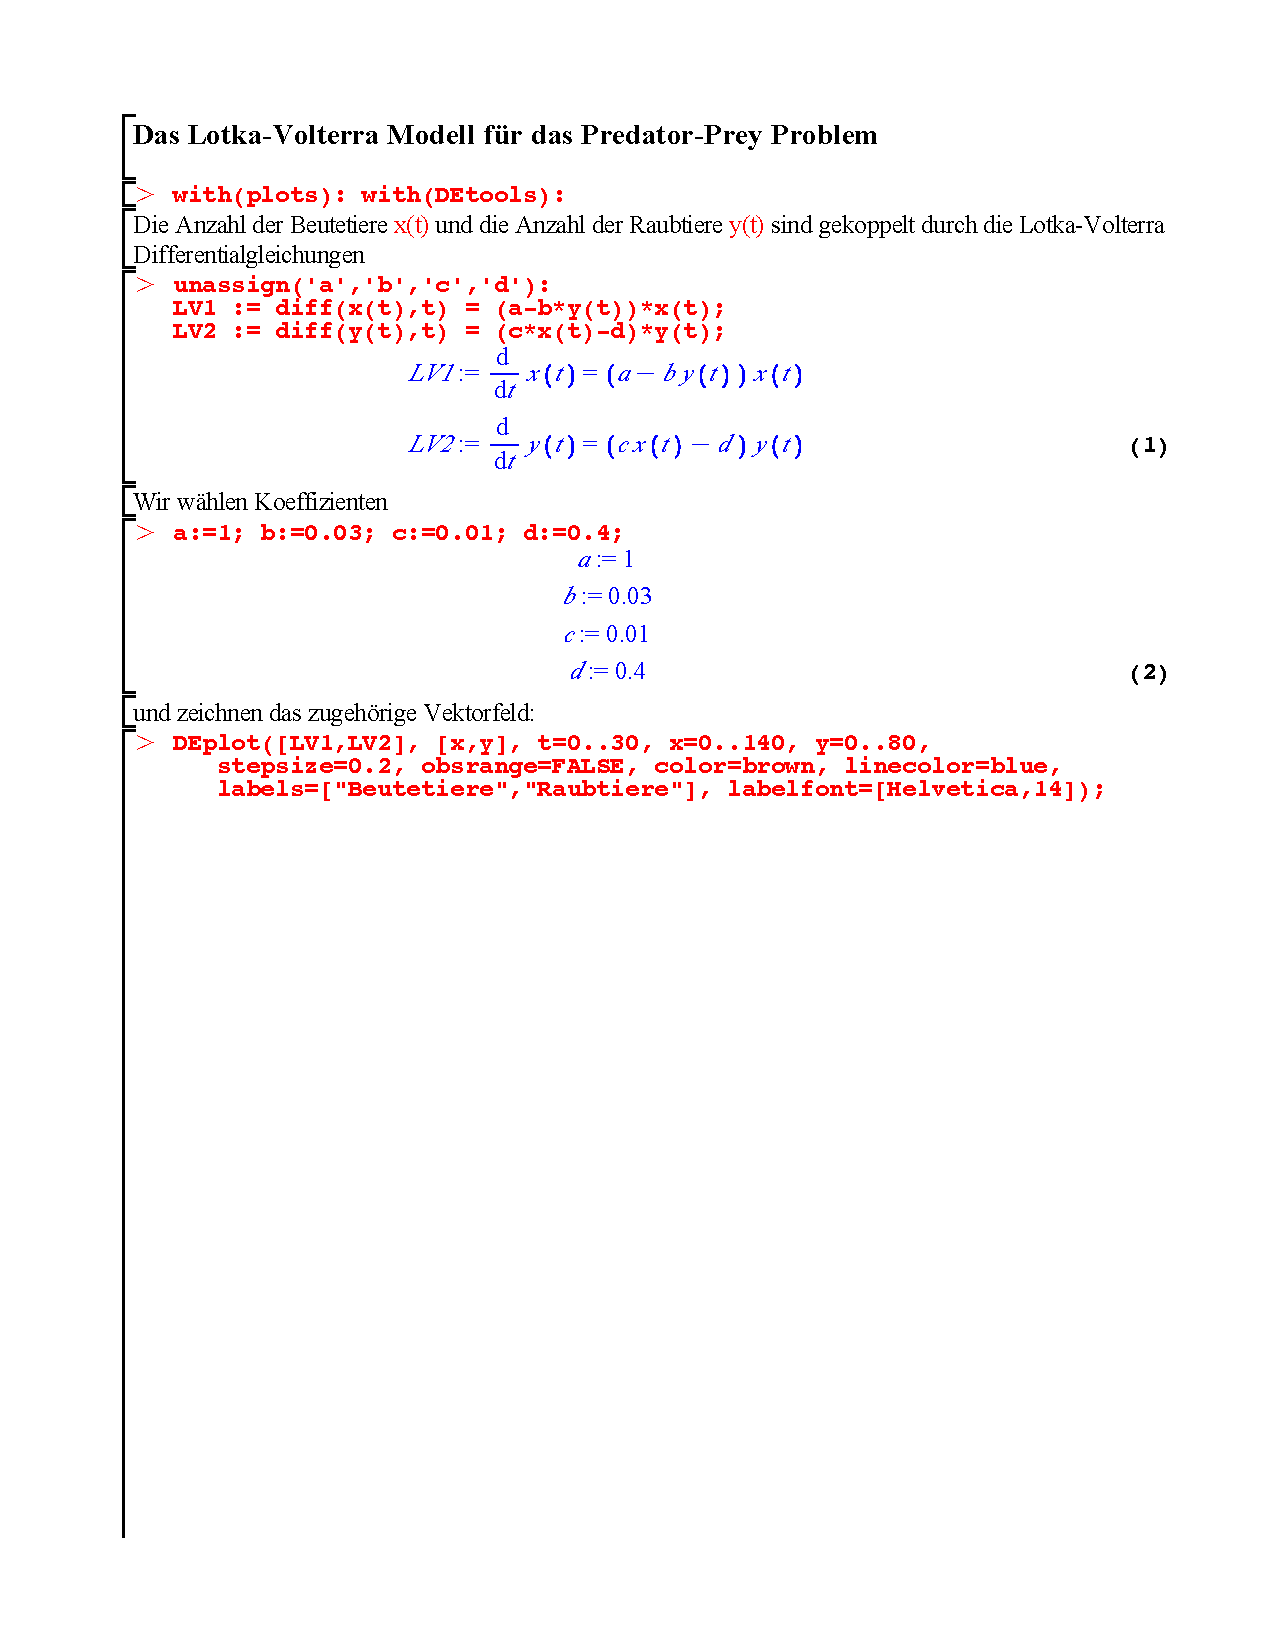
\includepdf[pages={1-7},addtotoc={1,section,1,Predator-Prey Modell,predatorprey}]{Predator-Prey}

\includepdf[pages={1},addtotoc={1,section,1,Lineare DifferentialGleichungen mit konstanten Koeffizienten,lindiffgleich}]{LinDiffGleich}
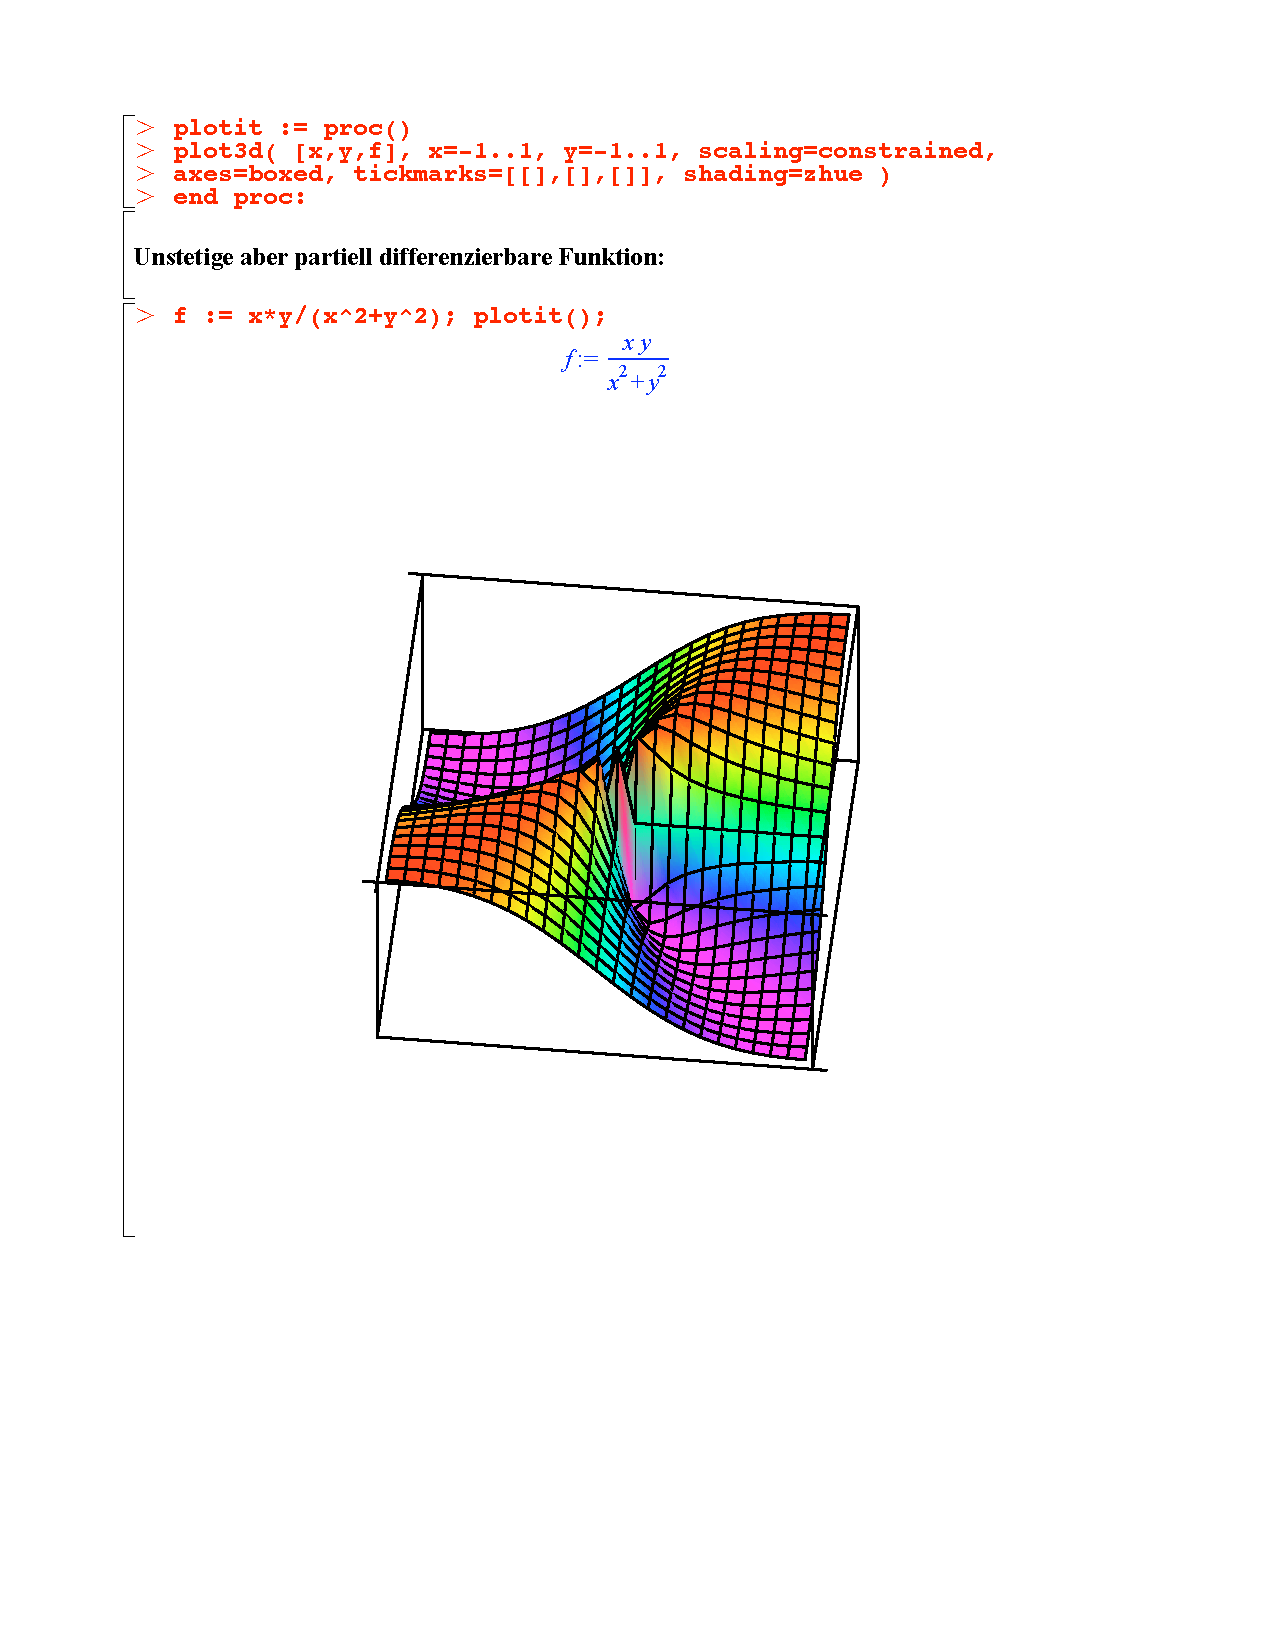
\includepdf[pages={1-5},addtotoc={1,section,1,Beispiele zum Thema Differenzierbarkeit,diffbarkeit}]{Diffbarkeit}
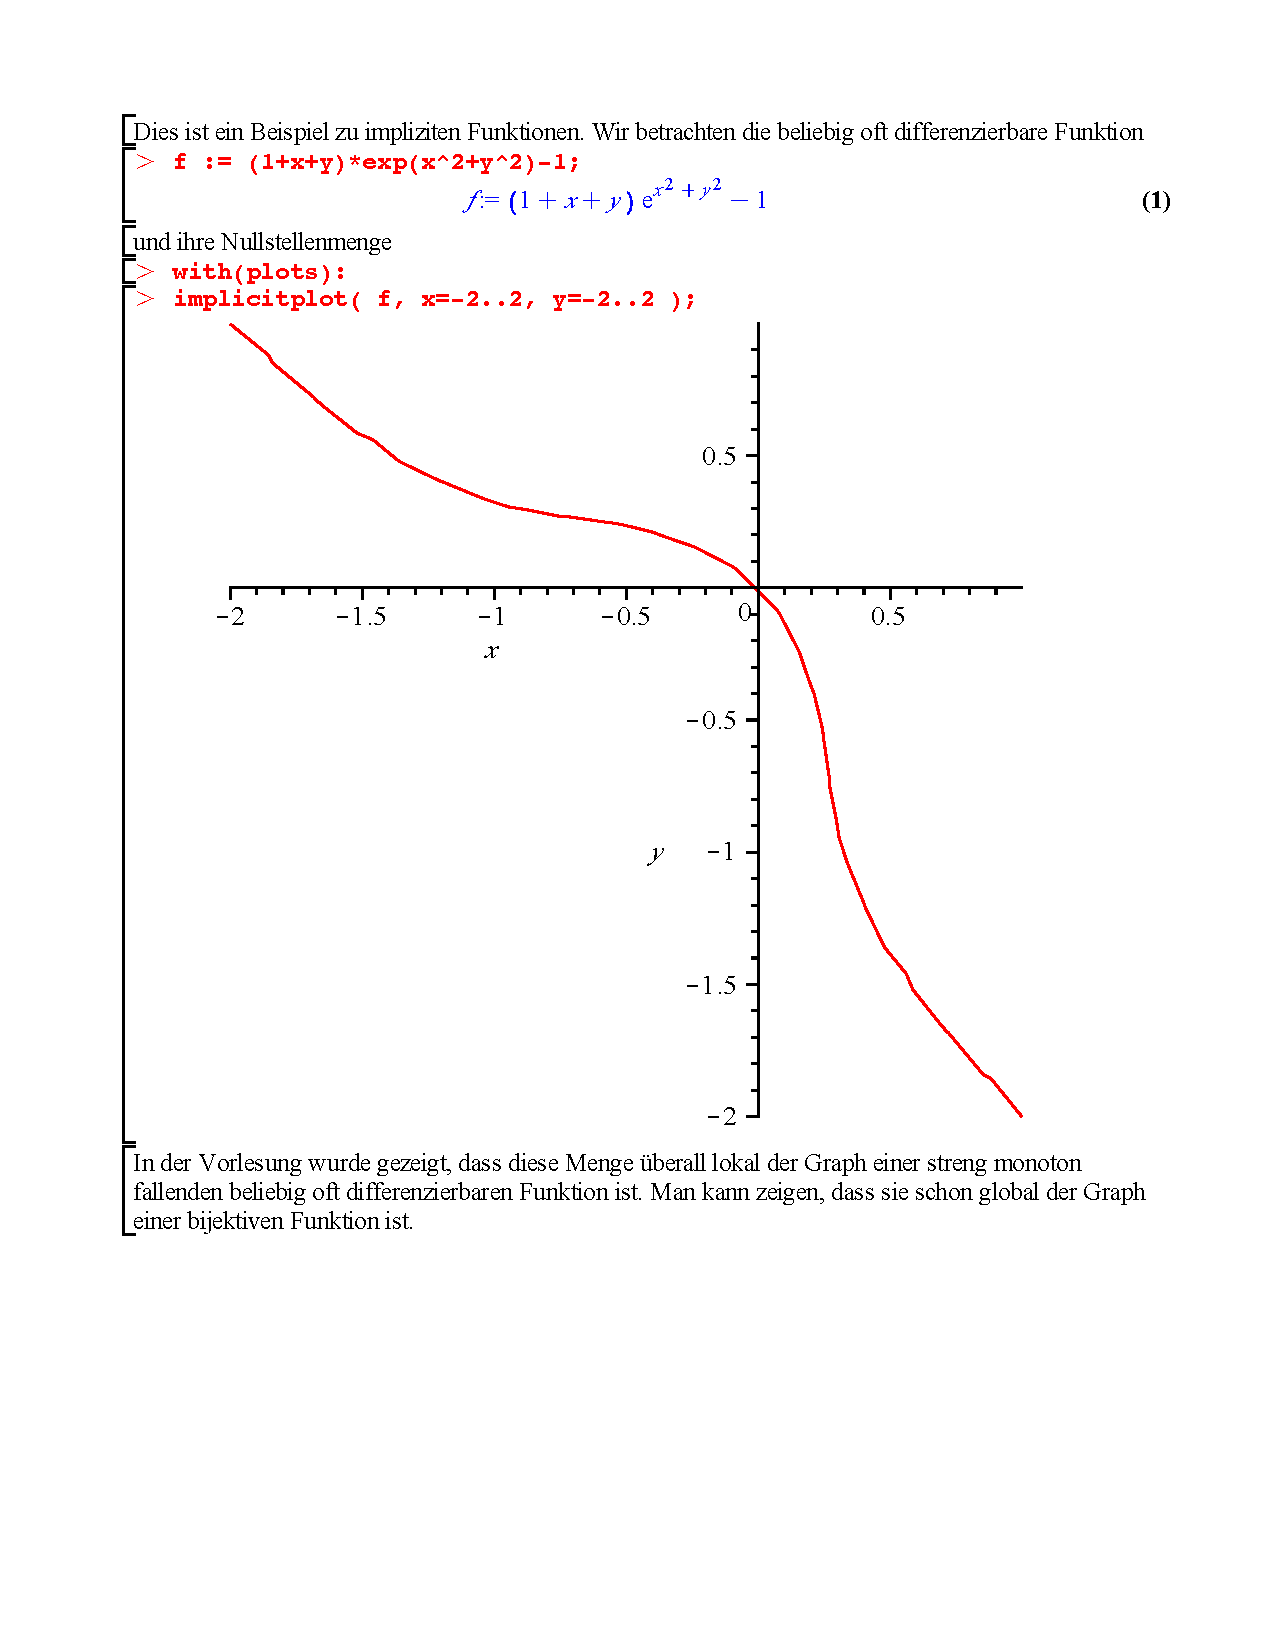
\includepdf[pages={1-3},addtotoc={1,section,1,Beispiele zum Thema Implizite Funktionen,implizitefunktion}]{ImpliziteFunktion}

\end{document}